\documentclass[a4paper,12pt]{article}

\usepackage{../xelatexhanaminvertical}
\usepackage{shijitsugan}
\usepackage{metalogo}

\title{資治通鑑 卷八十二 晉紀四\vspace{-3cm}}
%\author{司馬光}
\date{}

\begin{document}
\maketitle

\section*{はじめに}

\begin{spacing}{1.4}

本文書は、\yokorm{\XeLaTeX}で花園明朝フォントを使って縦書きをする方法を模索するためのサンプルとして作ったものです。

本文書の内容は、%
\href{http://dl.ndl.go.jp/}{国立国会図書館デジタルコレクション}%
で公開されている%
\href{http://dl.ndl.go.jp/info:ndljp/pid/1239900}{『続国訳漢文大成 經子史部第五卷』}%
\extrafootnote{%
\href{http://www.ndl.go.jp/jp/use/reproduction/index.html\#anchor02}{インターネット公開(保護期間満了)コンテンツ}%
です。}%
のうち、%
\href{http://dl.ndl.go.jp/info:ndljp/pid/1239900/156}{%
『資治通鑑』卷八十二(晉紀四)}%
のデータ起こしです。

ただし、改行などの体裁は変更しています。
また、テスト用に図(私が個人的に作成したもの)やリンクを挿入した箇所があります。
さらに、原注\footnote{原注はこの形式です。}とは区別した形式で、私的な備忘録\extrafootnote{私的な備忘録はこの形式です。}を注として追加しています。
注番号は元の番号と異なります。

お気づきの点やその他のコメントなどは、\yokorm{Twitter}で%
\href{https://twitter.com/pi\_\_yo\_\_ko}{\yokott{@pi\_\_yo\_\_ko}}%
までお気軽に御連絡ください。
\end{spacing}

\section*{ \ruby{世祖}{せい|そ}\ruby{武皇帝}{ぶ|くわう|てい}\ruby{下}{げ} }

\yearheading{二八九年・己酉}


%行末に%を書かないと組版したときに変なスペースが入ってしまうので、%を書いておく。

\ruby{太康}{たい|かう}%
\ruby{十年}{じふ|ねん}\footnote{西紀二八九年なり。}、%
\ruby{夏}{なつ}%
\ruby{四月}{し|ぐわつ}、%
\ruby{太廟}{たい|べう}%
\ruby{成}{な}る。%
\ruby{乙巳}{いつ|し}\extrafootnote{太康十年四月は、二八九年五月七日から二八九年六月五日まで。太康十年四月十一日・乙巳は、二八九年五月十七日。}、%
\ruby{祫祭}{かふ|さい}\footnote{大合祭なり。毀廟の主を、太祖に陳し、未だ廟を毀たざるの主をも、皆、升して太祖に合食する也。}す。%
\ruby{大赦}{たい|しや}す。%

\ruby{慕容廆}{ぼ|よう|くわい}、%
\ruby{使}{つかひ}を%
\ruby{遣}{つか}はし・%
\ruby{降}{くだ}らんと%
\ruby{請}{こ}ふ。%
\ruby{五月}{ご|ぐわつ}\extrafootnote{太康十年五月は、二八九年六月六日から七月四日まで。}、%
\ruby{詔}{みことのり}して、%
\ruby{廆}{くわい}を%
\ruby{鮮卑}{せん|ぴ}の%
\ruby{都督}{と|とく}に%
\ruby{拜}{はい}す。%
\ruby{廆}{くわい}、%
\ruby{何龕}{か|かん}に%
\ruby{謁見}{えつ|けん}す。%
\ruby{士大夫}{し|たい|ふ}の%
\ruby{禮}{れい}を%
\ruby{以}{もつ}て、%
\ruby{巾衣}{きん|い}\footnote{魏晉間、士大夫、尊貴に謁見するに、巾褠を著するを以て禮と爲す。褠は單衣なり。}して%
\ruby{門}{もん}に%
\ruby{到}{いた}る。%\ %禁則処理がうまくきいていないのでその対策に「\ 」を入れた。
\ruby{龕}{かん}、%
\ruby{兵}{へい}を%
\ruby{嚴}{げん}して%
\ruby{以}{もつ}て%
\ruby{之}{これ}を%
\ruby{見}{み}る。%
\ruby{廆}{くわい}%
\ruby{乃}{すなは}ち%
\ruby{改}{あらた}めて%
\ruby{戎衣}{じう|い}を%
\ruby{服}{ふく}して%
\ruby{入}{い}る。%
\ruby{人}{ひと}、%
\ruby{其}{そ}の%
\ruby{故}{ゆゑ}を%
\ruby{問}{と}ふ。%
\ruby{廆}{くわい}%
\ruby{曰}{い}はく、%
\begin{quoting}
『\ruby{主人}{しゆ|じん}、%
\ruby{禮}{れい}を%
\ruby{以}{もつ}て%
\ruby{客}{かく}を%
\ruby{待}{ま}たず。%
\ruby{客}{かく}、%
\ruby{何}{なに}をか%
\ruby{爲}{な}さんや』%
\end{quoting}
と。%
\ruby{龕}{かん}、%
\ruby{之}{これ}を%
\ruby{聞}{き}き、%
\ruby{甚}{はなは}だ%
\ruby{慙}{は}ぢ\footnote{胡三省曰はく、降を受くるは敵を受くるが如くし。邊に居るの帥、兵を嚴して以て四夷の客を見る、未だ過と爲さざるなり。何ぞ必ずしも以て慙と爲さんやと。}、%
\ruby{深}{ふか}く%
\ruby{之}{これ}を%
\ruby{敬異}{けい|い}す。%
\ruby{時}{とき}に%
\ruby{鮮卑}{せん|ぴ}の%
\ruby{宇文氏}{う|ぶん|し}・%\ %禁則処理がうまくきいていないのでその対策に「\ 」を入れた。%
\ruby{段氏}{だん|し}、%
\ruby{方}{まさ}に%
\ruby{彊}{つよ}く、%
\ruby{數〻}{しば|しば}%
\ruby{廆}{くわい}を%
\ruby{侵掠}{しん|りやく}す。%
\ruby{廆}{くわい}、%
\ruby{辭}{じ}を%
\ruby{卑}{ひく}くし%
\ruby{幣}{へい}を%
\ruby{厚}{あつ}くして%
\ruby{以}{もつ}て%
\ruby{之}{これ}に%
\ruby{事}{つか}ふ。%
\ruby{段國}{だん|こく}%
\ruby{單于}{ぜん|う}%
\ruby{階}{かい}、%
\ruby{女}{ぢよ}を%
\ruby{以}{もつ}て%
\ruby{廆}{くわい}に%
\ruby{妻}{めあは}す\footnote{慕容氏・段氏、遂に婚姻の國と爲る。}。%
\ruby{皝}{くわう}・%
\ruby{仁}{じん}・%
\ruby{昭}{せう}を%
\ruby{生}{う}む。%
\ruby{廆}{くわい}、%
\ruby{遼東}{れう|とう}の%
\ruby{僻遠}{へき|ゑん}なるを%
\ruby{以}{もつ}て、%
\ruby{徙}{うつ}りて%
\hypertarget{tokanoseizan}{%
\ruby{徒河}{と|か}\footnote{縣の名。故城は今の奉天省遼瀋道錦縣の西北にあり、靑山はその地の山の名なり。}の%
\ruby{靑山}{せい|ざん}に%
\ruby{居}{を}る}。%

%
\ruby{冬}{ふゆ}%
\ruby{十月}{じふ|ぐわつ}\extrafootnote{太康十年十月は、二八九年十月三十一日から二八九年十一月二十九日まで。}、%
\ruby{明堂}{めい|だう}%
\ruby{及}{およ}び%
\ruby{南郊}{なん|かう}の%
\ruby{五帝}{ご|てい}の%
\ruby{位}{くらゐ}を%
\ruby{復}{ふく}す\footnote{明堂・南郊より五帝の座を除くこと、\href{http://dl.ndl.go.jp/info:ndljp/pid/1239900/101}{七十九卷泰始二年}に見ゆ。}。%

%
\ruby{十一月}{じふ|いち|ぐわつ}%
\ruby{丙辰}{へい|しん}\extrafootnote{太康十年十一月に丙辰が見当たらないような……。ちなみに太康十年十月二十五日・丙辰なら二八九年十一月二十四日。}、%
\ruby{尚書令}{しやう|しよ|れい}%
\ruby{濟北}{せい|ほく}の%
\ruby{成侯}{せい|こう}%
\ruby{荀勗}{じゆん|きよく}・%
\ruby{卒}{しゆつ}す。%
\ruby{勗}{きよく}、%
\ruby{才思}{さい|し}%
\ruby{有}{あ}り、%
\ruby{善}{よ}く%
\ruby{人主}{じん|しゆ}の%
\ruby{意}{い}を%
\ruby{伺}{うかが}ふ。%
\ruby{是}{これ}を%
\ruby{以}{もつ}て%
\ruby{能}{よ}く%
\ruby{其}{そ}の%
\ruby{寵}{ちよう}を%
\ruby{固}{かた}くす。%
\ruby{久}{ひさ}しく%
\ruby{中書}{ちう|しよ}に%
\ruby{在}{あ}り、%
\ruby{專}{もつぱ}ら%
\ruby{機事}{き|じ}を%
\ruby{管}{つかさど}る。%
\ruby{尚書}{しやう|しよ}に%
\ruby{遷}{うつ}るに%
\ruby{及}{およ}びて、%
\ruby{甚}{はなは}だ%
\ruby{罔悵}{まう|ちやう}\footnote{志を失ひ恨望する貌。}たり。%
\ruby{人}{ひと}、%
\ruby{之}{これ}を%
\ruby{賀}{が}する%
\ruby{者}{もの}%
\ruby{有}{あ}り。%
\ruby{勗}{きよく}%
\ruby{曰}{い}はく、%
\begin{quoting}
『\ruby{我}{わ}が%
\ruby{鳳皇池}{ほう|わう|ち}を%
\ruby{奪}{うば}ふ。%
\ruby{諸君}{しよ|くん}%
\ruby{何}{なん}ぞ%
\ruby{賀}{が}するや』
\end{quoting}
と。%

\begin{figure}[htbp]
\centering
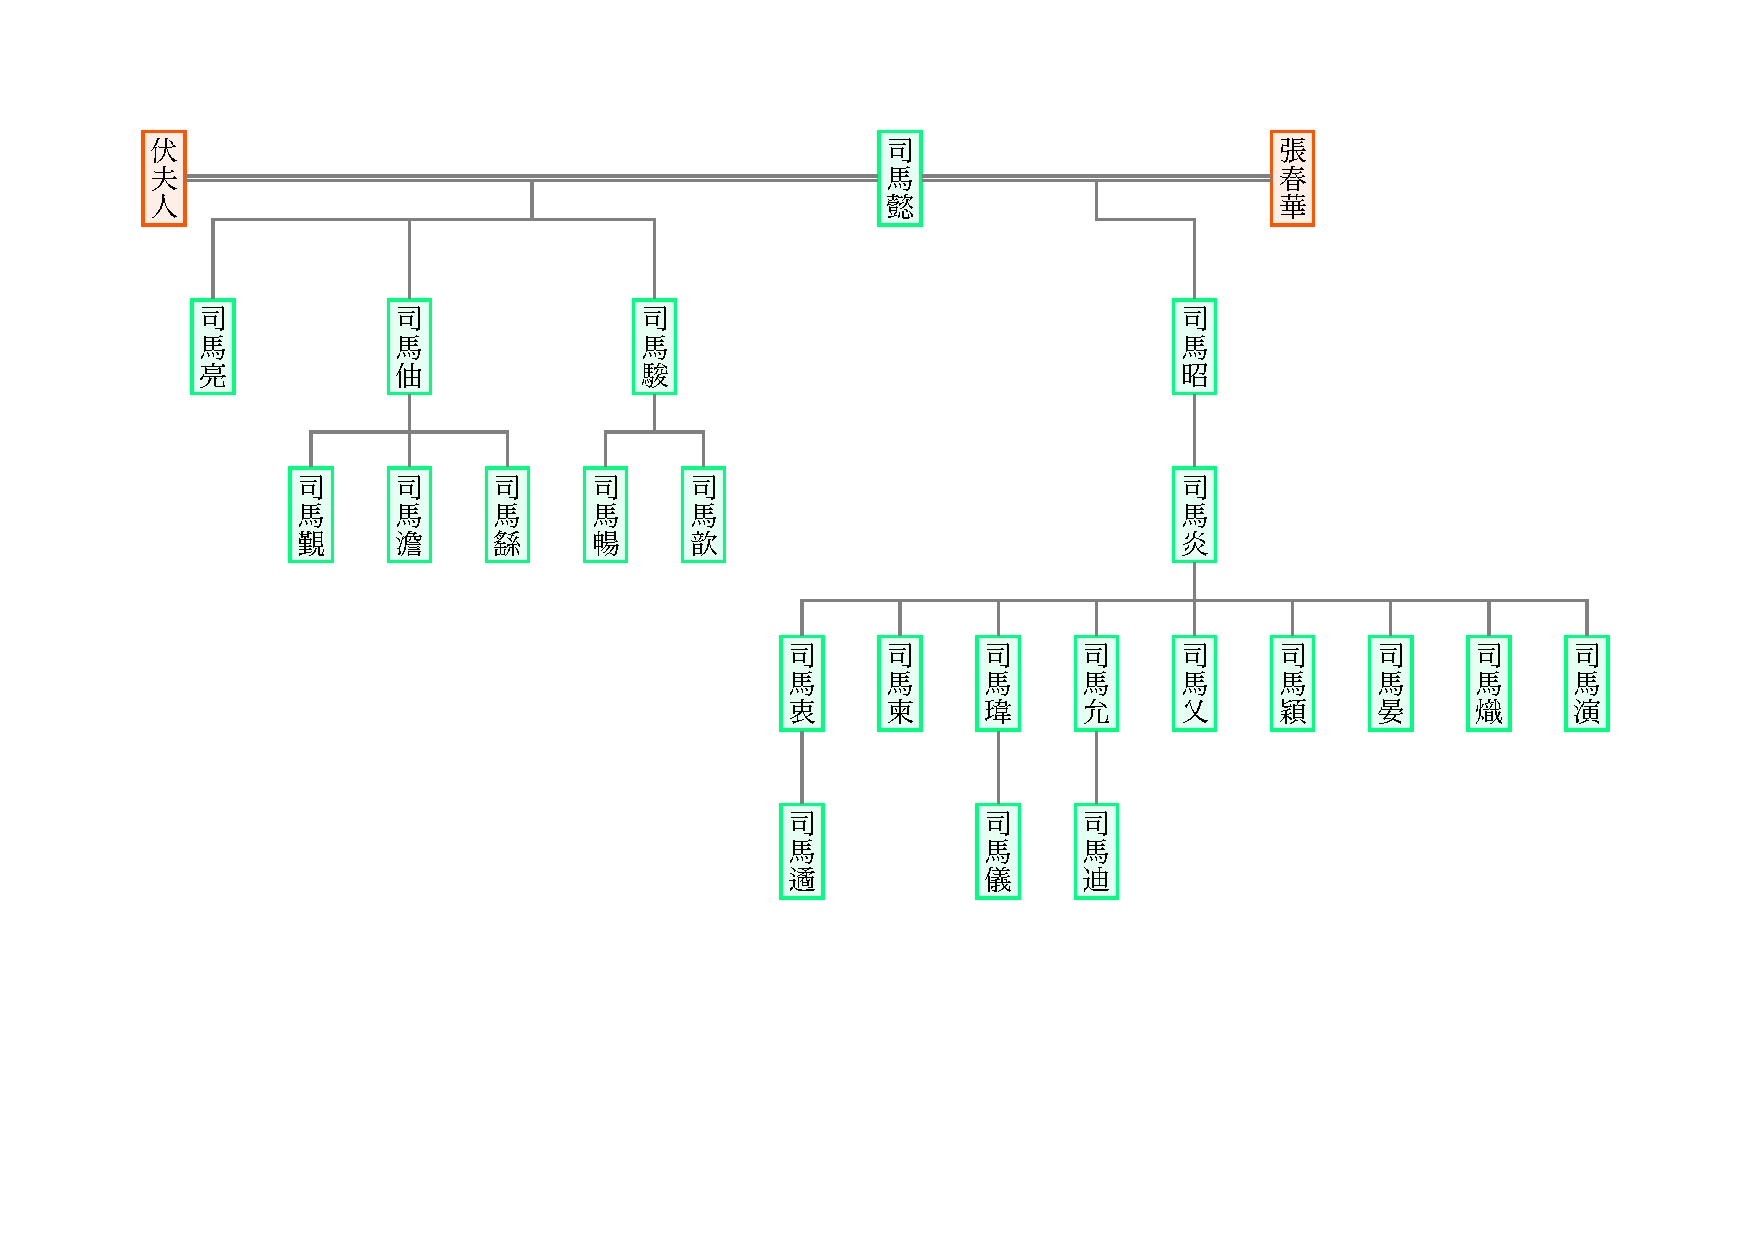
\includegraphics[width=13cm,angle=90]{ce_289-12-22.pdf}
\end{figure}

%
\ruby{帝}{てい}、%
\ruby{意}{い}を%
\ruby{聲色}{せい|しよく}に%
\ruby{極}{きは}め、%
\ruby{遂}{つひ}に・%
\ruby{疾}{やまひ}を%
\ruby{成}{な}すに%
\ruby{至}{いた}る。%
\ruby{楊駿}{やう|しゆん}、%
\ruby{汝南王}{じよ|なん|わう}%
\ruby{亮}{りやう}を%
\ruby{忌}{い}み、%
\ruby{之}{これ}を%
\ruby{排出}{はい|すゐ}す。%
\ruby{甲申}{かふ|しん}\extrafootnote{太康十年十一月二十三日・甲申は、二八九年十二月二十二日。}、%
\ruby{亮}{りやう}を%
\ruby{以}{もつ}て%
\ruby{侍中}{じ|ちう}・%
\ruby{大司馬}{たい|し|ば}・%
\ruby{假黃鉞}{か|くわう|ゑつ}%
\ruby{大都督}{たい|と|とく}と%
\ruby{爲}{な}し、%
\ruby{豫州}{よ|しう}の%
\ruby{諸軍事}{しよ|ぐん|じ}を%
\ruby{督}{とく}し、%
\ruby{許昌}{きよ|しやう}に%
\ruby{治}{ち}せしめ、%
\ruby{南陽王}{なん|やう|わう}%
\ruby{柬}{かん}を%
\ruby{徙}{うつ}して%
\ruby{秦王}{しん|わう}と%
\ruby{爲}{な}し、%
\ruby{關中}{くわん|ちう}の%
\ruby{諸軍事}{しよ|ぐん|じ}を%
\ruby{都督}{と|とく}せしめ、%
\ruby{始平王}{し|へい|わう}%
\ruby{瑋}{ゐ}を%
\ruby{楚王}{そ|わう}と%
\ruby{爲}{な}し、%
\ruby{荆州}{けい|しう}の%
\ruby{諸軍事}{しよ|ぐん|じ}を%
\ruby{都督}{と|とく}せしめ、%
\ruby{濮陽王}{ぼく|やう|わう}%
\ruby{允}{いん}を%
\ruby{淮南王}{わい|なん|わう}と%
\ruby{爲}{な}し、%
\ruby{揚江}{やう|かう}%
\ruby{二州}{に|しう}\footnote{\hyperlink{koushuu}{惠帝元康元年、揚州の豫章・鄱陽・廬陵・臨川・南康・建安・晉安、荊州の桂陽・安成・武昌、合はせて十郡を割きて江州を置く。}此の時未だ江州有らず、疑ふらくは江二の二字は衍ならんか。}の%
\ruby{諸軍事}{しよ|ぐん|じ}を%
\ruby{都督}{と|とく}せしめ、%
\ruby{竝}{ならび}に%
\ruby{節}{せつ}を%
\ruby{假}{か}して\footnote{晉の制、都督諸軍事に使持節あり、持節あり、假節あり。使持節は二千石以下を殺すを得。持節は官位無き人を殺す、若し軍事には使持節と同じ。假節は惟だ軍事のみに軍令を犯す者を殺すを得。}%
\ruby{國}{くに}に%
\ruby{之}{ゆ}かしむ。%
\ruby{皇子}{くわう|し}%
\ruby{乂}{かい}を%
\ruby{立}{た}てて%
\ruby{長沙王}{ちやう|さ|わう}と%
\ruby{爲}{な}し、%
\ruby{頴}{えい}を%
\ruby{成都王}{せい|と|わう}と%
\ruby{爲}{な}し、%
\ruby{晏}{あん}を%
\ruby{吳王}{ご|わう}と%
\ruby{爲}{な}し、%
\ruby{熾}{し}を%
\ruby{豫章王}{よ|しやう|わう}と%
\ruby{爲}{な}し、%
\ruby{演}{えん}を%
\ruby{代王}{だい|わう}と%
\ruby{爲}{な}し、%
\hypertarget{kouryouou}{%
\ruby{皇孫}{くわう|そん}%
\ruby{遹}{いつ}を%
\ruby{廣陵王}{くわう|りよう|わう}と%
\ruby{爲}{な}す。}%
\ruby{又}{また}、%
\ruby{淮南王}{わい|なん|わう}の%
\ruby{子}{こ}%
\ruby{迪}{てき}を%
\ruby{封}{ほう}じて%
\ruby{漢王}{かん|わう}と%
\ruby{爲}{な}し、%
\ruby{楚王}{そ|わう}の%
\ruby{子}{こ}%
\ruby{儀}{ぎ}を%
\ruby{毗陵王}{ひ|りよう|わう}と%
\ruby{爲}{な}し、%
\ruby{扶風王}{ふ|ふう|わう}%
\ruby{暢}{ちやう}を%
\ruby{徙}{うつ}して%
\ruby{順陽王}{じゆん|やう|わう}と%
\ruby{爲}{な}し、%
\ruby{暢}{ちやう}の%
\ruby{弟}{おとうと}%
\ruby{歆}{きん}を%
\ruby{新野公}{しん|や|こう}\footnote{晉の制、宗室の、郡公に封ぜらるる者は、制度、小國の王の如し。}と%
\ruby{爲}{な}す。%
\ruby{暢}{ちやう}は%
\ruby{駿}{しゆん}の%
\ruby{子}{こ}なり。%
\ruby{琅邪王}{らう|や|わう}%
\ruby{覲}{きん}の%
\ruby{弟}{おとうと}%
\ruby{澹}{たん}を%
\ruby{東武公}{とう|ぶ|こう}と%
\ruby{爲}{な}し、%
\ruby{繇}{えう}を%
\ruby{東安公}{とう|あん|こう}と%
\ruby{爲}{な}す。%
\ruby{覲}{きん}は%
\ruby{伷}{ちう}の%
\ruby{子}{こ}なり。%

%
\ruby{初}{はじ}め%
\ruby{帝}{てい}、%
\ruby{才人}{さい|じん}\footnote{女官の位、美人に次ぐ。晉の武帝、漢魏の制を采り、三夫人・九嬪の下に、美人・才人・中才人あり、爵、千石以下に\ruby{視}{なぞら}
ふ。}%
\ruby{謝玖}{しや|きう}を%
\ruby{以}{もつ}て%
\ruby{太子}{たい|し}に%
\ruby{賜}{たま}ふ。%
\ruby{皇孫}{くわう|そん}%
\ruby{遹}{いつ}を%
\ruby{生}{う}む。%
\ruby{宮中}{きう|ちう}、%
\ruby{嘗}{かつ}て%
\ruby{夜}{よる}、%
\ruby{火}{ひ}を%
\ruby{失}{しつ}す。%
\ruby{帝}{てい}、%
\ruby{樓}{ろう}に%
\ruby{登}{のぼ}りて%
\ruby{之}{これ}を%
\ruby{望}{のぞ}む。%
\ruby{遹}{いつ}、%
\ruby{年}{とし}%
\ruby{五歲}{ご|さい}。%
\ruby{帝}{てい}の%
\ruby{裾}{すそ}を%
\ruby{牽}{ひ}きて%
\ruby{闇中}{あん|ちう}に%
\ruby{入}{い}りて%
\ruby{曰}{い}はく、%
\begin{quoting}
『\ruby{暮夜}{ぼ|や}%
\ruby{倉猝}{さう|そつ}なり。%
\ruby{宜}{よろ}しく%
\ruby{非常}{ひ|じやう}に%
\ruby{備}{そな}ふべし。%
\ruby{人主}{じん|しゆ}を%
\ruby{照見}{せう|けん}せしむ%
\ruby{可}{べ}からず』
\end{quoting}
と。%
\ruby{帝}{てい}、%
\ruby{是}{これ}に%
\ruby{由}{よ}りて%
\ruby{之}{これ}を%
\ruby{奇}{き}とす。%
\ruby{嘗}{かつ}て%
\ruby{羣臣}{ぐん|しん}に%
\ruby{對}{たい}し、%
\begin{quoting}
『\ruby{遹}{いつ}、%
\ruby{宣帝}{せん|てい}に%
\ruby{似}{に}たり』
\end{quoting}
と%
\ruby{稱}{しよう}す。%
\ruby{故}{ゆゑ}に%
\ruby{天下}{てん|か}、%
\ruby{咸}{みな}、%
\ruby{之}{これ}に%
\ruby{歸仰}{き|ぎやう}す。%
\ruby{帝}{てい}、%
\ruby{太子}{たい|し}の%
\ruby{不才}{ふ|さい}なるを%
\ruby{知}{し}る。%
\ruby{然}{しか}れども%
\ruby{遹}{いつ}の%
\ruby{明慧}{めい|けい}なるを%
\ruby{恃}{たの}む。%
\ruby{故}{ゆゑ}に%
\ruby{廢立}{はい|りふ}の%
\ruby{心}{こころ}%
\ruby{無}{な}し。%
\ruby{復}{ま}た%
\ruby{王佑}{わう|いう}\footnote{王濟の弟なり。羊祜と竝に文帝に事ふ、帝これを寵任す。}の%
\ruby{謀}{はかりごと}を%
\ruby{用}{もち}ひ、%
\ruby{太子}{たい|し}の%
\ruby{母弟}{ぼ|てい}%
\ruby{柬}{かん}・%
\ruby{瑋}{ゐ}・%
\ruby{允}{いん}を%
\ruby{以}{もつ}て、%
\ruby{分}{わか}ちて%
\ruby{要害}{えう|がい}\footnote{雍・荆・揚の地をいふ。}を%
\ruby{鎭}{ちん}せしむ。%
\ruby{又}{また}、%
\ruby{楊氏}{やう|し}の%
\ruby{偪}{せま}らんことを%
\ruby{恐}{おそ}れ、%
\ruby{復}{ま}た%
\ruby{佑}{いう}を%
\ruby{以}{もつ}て%
\ruby{北軍中候}{ほく|ぐん|ちう|こう}と%
\ruby{爲}{な}し、%
\ruby{禁兵}{きん|ぺい}を%
\ruby{典}{つかさど}らしむ。%
\ruby{帝}{てい}、%
\ruby{皇孫}{くわう|そん}%
\ruby{遹}{いつ}の%
\ruby{爲}{た}めに、%
\ruby{高}{たか}く%
\ruby{僚佐}{れう|さ}を%
\ruby{選}{えら}び、%
\ruby{散騎常侍}{さん|き|じやう|じ}%
\ruby{劉寔}{りう|しよく}が%
\ruby{志行}{し|かう}%
\ruby{淸素}{せい|そ}なるを%
\ruby{以}{もつ}て、%
\ruby{命}{めい}じて%
\ruby{高陵王}{かう|りよう|わう}\extrafootnote{\hyperlink{kouryouou}{直前の段落には「\ruby{皇孫}{くわう|そん}\ruby{遹}{いつ}を\ruby{廣陵王}{くわう|りよう|わう}と\ruby{爲}{な}す。」とある}ので、どちらかが誤記なのではないか。}の
\ruby{傅}{ふ}と%
\ruby{爲}{な}す。%

%
\ruby{寔}{しよく}、%
\ruby{時俗}{じ|ぞく}・%
\ruby{進趣}{しん|しゆ}を%
\ruby{喜}{この}み%
\ruby{廉讓}{れん|じやう}%
\ruby{少}{すくな}きを%
\ruby{以}{もつ}て、%
\warichu{嘗テ崇讓論ヲ著シ}%
\ruby{初}{はじ}めて%
\ruby{官}{くわん}に%
\ruby{除}{ぢよ}せられ%
\ruby{謝章}{しや|しやう}を%
\ruby{通}{つう}ずる%
\ruby{者}{もの}をして・%
\ruby{必}{かなら}ず%
\ruby{賢}{けん}を%
\ruby{推}{お}し%
\ruby{能}{のう}に%
\ruby{讓}{ゆづ}りて・%
\ruby{乃}{すなは}ち%
\ruby{之}{これ}を%
\ruby{通}{つう}ずるを%
\ruby{得}{え}しめ・%
\ruby{一官}{いつ|くわん}%
\ruby{缺}{か}くるときは%
\ruby{則}{すなは}ち%
\ruby{人}{ひと}の%
\ruby{讓}{ゆづ}る%
\ruby{所}{ところ}と%
\ruby{爲}{な}ること%
\ruby{最}{もつと}も%
\ruby{多}{おほ}き%
\ruby{者}{もの}を%
\ruby{擇}{えら}びて%
\ruby{之}{これ}を%
\ruby{用}{もち}ひんことを%
\ruby{欲}{ほつ}し、%
\ruby[g]{以爲}{い}はく、%
\begin{quoting}
『\ruby{人情}{にん|じやう}、%
\ruby{爭}{あらそ}ふときは%
\ruby{則}{すなは}ち%
\ruby{己}{おのれ}の%
\ruby{如}{し}かざる%
\ruby{所}{ところ}を%
\ruby{毀}{そし}らんと%
\ruby{欲}{ほつ}し、%
\ruby{讓}{ゆづ}るときは%
\ruby{則}{すなは}ち%
\ruby{競}{きそ}うて%
\ruby{己}{おのれ}に%
\ruby{勝}{まさ}れるを%
\ruby{推}{お}す。%
\ruby{故}{ゆゑ}に%
\ruby{世}{よ}%
\ruby{爭}{あらそ}ふときは%
\ruby{則}{すなは}ち%
\ruby{優劣}{いう|れつ}%
\ruby{分}{わか}ち%
\ruby{難}{がた}く、%
\ruby{時}{とき}%
\ruby{讓}{ゆづ}るときは%
\ruby{則}{すなは}ち%
\ruby{賢智}{けん|ち}%
\ruby{顯}{あらは}れ%
\ruby{出}{い}づ。%
\ruby{此}{こ}の%
\ruby{時}{とき}に%
\ruby{當}{あた}りてや、%
\ruby{能}{よ}く%
\ruby{身}{み}を%
\ruby{退}{しりぞ}け%
\ruby{己}{おのれ}を%
\ruby{脩}{をさ}むるときは、%
\ruby{則}{すなは}ち%
\ruby{之}{これ}に%
\ruby{讓}{ゆづ}る%
\ruby{者}{もの}%
\ruby{多}{おほ}し。%
\ruby{貧賤}{ひん|せん}を%
\ruby{守}{まも}らんと%
\ruby{欲}{ほつ}すと%
\ruby{雖}{いへど}も、%
\ruby{得}{う}%
\ruby{可}{べ}からざるなり。%
\ruby{馳騖進趨}{ち|ぶ|しん|すう}して、%
\ruby{而}{しか}も%
\ruby{人}{ひと}に%
\ruby{讓}{ゆづ}られんことを%
\ruby{欲}{ほつ}するは、%
\ruby{猶}{な}ほ%
\ruby{却行}{きやく|かう}して%
\ruby{而}{しか}も%
\ruby{前}{すす}まんことを%
\ruby{求}{もと}むるがごときなり』
\end{quoting}
と。%

%
\ruby{淮南}{わい|なん}の%
\ruby{相}{しやう}%
\ruby{劉頌}{りう|しよう}・%
\ruby{上疏}{じやう|そ}して%
\ruby{曰}{い}はく、%
\begin{quoting}
『\ruby{陛下}{へい|か}、%
\ruby{以}{おも}へらく、%
\ruby{法禁}{はふ|きん}%
\ruby{寬縱}{くわん|じう}なること、%
\ruby{之}{これ}を%
\ruby{積}{つ}むこと%
\ruby{素}{そ}%
\ruby{有}{あ}り、%
\ruby{未}{いま}だ%
\ruby{一旦}{いつ|たん}に%
\ruby{直繩}{ちよく|じよう}を%
\ruby{以}{もつ}て%
\ruby{下}{しも}を%
\ruby{御}{ぎよ}す%
\ruby{可}{べ}からずと。%
\ruby{此}{こ}れ%
\ruby{誠}{まこと}に%
\ruby{時}{とき}の%
\ruby{宜}{よろ}しきなり。%
\ruby{然}{しか}れども%
\ruby{世}{よ}を%
\ruby{矯}{た}め%
\ruby{弊}{へい}を%
\ruby{救}{すく}ふに%
\ruby{至}{いた}りては、%
\ruby{自}{おのづか}ら%
\ruby{宜}{よろ}しく%
\ruby{漸}{やうや}く%
\ruby{淸肅}{せい|しゆく}に%
\ruby{就}{つ}くべし。%
\ruby{譬}{たと}へば%
\ruby{猶}{な}ほ%
\ruby{舟}{ふね}を%
\ruby{行}{や}るがごとし。%
\ruby{迅流}{じん|りう}を%
\ruby{橫截}{わう|せつ}せずと%
\ruby{雖}{いへど}も、%
\ruby{然}{しか}れども%
\ruby{當}{まさ}に%
\ruby{漸靡}{ぜん|び}\footnote{次第になびき從ふこと。水の勢に因りて漸靡して舟を行るをいふ。}して%
\ruby{往}{ゆ}き、%
\ruby{稍}{やうや}く%
\ruby{趨}{おもむ}く%
\ruby{所}{ところ}に%
\ruby{向}{むか}ふべし。%
\ruby{然}{しか}る%
\ruby{後}{のち}%
\ruby{濟}{わた}るを%
\ruby{得}{う}るなり。%
\ruby{泰始}{たい|し}より%
\ruby{以來}{い|らい}、%
\ruby{將}{まさ}に%
\ruby{三十年}{さん|じふ|ねん}ならんとす\footnote{帝、禪を受けて泰始と改元せしより、是に至るまで、二十五年。}。%
\ruby{凡}{およ}そ%
\ruby{諸}{もろもろ}の%
\ruby{事業}{じ|げふ}、%
\ruby{旣往}{き|わう}よりも%
\ruby{茂}{さかん}ならず。%
\ruby{陛下}{へい|か}の%
\ruby{明聖}{めい|せい}を%
\ruby{以}{もつ}て、%
\ruby{猶}{な}ほ%
\ruby{未}{いま}だ%
\ruby{叔世}{しゆく|せい}\footnote{末世なり。}の%
\ruby{敝}{へい}に%
\ruby{反}{はん}して、%
\ruby{以}{もつ}て%
\ruby{始初}{し|しよ}の%
\ruby{隆}{りう}を%
\ruby{成}{な}し、%
\ruby{之}{これ}を%
\ruby{後世}{こう|せい}に%
\ruby{傳}{つた}へず。%
\ruby{慮}{おもんぱかり}%
\ruby{無}{な}からざらんや。%
\ruby{夫}{か}の%
\ruby{異時}{い|じ}をして、%
\ruby{大業}{たい|げふ}%
\ruby{或}{あるひ}は%
\ruby{安}{やす}んぜざる%
\ruby{有}{あ}らしめば、%
\ruby{其}{そ}の%
\ruby{憂責}{いう|せき}、%
\ruby{猶}{な}ほ%
\ruby{陛下}{へい|か}に%
\ruby{在}{あ}らん。%
\ruby{臣}{しん}%
\ruby{聞}{き}く、%
\ruby{社稷}{しや|しよく}の%
\ruby{計}{けい}を%
\ruby{爲}{な}すは、%
\ruby{親賢}{しん|けん}を%
\ruby{封建}{ほう|けん}するに%
\ruby{若}{し}くは%
\ruby{莫}{な}しと。%
\ruby{然}{しか}れども%
\ruby{宜}{よろ}しく%
\ruby{審}{つまびら}かに%
\ruby{事埶}{じ|せい}を%
\ruby{量}{はか}るべし。%
\ruby{諸侯}{しよ|こう}の・%
\ruby{義}{ぎ}に%
\ruby{率}{したが}つて%
\ruby{動}{うご}く%
\ruby{者}{もの}をして、%
\ruby{其}{そ}の%
\ruby{力}{ちから}、%
\ruby{以}{もつ}て%
\ruby{京邑}{けい|いふ}を%
\ruby{維帶}{ゐ|たい}するに%
\ruby{足}{た}らしむ%
\ruby{可}{べ}し。%
\ruby{若}{も}し%
\ruby{禍心}{くわ|しん}を%
\ruby{包藏}{はう|ざう}せば、%
\ruby{其}{そ}の%
\ruby{埶}{いきほひ}、%
\ruby{獨}{ひと}り%
\ruby{以}{もつ}て%
\ruby{爲}{な}す%
\ruby{有}{あ}るに%
\ruby{足}{た}らざらしめよ。%
\ruby{其}{そ}の%
\ruby{此}{これ}を%
\ruby{齊}{ととの}ふること%
\ruby{甚}{はなは}だ%
\ruby{難}{かた}し。%
\ruby{陛下}{へい|か}、%
\ruby{宜}{よろ}しく%
\ruby{古今}{こ|こん}に%
\ruby{達}{たつ}するの%
\ruby{士}{し}と、%
\ruby{深}{ふか}く%
\ruby{共}{とも}に%
\ruby{之}{これ}を%
\ruby{籌}{はか}るべし。%
\ruby{周}{しう}の%
\ruby{諸侯}{しよ|こう}、%
\ruby{罪}{つみ}%
\ruby{有}{あ}れば、%
\ruby{其}{そ}の%
\ruby{身}{み}を%
\ruby{誅放}{ちう|はう}すれども、%
\ruby{而}{しか}も%
\ruby{國祚}{こく|そ}%
\ruby{泯}{ほろ}びず\footnote{周、\href{https://ja.wikipedia.org/wiki/\%E5\%93\%80\%E5\%85\%AC_(\%E6\%96\%89)}{齊の哀公}を烹て、而も\href{https://ja.wikipedia.org/wiki/\%E8\%83\%A1\%E5\%85\%AC_(\%E6\%96\%89)}{其の弟靜}を立て、\href{https://ja.wikipedia.org/wiki/\%E5\%AE\%A3\%E7\%8E\%8B_(\%E5\%91\%A8)}{宣王}、\href{https://ja.wikipedia.org/wiki/\%E5\%BB\%83\%E5\%85\%AC_(\%E9\%AD\%AF)}{魯侯伯御}を誅して而も\href{https://ja.wikipedia.org/wiki/\%E5\%AD\%9D\%E5\%85\%AC_(\%E9\%AD\%AF)}{孝公}を立つるの類の如し。}。%
\ruby{漢}{かん}の%
\ruby{諸侯}{しよ|こう}、%
\ruby{罪}{つみ}%
\ruby{有}{あ}り、%
\ruby{或}{あるひ}は%
\ruby{子}{こ}%
\ruby{無}{な}き%
\ruby{者}{もの}は、%
\ruby{國}{くに}%
\ruby{隨}{したが}つて%
\ruby{以}{もつ}て%
\ruby{亡}{ほろ}ぶ。%
\ruby{今}{いま}、%
\ruby{宜}{よろ}しく%
\ruby{漢}{かん}の%
\ruby{敝}{へい}に%
\ruby{反}{はん}し、%
\ruby{周}{しう}の%
\ruby{舊}{きう}に%
\ruby{循}{したが}ふべし。%
\ruby{則}{すなは}ち%
\ruby{下}{しも}%
\ruby{固}{かた}くして%
\ruby{上}{かみ}%
\ruby{安}{やす}からん。%
\ruby{天下}{てん|か}は%
\ruby{至大}{し|だい}、%
\ruby{萬事}{ばん|じ}は%
\ruby{至衆}{し|しう}。%
\ruby{人君}{じん|くん}は%
\ruby{至少}{し|せう}、%
\ruby{天日}{てん|じつ}に%
\ruby{同}{おな}じ。%
\ruby{是}{ここ}を%
\ruby{以}{もつ}て、%
\ruby{聖王}{せい|わう}の%
\ruby{化}{くわ}は、%
\ruby{要}{えう}を%
\ruby{己}{おのれ}に%
\ruby{執}{と}り、%
\ruby{務}{つとめ}を%
\ruby{下}{しも}に%
\ruby{委}{ゆだ}ぬ。%
\ruby{勞}{らう}を%
\ruby{惡}{にく}みて%
\ruby{逸}{いつ}を%
\ruby{好}{この}むに%
\ruby{非}{あら}ず。%
\ruby{誠}{まこと}に%
\ruby{政體}{せい|たい}%
\ruby{宜}{よろ}しく%
\ruby{然}{しか}るべきを%
\ruby{以}{もつ}てなり。%
\ruby{夫}{そ}れ%
\ruby{事}{こと}の%
\ruby{始}{はじめ}に%
\ruby{居}{を}りて%
\ruby{以}{もつ}て%
\ruby{能否}{のう|ひ}を%
\ruby{別}{わか}つは、%
\ruby{甚}{はなは}だ・%
\ruby{察}{さつ}し%
\ruby{難}{がた}きなり。%
\ruby{成敗}{せい|はい}に%
\ruby{因}{よ}りて%
\ruby{以}{もつ}て%
\ruby{功罪}{こう|ざい}を%
\ruby{分}{わか}つは、%
\ruby{甚}{はなは}だ・%
\ruby{識}{し}り%
\ruby{易}{やす}きなり。%
\ruby{今}{いま}、%
\ruby{陛下}{へい|か}、%
\ruby{每}{つね}に%
\ruby{始}{はじめ}を%
\ruby{造}{な}すに%
\ruby{精}{くは}しくして、%
\ruby{終}{をはり}を%
\ruby{考}{かう}するに%
\ruby{怠}{おこた}る。%
\ruby{此}{こ}れ%
\ruby{政功}{せい|こう}の%
\ruby{未}{いま}だ%
\ruby{善}{よ}からざる%
\ruby[g]{所以}{ゆゑん}なり。%
\ruby{人主}{じん|しゆ}、%
\ruby{誠}{まこと}に%
\ruby{能}{よ}く%
\ruby{易}{い}\footnote{簡易。}に%
\ruby{居}{を}り%
\ruby{要}{えう}を%
\ruby{執}{と}り、%
\ruby{功罪}{こう|ざい}を%
\ruby{成敗}{せい|はい}の%
\ruby{後}{のち}に%
\ruby{論}{ろん}ずれば、%
\ruby{則}{すなは}ち%
\ruby{羣下}{ぐん|か}、%
\ruby{其}{そ}の%
\ruby{誅賞}{ちう|しやう}を%
\ruby{逃}{のが}るる%
\ruby{所}{ところ}%
\ruby{無}{な}し。%
\ruby{古}{いにしへ}は%
\ruby{六卿}{りく|けい}\footnote{周禮に、天官冢宰・地官司徒・春官宗伯・夏官司馬・秋官司寇・冬官司空、是れを六卿と爲す、而して冢宰これを總ぶ。}、%
\ruby{職}{しよく}を%
\ruby{分}{わか}ち、%
\ruby{冢宰}{ちよう|さい}を%
\ruby{師}{し}と%
\ruby{爲}{な}す。%
\ruby{秦漢}{しん|かん}%
\ruby{已來}{い|らい}、%
\ruby{九列}{きう|れつ}、%
\ruby{事}{こと}を%
\ruby{執}{と}り、%
\ruby{丞相}{じよう|しやう}・%
\ruby{都總}{と|そう}す。%
\ruby{今}{いま}、%
\ruby{尚書}{しやう|しよ}・%
\ruby{制斷}{せい|だん}し、%
\ruby{諸卿}{しよ|けい}、%
\ruby{成}{せい}を%
\ruby{奉}{ほう}ず\footnote{漢の光武以來、吏事を以て尚書を責め、事、臺閣に歸し、諸卿は成を奉ずるのみ。}。%
\ruby{古制}{こ|せい}に%
\ruby{於}{おい}て、%
\ruby{太}{はなは}だ%
\ruby{重}{おも}しと%
\ruby{爲}{な}す。%
\ruby{衆事}{しう|じ}を%
\ruby{出}{いだ}して%
\ruby{外寺}{ぐわい|じ}\footnote{諸卿の官廳。寺は官廳をいふ。}に%
\ruby{付}{ふ}し・%
\ruby{之}{これ}を%
\ruby{專}{もつぱ}らにするを%
\ruby{得}{え}しめ・%
\ruby{尚書}{しやう|しよ}は%
\ruby{大綱}{たい|かう}を%
\ruby{統領}{とう|りやう}すること・%
\ruby{丞相}{じよう|しやう}の%
\ruby{爲}{しわざ}の%
\ruby{若}{ごと}くす%
\ruby{可}{べ}し。%
\ruby{歲終}{さい|しう}に、%
\ruby{功}{こう}を%
\ruby{課}{くわ}し%
\ruby{簿}{ぼ}を%
\ruby{校}{かう}し、%
\ruby{賞罰}{しやう|ばつ}せんのみ。%
\ruby{斯}{こ}れ%
\ruby{亦}{また}%
\ruby{可}{か}なり。%
\ruby{今}{いま}、%
\ruby{動}{うご}くに%
\ruby{皆}{みな}%
\ruby{成}{せい}を%
\ruby{上}{かみ}に%
\ruby{受}{う}く。%
\ruby{上}{かみ}の%
\ruby{失}{うしな}ふ%
\ruby{所}{ところ}、%
\ruby{復}{ま}た%
\ruby{以}{もつ}て%
\ruby{下}{しも}を%
\ruby{罪}{つみ}するを%
\ruby{得}{え}ず。%
\ruby{歲終}{さい|しう}に、%
\ruby{事功}{じ|こう}%
\ruby{建}{た}たざるも、%
\ruby{責}{せ}むる%
\ruby{所}{ところ}を%
\ruby{知}{し}らざるなり。%
\ruby{夫}{そ}れ%
\ruby{細過}{さい|くわ}%
\ruby{謬妄}{びう|ばう}は、%
\ruby{人情}{にん|じやう}の%
\ruby{必}{かなら}ず%
\ruby{有}{あ}る%
\ruby{所}{ところ}なり。%
\ruby{而}{しか}して%
\ruby{悉}{ことごと}く%
\ruby{糾}{ただ}すに%
\ruby{法}{はふ}を%
\ruby{以}{もつ}てせば、%
\ruby{則}{すなは}ち%
\ruby{朝野}{てう|や}、%
\ruby{立人}{りつ|じん}\footnote{晉書劉頌傳には全人に作る。}%
\ruby{無}{な}からん。%
\ruby{近世}{きん|せい}%
\ruby{以來}{い|らい}、%
\ruby{監司}{かん|し}\footnote{御史臺の官及び諸州の刺史は皆監司なり。}たる%
\ruby{者}{もの}、%
\ruby{類}{おほむ}ね%
\ruby{大綱}{たい|かう}をば%
\ruby{振}{ふる}はずして、%
\ruby{微過}{び|くわ}をば%
\ruby{必}{かなら}ず%
\ruby{擧}{あ}ぐ。%
\ruby{蓋}{けだ}し%
\ruby{豪彊}{がう|きやう}を%
\ruby{畏避}{ゐ|ひ}するに%
\ruby{由}{よ}る。%
\ruby{而}{しか}して%
\ruby{又}{また}、%
\ruby{職事}{しよく|じ}の%
\ruby{曠}{むな}しきを%
\ruby{懼}{おそ}れ、%
\ruby{則}{すなは}ち%
\ruby{密網}{みつ|まう}を%
\ruby{謹}{つつし}みて%
\ruby{以}{もつ}て%
\ruby{微罪}{び|ざい}を%
\ruby{羅}{ら}し、%
\ruby{奏劾}{そう|がい}をして%
\ruby{相}{あひ}%
\ruby{接}{せつ}せしむ。%
\ruby{狀}{じやう}、%
\ruby{公}{こう}を%
\ruby{盡}{つく}すに%
\ruby{似}{に}たれども、%
\ruby{法}{はふ}を%
\ruby{撓}{たわ}ますこと%
\ruby{其}{そ}の%
\ruby{中}{うち}に%
\ruby{在}{あ}り。%
\ruby{是}{ここ}を%
\ruby{以}{もつ}て、%
\ruby{聖王}{せい|わう}は、%
\ruby{碎密}{さい|みつ}\footnote{繁瑣微密。}の%
\ruby{案}{あん}を%
\ruby{善}{よ}しとせずして、%
\ruby{必}{かなら}ず%
\ruby{凶猾}{きよう|くわつ}の%
\ruby{奏}{そう}を%
\ruby{責}{せ}む。%
\ruby{則}{すなは}ち%
\ruby{政}{まつりごと}を%
\ruby{害}{がい}するの%
\ruby{姦}{かん}、%
\ruby{自然}{し|ぜん}に%
\ruby{禽}{とりこ}にせらる。%
\ruby{夫}{そ}れ%
\ruby{創業}{さう|げふ}の%
\ruby{勳}{くん}は、%
\ruby{教}{けう}を%
\ruby{立}{た}て%
\ruby{制}{せい}を%
\ruby{定}{さだ}むるに%
\ruby{在}{あ}り。%
\ruby{遺風}{ゐ|ふう}をして%
\ruby{人心}{じん|しん}を%
\ruby{繫}{つな}ぎ、%
\ruby{餘烈}{よ|れつ}をして%
\ruby{幼弱}{えう|じやく}を%
\ruby{匡}{ただ}さしむ。%
\ruby{後世}{こう|せい}、%
\ruby{之}{これ}に%
\ruby{憑}{よ}れば、%
\ruby{昏}{くら}しと%
\ruby{雖}{いへど}も%
\ruby{猶}{な}ほ%
\ruby{明}{あきら}かなるがごとく、%
\ruby{愚}{ぐ}なりと%
\ruby{雖}{いへど}も%
\ruby{智}{ち}なるが%
\ruby{若}{ごと}し\footnote{法制修まり明かなるときは、後嗣昏愚なりと雖も、據依する所あり、其治猶ほ明智の\ruby{爲}{しわざ}の若きを言ふ。}。%
\ruby{乃}{すなは}ち%
\ruby{尚}{たつと}ぶに%
\ruby{足}{た}るなり。%
\ruby{夫}{か}の・%
\ruby{官署}{くわん|しよ}を%
\ruby{脩飾}{しう|しよく}するに%
\ruby{至}{いた}るまで、%
\ruby{凡}{およ}そ%
\ruby{諸}{もろもろ}の%
\ruby{作役}{さく|えき}は、%
\ruby{恒}{つね}に・%
\ruby{太}{はなは}だ%
\ruby{過}{す}ぐるを%
\ruby{傷}{いた}む。%
\ruby{擧}{あが}らざるを%
\ruby{患}{うれ}へず。%
\ruby{此}{こ}れ%
\ruby{將來}{しやう|らい}、%
\ruby{陛下}{へい|か}を%
\ruby{須}{ま}たずして%
\ruby{自}{おのづか}ら%
\ruby{能}{よ}くする%
\ruby{所}{ところ}の%
\ruby{者}{もの}なり。%
\ruby{今}{いま}、%
\ruby{須}{ま}たざる%
\ruby{所}{ところ}を%
\ruby{勤}{つと}め、%
\ruby{以}{もつ}て%
\ruby{憑}{よ}る%
\ruby{所}{ところ}を%
\ruby{傷}{やぶ}るは、%
\ruby{竊}{ひそか}に%
\ruby{以}{もつ}て%
\ruby{過}{あやま}てりと%
\ruby{爲}{な}す』
\end{quoting}
と。%
\ruby{帝}{てい}、%
\ruby{皆}{みな}、%
\ruby{用}{もち}ふる%
\ruby{能}{あた}はず。%

%
\ruby{詔}{みことのり}して、%
\ruby{劉淵}{りう|えん}を%
\ruby{以}{もつ}て%
\ruby{匈奴}{きよう|ど}%
\ruby{北部}{ほく|ぶ}の%
\ruby{都尉}{と|ゐ}\footnote{時に匈奴五部の帥を改めて五部都尉と爲す。}と%
\ruby{爲}{な}す。%
\ruby{淵}{えん}、%
\ruby{財}{ざい}を%
\ruby{輕}{かろ}んじ%
\ruby{施}{し}を%
\ruby{好}{この}み、%
\ruby{心}{こころ}を%
\ruby{傾}{かたむ}け%
\ruby{物}{もの}に%
\ruby{接}{せつ}す。%
\ruby{五部}{ご|ぶ}の%
\ruby{豪桀}{がう|けつ}、%
\ruby{幽冀}{いう|き}の%
\ruby{名儒}{めい|じゆ}、%
\ruby{多}{おほ}く%
\ruby{往}{ゆ}きて%
\ruby{之}{これ}に%
\ruby{歸}{き}す。%

%
\ruby{奚軻}{けい|か}\footnote{夷種なり。}の%
\ruby{男女}{だん|ぢよ}%
\ruby{十萬口}{じふ|まん|こう}、%
\ruby{來}{きた}り%
\ruby{降}{くだ}る。%

\section*{\ruby{孝惠皇帝}{かう|けい|くわう|てい}\footnote{諱は衷、字は正度、武帝の第二子なり。}\ruby{上}{じやう}の\ruby{上}{じやう}}

\yearheading{二九〇年・庚戌}
%
\ruby{永熙}{えい|き}%
\ruby{元年}{ぐわん|ねん}\footnote{西紀二九〇年なり。ここに記するが如く、正月朔、武帝は太熙と改元せるを、三月、帝崩じて惠帝立つや、更に改元して永熙といへるなり。}%
\ruby{春}{はる}%
\ruby{正月}{しやう|ぐわつ}%
\ruby{辛酉}{しん|いう}%
\ruby{朔}{さく}\extrafootnote{太熙元年一月一日・辛酉は、二九〇年一月二十八日。}、%
\ruby{太熙}{たい|き}と%
\ruby{改元}{かい|げん}す。%

%
\ruby{己巳}{き|し}\extrafootnote{太熙元年一月九日・己巳は、二九〇年二月五日。}、%
\ruby{王渾}{わう|こん}を%
\ruby{以}{もつ}て%
\ruby{司徒}{し|と}と%
\ruby{爲}{な}す。%

%
\ruby{司空}{し|くう}%
\ruby{侍中}{じ|ちう}%
\ruby{尚書令}{しやう|しよ|れい}%
\ruby{衞瓘}{ゑい|くわん}の%
\ruby{子}{こ}%
\ruby{宣}{せん}、%
\ruby{繁昌公主}{はん|しやう|こう|しゆ}に%
\ruby{尚}{しやう}す。%
\ruby{宣}{せん}、%
\ruby{酒}{さけ}を%
\ruby{嗜}{たしな}み、%
\ruby{過失}{くわ|しつ}%
\ruby{多}{おほ}し。%
\ruby{楊駿}{やう|しゆん}、%
\ruby{瓘}{くわん}を%
\ruby{惡}{にく}み、%
\ruby{之}{これ}を%
\ruby{逐}{お}はんと%
\ruby{欲}{ほつ}す。%
\ruby{乃}{すなは}ち%
\ruby{黃門}{くわう|もん}と%
\ruby{謀}{はか}り、%
\ruby{共}{とも}に%
\ruby{宣}{せん}を%
\ruby{毀}{そし}り、%
\ruby{武帝}{ぶ|てい}に%
\ruby{勸}{すす}めて%
\ruby{公主}{こう|しゆ}を%
\ruby{奪}{うば}はしむ。%
\ruby{瓘}{くわん}%
\ruby{慚}{は}ぢ%
\ruby{懼}{おそ}れ、%
\ruby{老}{らう}を%
\ruby{告}{つ}げて%
\ruby{位}{くらゐ}を%
\ruby{遜}{のが}る。%
\ruby{詔}{みことのり}して、%
\ruby{瓘}{くわん}の%
\ruby{位}{くらゐ}を%
\ruby{太保}{たい|はう}に%
\ruby{進}{すす}め、%
\ruby{公}{こう}\footnote{瓘は、菑陽公に封ぜらる。}を%
\ruby{以}{もつ}て%
\ruby{第}{てい}に%
\ruby{就}{つ}かしむ。%

%
\ruby{劇陽}{げき|やう}の%
\ruby{康子}{かう|し}%
\ruby{魏舒}{ぎ|じよ}・%
\ruby{薨}{こう}ず。%

%
\ruby{三月}{さん|ぐわつ}%
\ruby{甲子}{かふ|し}\extrafootnote{太熙元年三月五日・甲子は、二九〇年四月一日。}、%
\ruby{右光祿大夫}{いう|くわう|ろく|たい|ふ}%
\ruby{石鑒}{せき|かん}を%
\ruby{以}{もつ}て%
\ruby{司空}{し|くう}と%
\ruby{爲}{な}す。%

%
\ruby{帝}{てい}、%
\ruby{疾}{やまひ}%
\ruby{篤}{あつ}し。%
\ruby{未}{いま}だ%
\ruby{顧命}{こ|めい}%
\ruby{有}{あ}らず。%
\ruby{勳舊}{くん|きう}の%
\ruby{臣}{しん}、%
\ruby{多}{おほ}く%
\ruby{已}{すで}に%
\ruby{物故}{ぶつ|こ}す。%
\ruby{侍中}{じ|ちう}%
\ruby{車騎將軍}{しや|き|しやう|ぐん}%
\ruby{楊駿}{やう|しゆん}、%
\ruby{獨}{ひと}り%
\ruby{疾}{やまひ}に%
\ruby{禁中}{きん|ちゆう}に%
\ruby{侍}{じ}す。%
\ruby{大臣}{だい|じん}、%
\ruby{皆}{みな}、%
\ruby{左右}{さ|いう}に%
\ruby{在}{あ}るを%
\ruby{得}{え}ず。%
\ruby{駿}{しゆん}%
\ruby{因}{よ}つて%
\ruby{輒}{すなは}ち%
\ruby{私意}{し|い}を%
\ruby{以}{もつ}て、%
\ruby{要近}{えう|きん}\footnote{重要親近の官職に在る人。}を%
\ruby{改易}{かい|えき}し、%
\ruby{其}{そ}の%
\ruby{心腹}{しん|ぷく}を%
\ruby{樹}{た}つ。%
\ruby{會〻}{たま|たま}%
\ruby{帝}{てい}、%
\ruby{小}{すこ}しく%
\ruby{間}{い}え、%
\ruby{其}{そ}の%
\ruby{新}{あらた}に%
\ruby{用}{もち}ふる%
\ruby{所}{ところ}の%
\ruby{者}{もの}を%
\ruby{見}{み}、%
\ruby{色}{いろ}を%
\ruby{正}{ただ}しうして%
\ruby{駿}{しゆん}に%
\ruby{謂}{い}つて%
\ruby{曰}{いは}く、%
\begin{quoting}
『\ruby{何}{なん}ぞ%
\ruby{便}{すなは}ち%
\ruby{爾}{しか}るを%
\ruby{得}{う}る』
\end{quoting}
と。%
\ruby{時}{とき}に%
\ruby{汝南王}{じよ|なん|わう}%
\ruby{亮}{りやう}\footnote{去年、亮をして出でて豫州を督せしむ。}、%
\ruby{尚}{な}ほ%
\ruby{未}{いま}だ%
\ruby{發}{はつ}せず。%
\ruby{乃}{すなは}ち%
\ruby{中書}{ちう|しよ}をして%
\ruby{詔}{みことのり}を%
\ruby{作}{つく}らしめ、%
\ruby{亮}{りやう}を%
\ruby{以}{もつ}て%
\ruby{駿}{しゆん}と%
\ruby{同}{おな}じく%
\ruby{政}{まつりごと}を%
\ruby{輔}{たす}けしめ、%
\ruby{又}{また}、%
\ruby{朝士}{てう|し}の・%
\ruby{聞望}{ぶん|ぼう}%
\ruby{有}{あ}る%
\ruby{者}{もの}%
\ruby{數人}{すう|にん}を%
\ruby{擇}{えら}びて%
\ruby{之}{これ}を%
\ruby{佐}{たす}けしめんと%
\ruby{欲}{ほつ}す。%
\ruby{駿}{しゆん}、%
\ruby{中書}{ちう|しよ}より%
\ruby{詔}{みことのり}を%
\ruby{借}{か}りて%
\ruby{之}{これ}を%
\ruby{觀}{み}、%
\ruby{得}{え}て%
\ruby{便}{すなは}ち%
\ruby{藏}{をさ}め%
\ruby{去}{さ}る。%
\ruby{中書監}{ちう|しよ|かん}%
\ruby{華廙}{くわ|い}・%
\ruby{恐懼}{きよう|く}し、%
\ruby{自}{みづか}ら%
\ruby{往}{ゆ}きて%
\ruby{之}{これ}を%
\ruby{索}{もと}む。%
\ruby{終}{つひ}に・%
\ruby{與}{あた}へず。%
\ruby{會〻}{たま|たま}%
\ruby{帝}{てい}%
\ruby{復}{ま}た%
\ruby{迷亂}{めい|らん}す。%
\ruby{皇后}{くわう|ごう}、%
\begin{quoting}
『\ruby{駿}{しゆん}を%
\ruby{以}{もつ}て%
\ruby{政}{まつりごと}を%
\ruby{輔}{たす}けしめん』
\end{quoting}と%
\ruby{奏}{そう}す。%
\ruby{帝}{てい}、%
\ruby{之}{これ}を%
\ruby{頷}{うなづ}く。%
\ruby{夏}{なつ}%
\ruby{四月}{し|ぐわつ}%
\ruby{辛丑}{しん|ちう}\extrafootnote{太熙元年四月十二日・辛丑は、二九〇年五月八日。}、%
\ruby{皇后}{くわう|ごう}、%
\ruby{華廙}{くわ|い}%
\ruby{及}{およ}び%
\ruby{中書令}{ちう|しよ|れい}%
\ruby{何劭}{か|せう}を%
\ruby{召}{め}し、%
\ruby{口}{くち}づから%
\ruby{帝}{てい}の%
\ruby{旨}{むね}を%
\ruby{宣}{の}べ、%
\ruby{詔}{みことのり}を%
\ruby{作}{つく}らしめ、%
\ruby{駿}{しゆん}を%
\ruby{以}{もつ}て%
\ruby{太尉}{たい|ゐ}・%
\ruby{太子太傅}{たい|し|たい|ふ}・%
\ruby{都督中外諸軍事}{と|とく|ちう|ぐわい|しよ|ぐん|じ}・%
\ruby{侍中}{じ|ちう}・%
\ruby{錄尚書事}{ろく|しやう|しよ|じ}と%
\ruby{爲}{な}す。%
\ruby{詔}{みことのり}%
\ruby{成}{な}り、%
\ruby{后}{こう}、%
\ruby{廙}{い}・%
\ruby{邵}{せう}に%
\ruby{對}{たい}し%
\ruby{以}{もつ}て%
\ruby{帝}{てい}に%
\ruby{呈}{てい}す。%
\ruby{帝}{てい}、%
\ruby{視}{み}て%
\ruby{言}{げん}%
\ruby{無}{な}し。%
\ruby{廙}{い}は%
\ruby{歆}{きん}の%
\ruby{孫}{まご}、%
\ruby{劭}{せう}は%
\ruby{曾}{そう}の%
\ruby{子}{こ}なり\footnote{華歆は漢魏の間に仕へ、何曾は魏晉の間に仕へ、位、皆、公に至る。}。%
\ruby{遂}{つひ}に%
\ruby{汝南王}{じよ|なん|わう}%
\ruby{亮}{りやう}を%
\ruby{趣}{うなが}して%
\ruby{鎭}{ちん}に%
\ruby{赴}{おもむ}かしむ。%
\ruby{帝}{てい}%
\ruby{尋}{つ}いで%
\ruby{小}{すこ}しく%
\ruby{間}{い}え、%
\begin{quoting}
『\ruby{汝南王}{じよ|なん|わう}%
\ruby{來}{きた}れりや%
\ruby{未}{いま}だしや』
\end{quoting}と%
\ruby{問}{と}ふ。%
\ruby{左右}{さ|いう}、%
\begin{quoting}
『\ruby{未}{いま}だ%
\ruby{至}{いた}らず』
\end{quoting}と%
\ruby{言}{い}ふ。%
\ruby{帝}{てい}%
\ruby{遂}{つひ}に%
\ruby{困篤}{こん|とく}\footnote{病危篤となる也。}し、%
\ruby{己酉}{き|いう}\extrafootnote{太熙元年四月二十日・己酉は、二九〇年五月十六日。}、%
\ruby{含章殿}{がん|しやう|でん}\footnote{蓋し皇后宮中に在り。}に%
\ruby{崩}{ほう}ず。%
\warichu{年五十五}%
\ruby{帝}{てい}、%
\ruby{宇量}{う|りやう}\footnote{器宇度量。}%
\ruby{弘厚}{こう|こう}、%
\ruby{明達}{めい|たつ}にして%
\ruby{謀}{はかりごと}を%
\ruby{好}{この}み、%
\ruby{直言}{ちよく|げん}を%
\ruby{容納}{よう|なふ}し、%
\ruby{未}{いま}だ%
\ruby{嘗}{かつ}て%
\ruby{色}{いろ}を%
\ruby{人}{ひと}に%
\ruby{失}{うしな}はず。%

%
\ruby{太子}{たい|し}、%
\ruby{皇帝}{くわう|てい}の%
\ruby{位}{くらゐ}に%
\ruby{卽}{つ}き、%
\ruby{大赦}{たい|しや}し、%
\ruby{改元}{かい|げん}し\footnote{太熙を改めて永熙と爲すなり。}、%
\ruby{皇后}{くわう|ごう}を%
\ruby{尊}{たつと}びて%
\ruby{皇太后}{くわう|たい|こう}と%
\ruby{曰}{い}ひ、%
\ruby{妃}{ひ}%
\ruby{賈氏}{か|し}を%
\ruby{立}{た}てて%
\ruby{皇后}{くわう|ごう}と%
\ruby{爲}{な}す。%

%
\ruby{楊駿}{やう|しゆん}%
\ruby{入}{い}りて%
\ruby{太極殿}{たい|きよく|でん}\footnote{前殿なり。}に%
\ruby{居}{を}る。%
\ruby{梓宮}{し|きう}%
\ruby{將}{まさ}に%
\ruby{殯}{ひん}せんとし\footnote{時に梓宮蓋し含章殿より徙りて太極殿に殯するなり。}、%
\ruby{六宮}{りく|きう}%
\ruby{出}{い}でて%
\ruby{辭}{じ}す。%
\ruby{而}{しか}るに%
\ruby{駿}{しゆん}、%
\ruby{殿}{でん}を%
\ruby{下}{くだ}らず、%
\ruby{虎賁}{こ|ほん}%
\ruby{百人}{ひやく|にん}を%
\ruby{以}{もつ}て%
\ruby{自}{みづか}ら%
\ruby{衞}{まも}る。%

%
\ruby{石鑒}{せき|かん}と%
\ruby{中護軍}{ちう|ご|ぐん}%
\ruby{張劭}{ちやう|せう}とに%
\ruby{詔}{みことのり}して、%
\ruby{山陵}{さん|りよう}を%
\ruby{作}{つく}るを%
\ruby{監}{かん}せしむ。%

%
\ruby{汝南王}{じよ|なん|わう}%
\ruby{亮}{りやう}、%
\ruby{駿}{しゆん}を%
\ruby{畏}{おそ}れ、%
\ruby{敢}{あ}へて%
\warichu{宮ニ入リテ}%
\ruby{喪}{も}に%
\ruby{臨}{のぞ}まず。%
\ruby{大司馬門外}{たい|し|ば|もん|ぐわい}に%
\ruby{哭}{こく}し\footnote{亮は未だ鎭に行かずして、府中に留まり居たりしが、駿を畏れて敢へて宮に入りて哭せざりしなり。君父の喪を門外に哭するは禮にあらざるなり。}、%
\ruby{出}{い}でて%
\ruby{城外}{じやう|ぐわい}に%
\ruby{營}{えい}し、%
\ruby{表}{へう}して・%
\ruby{葬}{さう}を%
\ruby{過}{す}ぎて%
\warichu{鎭ニ}%
\ruby{行}{ゆ}かんことを%
\ruby{求}{もと}む。%
\begin{quoting}
『\ruby{亮}{りやう}、%
\ruby{兵}{へい}を%
\ruby{擧}{あ}げて%
\ruby{駿}{しゆん}を%
\ruby{討}{う}たんと%
\ruby{欲}{ほつ}す』
\end{quoting}と%
\ruby{告}{つ}ぐる%
\ruby{者}{もの}%
\ruby{或}{あ}り。%
\ruby{駿}{しゆん}%
\ruby{大}{おお}いに%
\ruby{懼}{おそ}れ、%
\ruby{太后}{たい|こう}に%
\ruby{白}{まを}し、%
\ruby{帝}{てい}をして%
\ruby{手詔}{しゆ|せう}を%
\ruby{爲}{つく}らしめ、%
\ruby{石鑒}{せき|かん}・%
\ruby{張劭}{ちやう|せう}に%
\ruby{與}{あた}へ、%
\ruby{陵兵}{りよう|へい}を%
\ruby{帥}{ひき}ゐて%
\ruby{亮}{りやう}を%
\ruby{討}{う}たしむ。%
\ruby{劭}{せう}は%
\ruby{駿}{しゆん}の%
\ruby{甥}{せい}なり。%
\ruby{卽}{すなは}ち%
\ruby{所領}{しよ|りやう}を%
\ruby{帥}{ひき}ゐ、%
\ruby{鑒}{かん}を%
\ruby{趣}{うなが}して%
\ruby{速}{すみや}かに%
\ruby{發}{はつ}せんとす。%
\ruby{鑒}{かん}、%
\ruby{以}{もつ}て%
\ruby{然}{しか}らずと%
\ruby{爲}{な}し、%
\ruby{之}{これ}を%
\ruby{保持}{はう|ぢ}\footnote{亮が兵を擧げざるを保證して、亮を討つの兵を持して發せざる也。}す。%
\ruby{亮}{りやう}、%
\ruby{計}{はかりごと}を%
\ruby{廷尉}{てい|ゐ}%
\ruby{何勗}{か|きよく}に%
\ruby{問}{と}ふ。%
\ruby{勗}{きよく}%
\ruby{曰}{い}はく、%
\begin{quoting}
『\ruby{今}{いま}、%
\ruby{朝野}{てう|や}、%
\ruby{皆}{みな}、%
\ruby{心}{こころ}を%
\ruby{公}{こう}に%
\ruby{歸}{き}す。%
\ruby{公}{こう}、%
\warichu{何ゾ}%
\ruby{人}{ひと}を%
\ruby{討}{う}たずして、%
\ruby{人}{ひと}の%
\ruby{討}{う}つを%
\ruby{畏}{おそ}るるや』
\end{quoting}
と。%
\ruby{亮}{りやう}、%
\ruby{敢}{あ}へて%
\ruby{發}{はつ}せず。%
\ruby{夜}{よる}%
\ruby{馳}{は}せて%
\ruby{許昌}{きよ|しやう}に%
\ruby{赴}{おもむ}く。%
\ruby{乃}{すなは}ち%
\ruby{免}{まぬか}るるを%
\ruby{得}{え}たり。%
\ruby{駿}{しゆん}の%
\ruby{弟}{おとうと}%
\ruby{濟}{せい}%
\ruby{及}{およ}び%
\ruby{甥}{せい}%
\ruby{河南}{か|なん}の%
\ruby{尹}{ゐん}%
\ruby{李斌}{り|ひん}、%
\ruby{皆}{みな}、%
\ruby{駿}{しゆん}に%
\ruby{勸}{すす}めて%
\ruby{亮}{りやう}を%
\ruby{留}{とど}めしむ。%
\ruby{駿}{しゆん}%
\ruby{從}{したが}はず。%
\ruby{濟}{せい}、%
\ruby{尚書左丞}{しやう|しよ|さ|じよう}%
\ruby{傅咸}{ふ|かん}に%
\ruby{謂}{い}つて%
\ruby{曰}{いは}く、%
\begin{quoting}
『\ruby{家兄}{か|けい}、%
\ruby{若}{も}し%
\ruby{大司馬}{たい|し|ば}を%
\ruby{徵}{ちよう}し、%
\ruby{身}{み}を%
\ruby{退}{しりぞ}けて%
\ruby{之}{これ}を%
\ruby{避}{さ}けば、%
\ruby{門戶}{もん|こ}%
\ruby[g]{庶幾}{こひねが}はくは%
\ruby{全}{まつた}うす%
\ruby{可}{べ}からん』
\end{quoting}
と。%
\ruby{咸}{かん}%
\ruby{曰}{い}はく、%
\begin{quoting}
『\ruby{宗室}{そう|しつ}・%
\ruby{外戚}{ぐわい|せき}は、%
\ruby{相}{あひ}%
\ruby{恃}{たの}みて%
\ruby{安}{あん}と%
\ruby{爲}{な}す。%
\ruby{但}{た}だ%
\ruby{大司馬}{たい|し|ば}を%
\ruby{召}{め}して%
\ruby{還}{かへ}らしめ、%
\ruby{共}{とも}に%
\ruby{至公}{し|こう}を%
\ruby{崇}{たつと}びて%
\ruby{以}{もつ}て%
\ruby{政}{まつりごと}を%
\ruby{輔}{たす}けば、%
\ruby{避}{さ}くるを%
\ruby{爲}{な}す%
\ruby{無}{な}きなり』
\end{quoting}
と。%
\ruby{濟}{せい}、%
\ruby{又}{また}、%
\ruby{侍中}{じ|ちう}%
\ruby{石崇}{せき|しう}をして、%
\ruby{駿}{しゆん}を%
\ruby{見}{み}て%
\ruby{之}{これ}を%
\ruby{言}{い}はしむ。%
\ruby{駿}{しゆん}%
\ruby{從}{したが}はず。%

%
\ruby{五月}{ご|ぐわつ}%
\ruby{辛未}{しん|び}\extrafootnote{永熙元年五月十三日・辛未は、二九〇年六月七日。なおこの年は、五月の後に閏五月が入る。}、%
\ruby{武帝}{ぶ|てい}を%
\hypertarget{shunyouryou}{%
\ruby{峻陽陵}{しゆん|やう|りよう} }に%
\ruby{葬}{はうむ}る。%

%
\ruby{楊駿}{やう|しゆん}、
\ruby{自}{みづか}ら・%
\ruby{素}{もと}より%
\ruby{美望}{び|ぼう}%
\ruby{無}{な}きを%
\ruby{知}{し}り、%
\ruby{魏}{ぎ}の%
\ruby{明帝}{めい|てい}の%
\ruby{卽位}{そく|ゐ}の%
\ruby{故事}{こ|じ}に%
\ruby{依}{よ}り・%
\ruby{普}{あまね}く%
\ruby{封爵}{ほう|しやく}を%
\ruby{進}{すす}め・%
\ruby{以}{もつ}て%
\ruby{媚}{こび}を%
\ruby{衆}{しう}に%
\ruby{求}{もと}めんと%
\ruby{欲}{ほつ}す。%
\ruby{左軍將軍}{さ|ぐん|しやう|ぐん}%
\ruby{傅祗}{ふ|し}、%
\ruby{駿}{しゆん}に%
\ruby{書}{しよ}を%
\ruby{與}{あた}へて%
\ruby{曰}{いは}く、%
\begin{quoting}
『\ruby{未}{いま}だ%
\ruby{帝王}{てい|わう}%
\ruby{始}{はじ}めて%
\ruby{崩}{ほう}じて、%
\ruby{臣下}{しん|か}、%
\ruby{功}{こう}を%
\ruby{論}{ろん}ずる%
\ruby{者}{もの}%
\ruby{有}{あ}らざるなり』
\end{quoting}
と。%
\ruby{駿}{しゆん}%
\ruby{從}{したが}はず。%
\ruby{祗}{し}は%
\ruby{嘏}{か}\footnote{傅嘏。魏に仕へて嘉平・正元の間に顯る。}の%
\ruby{子}{こ}なり。%
\ruby{丙子}{へい|し}\extrafootnote{永熙元年五月十八日・丙子は、二九〇年六月十二日。}、%
\ruby{詔}{みことのり}して、%
\ruby{中外}{ちう|ぐわい}の%
\ruby{羣臣}{ぐん|しん}、%
\ruby{皆}{みな}、%
\ruby{位}{くらゐ}%
\ruby{一等}{いつ|とう}を%
\ruby{增}{ま}し、%
\ruby{喪事}{さう|じ}に%
\ruby{預}{あづか}る%
\ruby{者}{もの}は%
\ruby{二等}{に|とう}を%
\ruby{增}{ま}し、%
\ruby{二千石}{に|せん|せき}%
\ruby{已上}{い|じやう}は、%
\ruby{皆}{みな}、%
\ruby{關中侯}{くわん|ちう|こう}\footnote{關內侯の下に位す。共に爵名ありて封土なきものなり。}に%
\ruby{封}{ほう}じ、%
\ruby{租調}{そ|てう}を%
\ruby{復}{ふく}すること%
\ruby{一年}{いち|ねん}。%
\ruby{散騎常侍}{さん|き|じやう|じ}\footnote{常に侍中に作るべし。}%
\ruby{石崇}{せき|しう}・%
\ruby{散騎侍郎}{さん|き|じ|らう}%
\ruby{何攀}{か|はん}、%
\ruby{共}{とも}に%
\ruby{上奏}{じやう|そう}して%
\ruby[g]{以爲}{い}はく、%
\begin{quoting}
『\ruby{帝}{てい}、%
\ruby{位}{くらゐ}を%
\ruby{東宮}{とう|きう}に%
\ruby{正}{ただ}すこと、%
\ruby{二十餘年}{に|じふ|よ|ねん}、%
\ruby{今}{いま}、%
\ruby{大業}{たい|げふ}を%
\ruby{承}{う}く。%
\ruby{而}{しか}して%
\ruby{賞}{しやう}を%
\ruby{班}{わか}ち%
\ruby{爵}{しやく}を%
\ruby{行}{おこな}ふこと、%
\ruby{泰始}{たい|し}の%
\ruby{革命}{かく|めい}の%
\ruby{初}{はじ}め%
\ruby{及}{およ}び%
\ruby{諸將}{しよし|やう}が%
\ruby{吳}{ご}を%
\ruby{平}{たひら}げしの%
\ruby{功}{こう}よりも%
\ruby{優}{まさ}るは、%
\ruby{輕重}{けい|ぢう}%
\ruby{稱}{かな}はず。%
\ruby{且}{か}つ%
\ruby{大晉}{たい|しん}、%
\ruby{世}{よ}を%
\ruby{卜}{ぼく}すること%
\ruby{窮}{きはま}り%
\ruby{無}{な}し。%
\ruby{今}{いま}の・%
\ruby{制}{せい}を%
\ruby{開}{ひら}くこと、%
\ruby{當}{まさ}に%
\ruby{後}{のち}に%
\ruby{垂}{た}るべし。%
\ruby{若}{も}し%
\ruby{爵}{しやく}%
\ruby{有}{あ}り%
\ruby{必}{かなら}ず%
\ruby{進}{すす}めば、%
\ruby{則}{すなは}ち%
\ruby{數世}{すう|せい}の%
\ruby{後}{のち}、%
\ruby{公侯}{こう|こう}に%
\ruby{非}{あら}ざるもの%
\ruby{莫}{な}からん』
\end{quoting}
と。%
\ruby{從}{したが}はず。%

%
\ruby{詔}{みことのり}して、%
\ruby{太尉}{たい|ゐ}%
\ruby{駿}{しゆん}を%
\ruby{以}{もつ}て%
\ruby{太傅}{たい|ふ}・%
\ruby{大都督}{たい|と|とく}と%
\ruby{爲}{な}し、%
\ruby{黃鉞}{くわう|ゑつ}を%
\ruby{假}{か}し、%
\ruby{朝政}{てう|せい}を%
\ruby{錄}{ろく}し、%
\ruby{百官}{ひやく|くわん}、%
\ruby{己}{おのれ}を%
\ruby{總}{す}べて%
\ruby{以}{もつ}て%
\ruby{聽}{き}かしむ。%
\ruby{傅咸}{ふ|かん}、%
\ruby{駿}{しゆん}に%
\ruby{謂}{い}つて%
\ruby{曰}{い}はく、%
\begin{quoting}
『\ruby{諒闇}{りやう|あん}%
\ruby{行}{おこな}はれざること%
\ruby{久}{ひさ}し\footnote{漢の文帝のとき喪を輕くするの詔有りしより、諒闇三年の制行はれざること久し。}。%
\ruby{今}{いま}、%
\ruby{聖上}{せい|じやう}%
\ruby{謙冲}{けん|ちう}にして、%
\ruby{政}{まつりごと}を%
\ruby{公}{こう}に%
\ruby{委}{ゆだ}ぬ。%
\ruby{而}{しか}して%
\ruby{天下}{てん|か}、%
\ruby{以}{もつ}て%
\ruby{善}{ぜん}と%
\ruby{爲}{な}さず。%
\ruby{懼}{おそ}らくは%
\ruby{明公}{めい|こう}%
\ruby{未}{いま}だ%
\ruby{當}{あた}り%
\ruby{易}{やす}からざらんことを。%
\ruby{周公}{しう|こう}は%
\ruby{大聖}{たい|せい}なるすら、%
\ruby{猶}{な}ほ%
\ruby{流言}{りう|げん}を%
\ruby{致}{いた}せり\footnote{周の成王幼冲にして、周公、政を攝するや、四國流言せり。}。%
\ruby{況}{いは}んや%
\ruby{聖上}{せい|じやう}の%
\ruby{春秋}{しゆん|じう}、%
\ruby{成王}{せい|わう}の%
\ruby{年}{とし}に%
\ruby{非}{あら}ざるをや\footnote{帝、泰始二年。皇太子と爲る。時に年九歳。是に至りて三十二歳なり。}。%
\ruby{竊}{ひそ}かに%
\ruby{謂}{おも}ふに、%
\ruby{山陵}{さん|りよう}%
\warichu{ノ事}%
\ruby{旣}{すで}に%
\ruby{畢}{をは}らば、%
\ruby{明公}{めい|こう}、%
\ruby{當}{まさ}に%
\ruby{審}{つまびら}かに%
\ruby{進退}{しん|たい}の%
\ruby{宜}{よろ}しきを%
\ruby{思}{おも}ふべし。%
\ruby{苟}{いやし}くも%
\ruby{以}{もつ}て%
\ruby{其}{そ}の%
\ruby{忠款}{ちう|くわん}を%
\ruby{察}{さつ}する%
\ruby{有}{あ}らば、%
\ruby{言}{げん}%
\ruby{豈}{あ}に%
\ruby{多}{おほ}きに%
\ruby{在}{あ}らんや』
\end{quoting}
と。%
\ruby{駿}{しゆん}%
\ruby{從}{したが}はず。%
\ruby{咸}{かん}%
\ruby{數〻}{しば|しば}%
\ruby{諫}{いさ}む。%
\ruby{駿}{しゆん}%
\ruby{漸}{やうや}く%
\ruby{平}{たひら}かならず。%
\ruby{咸}{かん}を%
\ruby{出}{いだ}して%
\ruby{郡守}{ぐん|しゆ}と%
\ruby{爲}{な}さんと%
\ruby{欲}{ほつ}す。%
\ruby{李斌}{り|ひん}%
\ruby{曰}{い}はく、%
\begin{quoting}
『\ruby{正人}{せい|じん}を%
\ruby{斥逐}{せき|ちく}せば、%
\ruby{將}{まさ}に%
\ruby{人望}{じん|ばう}を%
\ruby{失}{うしな}はんとす』
\end{quoting}
と。%
\ruby{乃}{すなは}ち%
\ruby{止}{や}む。%
\ruby{楊濟}{やう|せい}、%
\ruby{咸}{かん}に%
\ruby{書}{しよ}を%
\ruby{遺}{おく}りて%
\ruby{曰}{い}はく、%
\begin{quoting}
『\ruby{諺}{ことわざ}に%
\ruby{云}{い}はく、%
\begin{quoting}
「\ruby{子}{こ}を%
\ruby{生}{う}みて%
\ruby{癡}{ち}ならば、%
\ruby{官事}{くわん|じ}を%
\ruby{了}{れう}せん\footnote{官事を處するには餘りに明察なるべからず、稍癡愚なるが如くして、知れども知らざるふりをなすべきを言ふ。}」
\end{quoting}
と。%
\ruby{官事}{くわん|じ}は%
\ruby{未}{いま}だ%
\ruby{了}{れう}し%
\ruby{易}{やす}からざるなり。%
\ruby{頭}{かしら}を%
\ruby{破}{やぶ}らんことを%
\ruby{想慮}{さう|りよ}す\footnote{咸が直言を以て禍を致さんことを慮る也。}。%
\ruby{故}{ゆゑ}に%
\ruby{具}{つぶさ}に%
\ruby{白}{まを}す%
\ruby{有}{あ}り』
\end{quoting}
と。%
\ruby{咸}{かん}、%
\ruby{復書}{ふく|しよ}して%
\ruby{曰}{い}はく、%
\begin{quoting}
『\ruby{衞公}{ゑい|こう}、%
\ruby{言}{い}へる%
\ruby{有}{あ}り、%
\begin{quoting}
「\ruby{酒色}{しゆ|しよく}、%
\ruby{人}{ひと}を%
\ruby{殺}{ころ}すこと、%
\ruby{直}{ちよく}を%
\ruby{作}{な}すよりも%
\ruby{甚}{はなは}だし」
\end{quoting}
と。%
\ruby{酒色}{しゆ|しよく}に%
\ruby{坐}{ざ}して%
\ruby{死}{し}するも、%
\ruby{人}{ひと}、%
\ruby{悔}{く}ゆるを%
\ruby{爲}{な}さず。%
\ruby{而}{しか}るに%
\ruby{逆}{あらかじ}め・%
\ruby{直}{ちよく}を%
\ruby{以}{もつ}て%
\ruby{禍}{わざはひ}を%
\ruby{致}{いた}さんことを%
\ruby{畏}{おそ}るるは、%
\ruby{此}{こ}れ%
\ruby{心}{こころ}%
\ruby{正}{ただ}しき%
\ruby{能}{あた}はざるに%
\ruby{由}{よ}り、%
\ruby{苟且}{こう|しよ}を%
\ruby{以}{もつ}て%
\ruby{明哲}{めい|てつ}と%
\ruby{爲}{な}さんと%
\ruby{欲}{ほつ}するなるのみ\footnote{\href{https://ctext.org/book-of-poetry/zheng-min/zh?searchu=\%E6\%97\%A2\%E6\%98\%8E\%E4\%B8\%94\%E5\%93\%B2\%E3\%80\%81\%E4\%BB\%A5\%E4\%BF\%9D\%E5\%85\%B6\%E8\%BA\%AB\&searchmode=showall\#result}{詩に曰はく、旣に明且つ哲、以て其の身を保つ}と。此れ、世人の直言する能はず、特に苟且を以て身を保つの計と爲すのみなるを言ふ。}。%
\ruby{古}{いにしへ}より、%
\ruby{直}{ちよく}を%
\ruby{以}{もつ}て%
\ruby{禍}{わざはひ}を%
\ruby{致}{いた}す%
\ruby{者}{もの}は、%
\ruby{當}{まさ}に%
\ruby{枉}{まが}れるを%
\ruby{矯}{た}めて%
\ruby{正}{ただ}しきに%
\ruby{過}{す}ぎ、%
\ruby{或}{あるひ}は%
\ruby{忠篤}{ちう|とく}ならず、%
\ruby{亢厲}{かう|れい}を%
\ruby{以}{もつ}て%
\ruby{聲}{な}\footnote{名聲。}を%
\ruby{爲}{な}さんと%
\ruby{欲}{ほつ}するに%
\ruby{由}{よ}るべし。%
\ruby{故}{ゆゑ}に%
\ruby{忿}{いかり}を%
\ruby{致}{いた}すなるのみ。%
\ruby{安}{いづく}んぞ%
\ruby{悾悾}{こう|こう}\footnote{誠慤なる貌。}として%
\ruby{忠益}{ちう|えき}して、%
\ruby{返}{かへ}つて%
\ruby{怨疾}{ゑん|しつ}せらるる%
\ruby{有}{あ}らんや』
\end{quoting}
と。%

%
\ruby{楊駿}{やう|しゆん}、%
\ruby{賈后}{か|こう}の%
\ruby{險悍}{けん|かん}にして%
\ruby{權略}{けん|りやく}%
\ruby{多}{おほ}きを%
\ruby{以}{もつ}て、%
\ruby{之}{これ}を%
\ruby{忌}{い}む。%
\ruby{故}{ゆゑ}に%
\ruby{其}{そ}の%
\ruby{甥}{せい}%
\ruby{段廣}{だん|くわう}を%
\ruby{以}{もつ}て%
\ruby{散騎常侍}{さん|き|じやう|じ}と%
\ruby{爲}{な}し、%
\ruby{機密}{き|みつ}を%
\ruby{管}{つかさど}らしめ、%
\ruby{張劭}{ちやう|せう}を%
\ruby{中護軍}{ちう|ご|ぐん}と%
\ruby{爲}{な}し、%
\ruby{禁兵}{きん|ぺい}を%
\ruby{典}{つかさど}らしむ。%
\ruby{凡}{およ}そ%
\ruby{詔命}{せう|めい}%
\ruby{有}{あ}れば、%
\ruby{帝}{てい}・%
\ruby{省}{せい}し%
\ruby{訖}{をは}り、%
\ruby{入}{い}りて%
\ruby{太后}{たい|こう}に%
\ruby{呈}{てい}し、%
\ruby{然}{しか}る%
\ruby{後}{のち}%
\ruby{之}{これ}を%
\ruby{行}{おこな}ふ。%

%
\ruby{駿}{しゆん}、%
\ruby{政}{まつりごと}を%
\ruby{爲}{な}す、%
\ruby{嚴碎專愎}{げん|さい|せん|ぷく}なり。%
\ruby{中外}{ちう|ぐわい}%
\ruby{多}{おほ}く%
\ruby{之}{これ}を%
\ruby{惡}{にく}む。%
\ruby{馮翊}{ひよう|よく}の%
\ruby{太守}{たい|しゆ}%
\ruby{孫楚}{そん|そ}、%
\ruby{駿}{しゆん}に%
\ruby{謂}{い}つて%
\ruby{曰}{い}はく、%
\begin{quoting}
『\ruby{公}{こう}、%
\ruby{外戚}{ぐわい|せき}を%
\ruby{以}{もつ}て、%
\ruby{伊霍}{い|くわく}\footnote{\href{https://kotobank.jp/word/\%E4\%BC\%8A\%E5\%B0\%B9-430584\#E4.B8.96.E7.95.8C.E5.A4.A7.E7.99.BE.E7.A7.91.E4.BA.8B.E5.85.B8.20.E7.AC.AC.EF.BC.92.E7.89.88}{伊尹}・\href{https://kotobank.jp/word/\%E9\%9C\%8D\%E5\%85\%89-43591\#E6.97.A5.E6.9C.AC.E5.A4.A7.E7.99.BE.E7.A7.91.E5.85.A8.E6.9B.B8.28.E3.83.8B.E3.83.83.E3.83.9D.E3.83.8B.E3.82.AB.29}{霍光}}の%
\ruby{任}{にん}に%
\ruby{居}{を}る。%
\ruby{當}{まさ}に%
\ruby{至公}{し|こう}%
\ruby{誠信}{せい|しん}%
\ruby{謙順}{けん|じゆん}を%
\ruby{以}{もつ}て%
\ruby{之}{これ}に%
\ruby{處}{を}るべし。%
\ruby{今}{いま}、%
\ruby{宗室}{そう|しつ}%
\ruby{彊盛}{きやう|せい}なるに、%
\ruby{而}{しか}も%
\ruby{公}{こう}、%
\ruby{與}{とも}に%
\ruby{共}{とも}に%
\ruby{萬機}{ばん|き}に%
\ruby{參}{さん}ぜず、%
\ruby{內}{うち}には%
\ruby{猜忌}{さい|き}を%
\ruby{懷}{いだ}き、%
\ruby{外}{そと}には%
\ruby{私昵}{し|ぢつ}を%
\ruby{樹}{た}つ。%
\ruby{禍}{わざはひ}%
\ruby{至}{いた}ること%
\ruby{日}{ひ}%
\ruby{無}{な}からん』
\end{quoting}
と。%
\ruby{駿}{しゆん}%
\ruby{從}{したが}はず。%
\ruby{楚}{そ}は%
\ruby{資}{し}\footnote{孫資。魏の三祖に事へて機密を掌る。}の%
\ruby{孫}{まご}なり。%

%
\ruby{弘訓}{こう|くん}の%
\ruby{少府}{せう|ふ}\footnote{景皇后。弘訓宮に居り、少府を置く。}%
\ruby{蒯欽}{くわい|きん}は、%
\ruby{駿}{しゆん}の%
\ruby{姑}{こ}の%
\ruby{子}{こ}なり、%
\ruby{數〻}{しば|しば}%
\ruby{直言}{ちよく|げん}を%
\ruby{以}{もつ}て%
\ruby{駿}{しゆん}を%
\ruby{犯}{をか}す。%
\ruby{他人}{た|にん}、%
\ruby{皆}{みな}、%
\ruby{之}{これ}が%
\ruby{爲}{た}めに%
\ruby{懼}{おそ}る。%
\ruby{欽}{きん}%
\ruby{曰}{い}はく、%
\begin{quoting}
『\ruby{楊文長}{やう|ぶん|ちやう}\footnote{楊駿。字は文長。}は%
\ruby{闇}{くら}しと%
\ruby{雖}{いへど}も、%
\ruby{猶}{な}ほ%
\ruby{人}{ひと}の・%
\ruby{罪}{つみ}%
\ruby{無}{な}きを%
\ruby{知}{し}る。%
\ruby{妄}{みだ}りに%
\ruby{殺}{ころ}す%
\ruby{可}{べ}からず。%
\ruby{我}{われ}を%
\ruby{疎}{うと}んずるに%
\ruby{過}{す}ぎじ。%
\ruby{我}{われ}、%
\ruby{疎}{うと}んぜらるるを%
\ruby{得}{え}ば、%
\ruby{乃}{すなは}ち%
\ruby{以}{もつ}て%
\ruby{免}{まぬか}る%
\ruby{可}{べ}し。%
\ruby{然}{しか}らずんば、%
\ruby{之}{これ}と%
\ruby{俱}{とも}に%
\ruby{族}{ぞく}せられん』
\end{quoting}
と。%

%
\ruby{駿}{しゆん}、%
\ruby{匈奴}{きよう|ど}の%
\ruby{東部}{とう|ぶ}\footnote{卽ち匈奴の左部なり。太原の茲氏縣に居る。}の%
\ruby{人}{ひと}%
\ruby{王彰}{わう|しやう}を%
\ruby{辟}{へき}して%
\ruby{司馬}{し|ば}と%
\ruby{爲}{な}す。%
\ruby{彰}{しやう}、%
\ruby{逃避}{たう|へき}して・%
\ruby{受}{う}けず。%
\ruby{其}{そ}の%
\ruby{友}{とも}%
\ruby{新興}{しん|こう}\footnote{郡の名、今の山西省の西北部の地。}の%
\ruby{張宣子}{ちやう|せん|し}、%
\ruby{怪}{あや}しみて%
\ruby{之}{これ}を%
\ruby{問}{と}ふ。%
\ruby{彰}{しやう}%
\ruby{曰}{い}はく、%
\begin{quoting}
『\ruby{古}{いにしへ}より、%
\ruby{一姓}{いつ|せい}に%
\ruby{二后}{に|こう}あるは、%
\ruby{未}{いま}だ%
\ruby{敗}{やぶ}れざる%
\ruby{有}{あ}らず。%
\ruby{況}{いは}んや%
\ruby{楊太傅}{やう|たい|ふ}は、%
\ruby{小人}{せう|じん}を%
\ruby{昵近}{ぢつ|きん}し、%
\ruby{君子}{くん|し}を%
\ruby{疎遠}{そ|ゑん}し、%
\ruby{權}{けん}を%
\ruby{專}{もつぱ}らにし%
\ruby{自}{みづか}ら%
\ruby{恣}{ほしいまま}にす。%
\ruby{敗}{やぶ}るること%
\ruby{日}{ひ}%
\ruby{無}{な}からん。%
\ruby{吾}{われ}、%
\ruby{海}{うみ}を%
\ruby{踰}{こ}え%
\ruby{塞}{さい}を%
\ruby{出}{い}でて%
\ruby{以}{もつ}て%
\ruby{之}{これ}を%
\ruby{避}{さ}くとも、%
\ruby{猶}{な}ほ%
\ruby{禍}{わざはひ}に%
\ruby{及}{およ}ばんことを%
\ruby{懼}{おそ}る。%
\ruby[g]{奈何}{いかん}ぞ%
\ruby{其}{そ}の%
\ruby{辟}{へき}に%
\ruby{應}{おう}ぜんや。%
\ruby{且}{か}つ%
\ruby{武帝}{ぶ|てい}、%
\ruby{社稷}{しや|しよく}の%
\ruby{大計}{たい|けい}を%
\ruby{惟}{おも}はず、%
\ruby{嗣子}{し|し}、%
\ruby{旣}{すで}に%
\ruby{負荷}{ふ|か}する%
\ruby{克}{あた}はず、%
\ruby{遺}{ゐ}を%
\ruby{受}{う}くる%
\ruby{者}{もの}、%
\ruby{復}{ま}た%
\ruby{其}{そ}の%
\ruby{人}{ひと}に%
\ruby{非}{あら}ず。%
\ruby{天下}{てん|か}の%
\ruby{亂}{みだ}るること、%
\ruby{立}{た}ちて%
\ruby{待}{ま}つ%
\ruby{可}{べ}きなり』
\end{quoting}
と。%

%
\ruby{秋}{あき}%
\ruby{八月}{はち|ぐわつ}%
\ruby{壬午}{じん|ご}\extrafootnote{永熙元年八月二十六日・壬午は、二九〇年十月十六日。}、%
\ruby{廣陵王}{くわう|りよう|わう}%
\ruby{遹}{いつ}を%
\ruby{立}{た}てて%
\ruby{皇太子}{くわう|たい|し}と%
\ruby{爲}{な}し、%
\ruby{中書監}{ちう|しよ|かん}%
\ruby{何劭}{か|せう}を%
\ruby{太子太師}{たい|し|たい|し}と%
\ruby{爲}{な}し、%
\ruby{衞尉}{ゑい|ゐ}%
\ruby{裴楷}{はい|かい}を%
\ruby{少師}{せう|し}と%
\ruby{爲}{な}し、%
\ruby{吏部尚書}{り|ぶ|しやう|しよ}%
\ruby{王戎}{わう|じう}を%
\ruby{太傅}{たい|ふ}と%
\ruby{爲}{な}し、%
\ruby{前}{さき}の%
\ruby{太常}{たい|じやう}%
\ruby{張華}{ちやう|くわ}を%
\ruby{少傅}{せう|ふ}と%
\ruby{爲}{な}し、%
\ruby{衞將軍}{ゑい|しやう|ぐん}%
\ruby{楊濟}{やう|せい}を%
\ruby{太保}{たい|はう}と%
\ruby{爲}{な}し、%
\ruby{尚書}{しやう|しよ}%
\ruby{和嶠}{わ|けう}を%
\ruby{少保}{せう|はう}と%
\ruby{爲}{な}す。%
\ruby{太子}{たい|し}の%
\ruby{母}{はは}%
\ruby{謝氏}{しや|し}を%
\ruby{拜}{はい}して%
\ruby{淑媛}{しゆく|ゑん}\footnote{九嬪の一。淑妃・淑媛・淑儀・脩華・脩容・脩儀・婕妤・容華・充華を九嬪と爲す。}と%
\ruby{爲}{な}す。%
\ruby{賈后}{か|こう}、%
\ruby{常}{つね}に%
\ruby{謝氏}{しや|し}を%
\ruby{別室}{べつ|しつ}に%
\ruby{置}{お}き、%
\ruby{太子}{たい|し}と%
\ruby{相}{あひ}%
\ruby{見}{み}るを%
\ruby{聽}{ゆる}さず。%
\ruby{初}{はじ}め%
\ruby{和嶠}{わ|けう}、%
\ruby{嘗}{かつ}て%
\ruby{從容}{しよう|よう}として%
\ruby{武帝}{ぶ|てい}に%
\ruby{言}{い}つて%
\ruby{曰}{い}はく、%
\begin{quoting}
『\ruby{皇太子}{くわう|たい|し}、%
\ruby{淳古}{じゆん|こ}の%
\ruby{風}{ふう}%
\ruby{有}{あ}り。%
\ruby{而}{しか}して%
\ruby{末世}{まつ|せい}は%
\ruby{僞}{いつはり}%
\ruby{多}{おほ}し。%
\ruby{恐}{おそ}らくは%
\ruby{陛下}{へい|か}の%
\ruby{家事}{か|じ}を%
\ruby{了}{れう}せざらん』
\end{quoting}
と。%
\ruby{武帝}{ぶ|てい}・%
\ruby{默然}{もく|ぜん}たり。%
\ruby{後}{のち}、%
\ruby{荀勗等}{じゆん|きよく|ら}と%
\ruby{同}{おな}じく%
\ruby{武帝}{ぶ|てい}に%
\ruby{侍}{じ}す。%
\ruby{武帝}{ぶ|てい}%
\ruby{曰}{い}はく、%
\begin{quoting}
『\ruby{太子}{たい|し}%
\ruby{近}{ちか}ごろ%
\ruby{入朝}{にふ|てう}せしが、%
\ruby{差}{やや}%
\ruby{長進}{ちやう|しん}せり。%
\ruby{卿}{けい}、%
\ruby{倶}{とも}に%
\ruby{之}{これ}に%
\ruby{詣}{いた}り・%
\ruby{粗}{ほ}ぼ%
\ruby{世事}{せい|じ}に%
\ruby{及}{およ}ぶ%
\ruby{可}{べ}し』
\end{quoting}
と。%
\ruby{旣}{すで}に%
\ruby{還}{かへ}り、%
\ruby{勗等}{きよく|ら}%
\ruby{竝}{ならび}に%
\ruby{稱}{しよう}す、%
\begin{quoting}
『\ruby{太子}{たい|し}、%
\ruby{明識}{めい|しき}%
\ruby{雅度}{が|ど}、%
\ruby{誠}{まこと}に%
\ruby{明詔}{めい|せう}の%
\ruby{如}{ごと}し』
\end{quoting}
と。%
\ruby{嶠}{けう}%
\ruby{曰}{い}はく、%
\begin{quoting}
『\ruby{聖質}{せい|しつ}、%
\ruby{初}{はじめ}の%
\ruby{如}{ごと}し』
\end{quoting}
と。%
\ruby{武帝}{ぶ|てい}、%
\ruby{悅}{よろこ}ばずして%
\ruby{起}{た}つ。%
\ruby{帝}{てい}%
\ruby{位}{くらゐ}に%
\ruby{卽}{つ}くに%
\ruby{及}{およ}びて、%
\ruby{嶠}{けう}、%
\ruby{太子}{たい|し}%
\ruby{遹}{いつ}に%
\ruby{從}{したが}つて%
\ruby{入朝}{にふ|てう}す。%
\ruby{賈后}{か|こう}、%
\ruby{帝}{てい}をして%
\ruby{問}{と}はしめて%
\ruby{曰}{い}はく、%
\begin{quoting}
『\ruby{卿}{けい}、%
\ruby{昔}{むかし}、%
\ruby{我}{われ}を%
\ruby{家事}{か|じ}を%
\ruby{了}{れう}せじと%
\ruby{謂}{い}へり。%
\ruby{今日}{こん|にち}、%
\ruby{定}{さだ}めて%
\ruby[g]{如何}{いかん}』
\end{quoting}
と。%
\ruby{嶠}{けう}%
\ruby{曰}{い}はく、%
\begin{quoting}
『\ruby{臣}{しん}、%
\ruby{昔}{むかし}、%
\ruby{先帝}{せん|てい}に%
\ruby{事}{つか}へしとき、%
\ruby{曾}{かつ}て%
\ruby{斯}{こ}の%
\ruby{言}{げん}%
\ruby{有}{あ}りき。%
\ruby{言}{げん}の・%
\ruby{效}{かう}あらざるば、%
\ruby{國}{くに}の%
\ruby{福}{さいはひ}なり』
\end{quoting}
と。%

%
\ruby{冬}{ふゆ}%
\ruby{十月}{じふ|ぐわつ}%
\ruby{辛酉}{しん|いう}\extrafootnote{永熙元年十月六日・辛酉は、二九〇年十一月二十四日。}、%
\ruby{石鑒}{せき|かん}を%
\ruby{以}{もつ}て%
\ruby{太尉}{たい|ゐ}と%
\ruby{爲}{な}し、%
\ruby{隴西王}{りよう|せい|わう}%
\ruby{泰}{たい}を%
\ruby{司空}{し|くう}と%
\ruby{爲}{な}す。%

%
\ruby{劉淵}{りう|えん}を%
\ruby{以}{もつ}て%
\ruby{建威將軍}{けん|ゐ|しやう|ぐん}・%
\ruby{匈奴五部}{きよう|ど|ご|ぶ}の%
\ruby{大都督}{たい|と|とく}と%
\ruby{爲}{な}す\footnote{淵が五部大都督と爲れるは、左國城大單于の權輿なり。}。%

\yearheading{二九一年・辛亥}

%
\ruby{元康}{げん|かう}%
\ruby{元年}{ぐわん|ねん}\footnote{西紀二九一年なり。楊駿、政を執り、永平と改元せしを、駿誅せられて、更にこの元康と改めたるなり。}、%
\ruby{春}{はる}%
\ruby{正月}{しやう|ぐわつ}%
\ruby{乙酉}{いつ|いう}%
\ruby{朔}{さく}\extrafootnote{永平元年一月一日・乙酉は、二九一年二月十六日。}、%
\ruby{永平}{えい|へい}と%
\ruby{改元}{かい|げん}す。%

%
\ruby{初}{はじ}め%
\ruby{賈后}{か|こう}の・%
\ruby{太子妃}{たい|し|ひ}たるや、%
\ruby{嘗}{かつ}て%
\ruby{妬}{と}を%
\ruby{以}{もつ}て%
\ruby{手}{て}づから%
\ruby{數人}{すう|にん}を%
\ruby{殺}{ころ}す。%
\ruby{又}{また}、%
\ruby{戟}{げき}を%
\ruby{以}{もつ}て%
\ruby{孕妾}{よう|せふ}に%
\ruby{擲}{なげう}つ。%
\ruby{子}{こ}、%
\ruby{刃}{やいば}に%
\ruby{隨}{したが}つて%
\ruby{墯}{お}つ。%
\ruby{武帝}{ぶ|てい}%
\ruby{大}{おほい}に%
\ruby{怒}{いか}り、%
\ruby{金墉城}{きん|よう|じやう}を%
\ruby{脩}{をさ}め、%
\ruby{將}{まさ}に%
\ruby{之}{これ}を%
\ruby{廢}{はい}せんとす。%
\ruby{荀勗}{じゆん|きよく}・%
\ruby{馮紞}{ふう|たん}・%
\ruby{楊珧}{やう|えう}%
\ruby{及}{およ}び%
\ruby{充華}{じう|くわ}・%
\ruby{趙粲}{てう|さん}、%
\ruby{共}{とも}に%
\ruby{之}{これ}を%
\ruby{營救}{えい|きう}して%
\ruby{曰}{い}はく、%
\begin{quoting}
『\ruby{賈妃}{か|ひ}は%
\ruby{年}{とし}%
\ruby{少}{わか}し。%
\ruby{妬}{と}は%
\ruby{婦人}{ふ|じん}の%
\ruby{常情}{じやう|じやう}なり。%
\ruby{長}{ちやう}ずるときは%
\ruby{自}{おのづか}ら%
\ruby{當}{まさ}に%
\ruby{差}{い}ゆべし』
\end{quoting}
と。%
\ruby{楊后}{やう|こう}%
\ruby{曰}{い}はく、%
\begin{quoting}
『\ruby{賈公閭}{か|こう|りよ}\footnote{賈充、字は公閭。晉の魏に代るや、充の力多きに居る。}は、%
\ruby{社稷}{しや|しよく}に%
\ruby{大勳}{たい|くん}%
\ruby{有}{あ}り。%
\ruby{妃}{ひ}は%
\ruby{親}{した}しく%
\ruby{其}{そ}の%
\ruby{女}{ぢよ}なり。%
\ruby{正}{まさ}に%
\ruby{復}{ま}た%
\ruby{妬忌}{と|き}すとも、%
\ruby{豈}{あ}に%
\ruby{遽}{にはか}に%
\ruby{其}{そ}の%
\ruby{先德}{せん|とく}を%
\ruby{忘}{わす}る%
\ruby{可}{べ}けんや』
\end{quoting}
と。%
\ruby{妃}{ひ}、%
\ruby{是}{これ}に%
\ruby{由}{よ}りて、%
\ruby{廢}{はい}せられざるを%
\ruby{得}{え}たり。%
\ruby{后}{こう}%
\ruby{數〻}{しば|しば}%
\ruby{妃}{ひ}を%
\ruby{誡厲}{かい|れい}す。%
\ruby{妃}{ひ}、%
\ruby{后}{こう}が%
\ruby{己}{おのれ}を%
\ruby{助}{たす}くるを%
\ruby{知}{し}らず、%
\ruby{返}{かへ}つて%
\ruby{后}{こう}を%
\ruby{以}{もつ}て%
\ruby{己}{おのれ}を%
\ruby{武帝}{ぶ|てい}に%
\ruby{構}{かま}ふと%
\ruby{爲}{な}し、%
\ruby{更}{さら}に%
\ruby{之}{これ}を%
\ruby{恨}{うら}む。%
\ruby{帝}{てい}%
\ruby{位}{くらゐ}に%
\ruby{卽}{つ}くに%
\ruby{及}{およ}びて、%
\ruby{賈后}{か|こう}、%
\ruby{肯}{あへ}て%
\ruby{婦道}{ふ|だう}を%
\ruby{以}{もつ}て%
\ruby{太后}{たい|こう}に%
\ruby{事}{つか}へず。%
\ruby{又}{また}、%
\ruby{政事}{せい|じ}に%
\ruby{干預}{かん|よ}せんと%
\ruby{欲}{ほつ}すれども、%
\ruby{太傅}{たい|ふ}%
\ruby{駿}{しゆん}に%
\ruby{抑}{おさ}へらる。%
\ruby{殿中}{でん|ちう}%
\ruby{中郎}{ちう|らう}\footnote{晉の制、二衞に殿中將軍・中郎・校尉・司馬を置く。}%
\ruby{渤海}{ぼつ|かい}の%
\ruby{孟觀}{まう|くわん}・%
\ruby{李肇}{り|てう}は、%
\ruby{皆}{みな}、%
\ruby{駿}{しゆん}の%
\ruby{禮}{れい}せざる%
\ruby{所}{ところ}なり。%
\ruby{陰}{ひそか}に%
\ruby{駿}{しゆん}を%
\ruby{構}{かま}へて%
\ruby{云}{い}はく、%
\begin{quoting}
『\ruby{將}{まさ}に%
\ruby{社稷}{しや|しよく}を%
\ruby{危}{あやふ}くせんとす』
\end{quoting}
と。%
\ruby{黃門}{くわう|もん}%
\ruby{董猛}{とう|まう}、%
\ruby{素}{もと}より%
\ruby{東宮}{とう|きう}に%
\ruby{給事}{きふ|じ}し、%
\ruby{寺人監}{じ|じん|かん}\footnote{東宮の諸閹(宦官)を主る。}たり。%
\ruby{賈后}{か|こう}、%
\ruby{密}{ひそか}に%
\ruby{猛}{まう}をして%
\ruby{觀}{くわん}・%
\ruby{肇}{てう}と%
\ruby{與}{とも}に、%
\ruby{駿}{しゆん}を%
\ruby{誅}{ちう}し%
\ruby{太后}{たい|こう}を%
\ruby{廢}{はい}せんことを%
\ruby{謀}{はか}らしめ、%
\ruby{又}{また}、%
\ruby{肇}{てう}をして%
\ruby{汝南王}{じよ|なん|わう}%
\ruby{亮}{りやう}に%
\ruby{報}{はう}ぜしめ、%
\warichu{亮ヲシテ}%
\ruby{兵}{へい}を%
\ruby{擧}{あ}げて%
\ruby{駿}{しゆん}を%
\ruby{討}{う}たしめんとす。%
\ruby{亮}{りやう}%
\ruby{可}{き}かず。%
\ruby{肇}{てう}、%
\ruby{都督荆州諸軍事}{と|とく|けい|しう|しよ|ぐん|じ}%
\ruby{楚王}{そ|わう}%
\ruby{瑋}{ゐ}に%
\ruby{報}{はう}ず。%
\ruby{瑋}{ゐ}、%
\ruby{欣然}{きん|ぜん}として%
\ruby{之}{これ}を%
\ruby{許}{ゆる}す。%
\ruby{乃}{すなは}ち%
\ruby{入朝}{にふ|てう}せんことを%
\ruby{求}{もと}む。%
\ruby{駿}{しゆん}%
\ruby{素}{もと}より%
\ruby{瑋}{ゐ}の%
\ruby{勇銳}{ゆう|えい}なるを%
\ruby{憚}{はばか}り、%
\ruby{之}{これ}を%
\ruby{召}{め}さんと%
\ruby{欲}{ほつ}すれども%
\ruby{未}{いま}だ%
\ruby{敢}{あへ}てせず、%
\ruby{其}{そ}の%
\ruby{朝}{てう}せんことを%
\ruby{求}{もと}むるに%
\ruby{因}{よ}りて、%
\ruby{遂}{つひ}に%
\ruby{之}{これ}を%
\ruby{聽}{ゆる}す。%
\ruby{二月}{に|ぐわつ}%
\ruby{癸酉}{き|いう}\extrafootnote{永平元年二月二十日・癸酉は、二九一年四月五日。}、%
\ruby{瑋}{ゐ}%
\ruby{及}{およ}び%
\ruby{都督揚州諸軍事}{と|とく|やう|しう|しよ|ぐん|じ}%
\ruby{淮南王}{わい|なん|わう}%
\ruby{允}{いん}・%
\ruby{來朝}{らい|てう}す。%

%
\ruby{三月}{さん|ぐわつ}%
\ruby{辛卯}{しん|ばう}\extrafootnote{永平元年三月八日・辛卯は、二九一年四月二十三日。}、%
\ruby{孟觀}{まう|くわん}・%
\ruby{李肇}{り|てう}、%
\ruby{帝}{てい}に%
\ruby{啓}{けい}し、%
\ruby{夜}{よる}、%
\ruby{詔}{みことのり}を%
\ruby{作}{つく}り、%
\ruby{駿}{しゆん}・%
\ruby{謀反}{ぼう|はん}すと%
\ruby{誣}{し}ひ、%
\ruby{中外}{ちう|ぐわい}%
\ruby{戒嚴}{かい|げん}し、%
\ruby{使}{つかひ}を%
\ruby{遣}{つか}はし、%
\ruby{詔}{みことのり}を%
\ruby{奉}{ほう}じて%
\ruby{駿}{しゆん}を%
\ruby{廢}{はい}し、%
\ruby{侯}{こう}\footnote{駿さきに臨晉侯に封ぜらる。}を%
\ruby{以}{もつ}て%
\ruby{第}{てい}に%
\ruby{就}{つ}かしめ、%
\ruby{東安公}{とう|あん|こう}%
\ruby{繇}{えう}に%
\ruby{命}{めい}じ、%
\ruby{殿中}{でん|ちう}%
\ruby{四百人}{し|ひやく|にん}を%
\ruby{帥}{ひき}ゐて%
\ruby{駿}{しゆん}を%
\ruby{討}{う}たしめ、%
\ruby{楚王}{そ|わう}%
\ruby{瑋}{ゐ}をして%
\ruby{司馬門}{し|ば|もん}に%
\ruby{屯}{とん}せしめ、%
\ruby{淮南}{わい|なん}の%
\ruby{相}{しやう}%
\ruby{劉頌}{りう|しよう}を%
\ruby{以}{もつ}て%
\ruby{三公尚書}{さん|こう|しやう|しよ}\footnote{\href{https://kotobank.jp/word/\%E6\%88\%90\%E5\%B8\%9D\%28\%E4\%B8\%AD\%E5\%9B\%BD\%E3\%80\%81\%E5\%89\%8D\%E6\%BC\%A2\%29-1553617\#E6.97.A5.E6.9C.AC.E5.A4.A7.E7.99.BE.E7.A7.91.E5.85.A8.E6.9B.B8.28.E3.83.8B.E3.83.83.E3.83.9D.E3.83.8B.E3.82.AB.29}{漢の成帝}、三公尚書を置き、斷獄を主らしむ。}と%
\ruby{爲}{な}し、%
\ruby{殿中}{でん|ちう}に%
\ruby{屯衞}{とん|ゑい}せしむ。%
\ruby{段廣}{だん|くわう}\footnote{段廣は駿の甥なり。駿、廣をして近侍と爲りて以て左右の己を間するを防がしむ。然れども終に益無きなり。}%
\ruby{跪}{ひざまづ}きて%
\ruby{帝}{てい}に%
\ruby{言}{い}つて%
\ruby{曰}{い}はく、%
\begin{quoting}
『\ruby{楊駿}{やう|しゆん}は、%
\ruby{孤公}{こ|こう}にして%
\ruby{子}{こ}%
\ruby{無}{な}し。%
\ruby{豈}{あ}に%
\ruby{反}{はん}する%
\ruby{理}{り}%
\ruby{有}{あ}らんや。%
\ruby{願}{ねが}はくは%
\ruby{陛下}{へい|か}、%
\ruby{之}{これ}を%
\ruby{審}{つまびら}かにせよ』
\end{quoting}
と。%
\ruby{帝}{てい}%
\ruby{答}{こた}へず。%

%
\ruby{時}{とき}に%
\ruby{駿}{しゆん}、%
\ruby{曹爽}{さう|さう}の%
\ruby{故府}{こ|ふ}に%
\ruby{居}{を}る。%
\ruby{武庫}{ぶ|こ}の%
\ruby{南}{みなみ}に%
\ruby{在}{あ}り。%
\ruby{內}{うち}に%
\ruby{變}{へん}%
\ruby{有}{あ}りと%
\ruby{聞}{き}き、%
\ruby{衆官}{しう|くわん}を%
\ruby{召}{め}して%
\ruby{之}{これ}を%
\ruby{議}{ぎ}す。%
\ruby{太傅}{たい|ふ}の%
\ruby{主簿}{しゆ|ぼ}%
\ruby{朱振}{しゆ|しん}、%
\ruby{駿}{しゆん}に%
\ruby{說}{と}きて%
\ruby{曰}{い}はく、%
\begin{quoting}
『\ruby{今}{いま}、%
\ruby{內}{うち}に%
\ruby{變}{へん}%
\ruby{有}{あ}るは、%
\ruby{其}{そ}の%
\ruby{趣}{おもむき}%
\ruby{知}{し}る%
\ruby{可}{べ}し。%
\ruby{必}{かなら}ず%
\ruby{是}{こ}れ%
\ruby{閹豎}{えん|じゆ}、%
\ruby{賈后}{か|こう}の%
\ruby{爲}{た}めに%
\ruby{謀}{はかりごと}を%
\ruby{設}{まう}け、%
\ruby{公}{こう}に%
\ruby{利}{り}あらざらん。%
\ruby{宜}{よろ}しく%
\ruby{雲龍門}{うん|りよう|もん}\footnote{洛陽宮城の正南門。}を%
\ruby{燒}{や}きて%
\ruby{以}{もつ}て%
\ruby{之}{これ}を%
\ruby{脅}{おびやか}し、%
\ruby{事}{こと}を%
\ruby{造}{な}す%
\ruby{者}{もの}の%
\ruby{首}{くび}を%
\ruby{索}{もと}め、%
\ruby{萬春門}{ばん|しゆん|もん}\footnote{東門。}を%
\ruby{開}{ひら}き、%
\ruby{東宮}{とう|きう}%
\ruby{及}{およ}び%
\ruby{外營}{ぐわい|えい}の%
\ruby{兵}{へい}を%
\ruby{引}{ひ}き、%
\ruby{皇太子}{くわう|たい|し}を%
\ruby{擁}{よう}して%
\ruby{宮}{きう}に%
\ruby{入}{い}り、%
\ruby{姦人}{かん|じん}を%
\ruby{取}{と}るべし。%
\ruby{殿內}{でん|ない}%
\ruby{震}{ふる}ひ%
\ruby{懼}{おそ}れ、%
\ruby{必}{かなら}ず%
\ruby{斬}{き}りて%
\ruby{之}{これ}を%
\ruby{送}{おく}らん。%
\ruby{然}{しか}らずんば、%
\ruby{以}{もつ}て%
\ruby{難}{なん}を%
\ruby{免}{まぬか}るる%
\ruby{無}{な}からん』
\end{quoting}
と。%
\ruby{駿}{しゆん}%
\ruby{素}{もと}より%
\ruby{怯懦}{けふ|だ}にして・%
\ruby{決}{けつ}せず。%
\ruby{乃}{すなは}ち%
\ruby{曰}{い}はく、%
\begin{quoting}
『\ruby{雲龍門}{うん|りよう|もん}は、%
\ruby{魏}{ぎ}の%
\ruby{明帝}{めい|てい}の%
\ruby{造}{つく}る%
\ruby{所}{ところ}、%
\ruby{功費}{こう|ひ}%
\ruby{甚}{はなは}だ%
\ruby{大}{だい}なり。%
\ruby[g]{奈何}{いかん}ぞ%
\ruby{之}{これ}を%
\ruby{燒}{や}かん』
\end{quoting}
と。%
\ruby{侍中}{じ|ちう}%
\ruby{傅祗}{ふ|し}、%
\ruby{駿}{しゆん}に%
\ruby{白}{まを}す、%
\begin{quoting}
『\ruby{請}{こ}ふ%
\ruby{尚書}{しやう|しよ}%
\ruby{武茂}{ぶ|ぼう}と%
\ruby{與}{とも}に%
\ruby{宮}{きう}に%
\ruby{入}{い}り、%
\ruby{事埶}{じ|せい}を%
\ruby{觀察}{くわん|さつ}せん』
\end{quoting}
と。%
\ruby{因}{よ}つて%
\ruby{羣僚}{ぐん|れう}に%
\ruby{謂}{い}つて%
\ruby{曰}{い}はく、%
\begin{quoting}
『\ruby{宮中}{きう|ちう}は%
\ruby{宜}{よろ}しく%
\ruby{空}{むな}しくすべからず』
\end{quoting}
と。%
\ruby{遂}{つひ}に%
\ruby{揖}{いふ}して%
\ruby{階}{かい}を%
\ruby{下}{くだ}る。%
\ruby{衆}{しう}%
\ruby{皆}{みな}%
\ruby{走}{はし}る。%
\ruby{茂}{ぼう}%
\ruby{猶}{な}ほ%
\ruby{坐}{ざ}す。%
\ruby{祗}{し}%
\ruby{顧}{かへり}みて%
\ruby{曰}{い}はく、%
\begin{quoting}
『\ruby{君}{きみ}は%
\ruby{天子}{てん|し}の%
\ruby{臣}{しん}に%
\ruby{非}{あら}ずや。%
\ruby{今}{いま}、%
\ruby{內外}{ない|ぐわい}%
\ruby{隔絕}{かく|ぜつ}し、%
\ruby{國家}{こく|か}\footnote{天子を謂ふ。}の%
\ruby{在}{あ}る%
\ruby{所}{ところ}を%
\ruby{知}{し}らず。%
\ruby{何}{なん}ぞ%
\ruby{安坐}{あん|ざ}するを%
\ruby{得}{え}ん』
\end{quoting}
と。%
\ruby{茂}{ぼう}%
\ruby{乃}{すなは}ち%
\ruby{驚}{おどろ}き%
\ruby{起}{た}つ。%
\ruby{駿}{しゆん}の%
\ruby{黨}{たう}%
\ruby{左軍將軍}{さ|ぐん|しやう|ぐん}\footnote{晉に左軍・右軍・前軍・後軍あり、是れを四軍と爲す。}%
\ruby{劉豫}{りう|よ}、%
\ruby{兵}{へい}を%
\ruby{陳}{ちん}して%
\ruby{門}{もん}に%
\ruby{在}{あ}り。%
\ruby{右軍將軍}{いう|ぐん|しやう|ぐん}%
\ruby{裴頠}{はい|き}に%
\ruby{遇}{あ}ひ、%
\ruby{太傅}{たい|ふ}の%
\ruby{在}{あ}る%
\ruby{所}{ところ}を%
\ruby{問}{と}ふ。%
\ruby{頠}{き}、%
\ruby{之}{これ}を%
\ruby{紿}{あざむ}きて%
\ruby{曰}{い}はく、%
\begin{quoting}
『\ruby{向}{さき}に%
\ruby{西掖門}{せい|えき|もん}に%
\ruby{於}{おい}て、%
\ruby{公}{こう}が%
\ruby{素車}{そ|しや}に%
\ruby{乘}{の}り・%
\ruby{二人}{に|にん}を%
\ruby{從}{したが}へて%
\ruby{西}{にし}に%
\ruby{出}{い}づるに%
\ruby{遇}{あ}へり』
\end{quoting}
と。%
\ruby{豫}{よ}%
\ruby{曰}{い}はく、%
\begin{quoting}
『\ruby{吾}{われ}、%
\ruby{何}{いづく}にか%
\ruby{之}{ゆ}かん』
\end{quoting}
と。%
\ruby{頠}{き}%
\ruby{曰}{い}はく、%
\begin{quoting}
『\ruby{宜}{よろ}しく%
\ruby{廷尉}{てい|ゐ}に%
\ruby{至}{いた}るべし』
\end{quoting}
と。%
\ruby{豫}{よ}、%
\ruby{頠}{き}の%
\ruby{言}{げん}に%
\ruby{從}{したが}ひ、%
\ruby{遂}{つひ}に%
\warichu{兵ヲ}%
\ruby{委}{す}てて%
\ruby{去}{さ}る。%
\ruby{尋}{つ}いで%
\ruby{頠}{き}に%
\ruby{詔}{みことのり}して、%
\ruby{豫}{よ}に%
\ruby{代}{かは}りて%
\ruby{左軍將軍}{さ|ぐん|しやう|ぐん}を%
\ruby{領}{りやう}し、%
\ruby{萬春門}{ばん|しゆん|もん}に%
\ruby{屯}{とん}せしむ。%
\ruby{頠}{き}は%
\ruby{秀}{しう}\footnote{裴秀、\href{http://dl.ndl.go.jp/info:ndljp/pid/1239900/97}{七十八卷魏の元帝咸熙元年}に見ゆ。}の%
\ruby{子}{こ}なり。%

%
\ruby{皇太后}{くわう|たい|こう}、%
\ruby{帛}{はく}に%
\ruby{題}{だい}して%
\ruby{書}{しよ}を%
\ruby{爲}{つく}り、%
\ruby{之}{これ}を%
\ruby{城外}{じやう|ぐわい}に%
\ruby{射}{い}る。%
\ruby{曰}{い}はく、%
\begin{quoting}
『\ruby{太傅}{たい|ふ}を%
\ruby{救}{すく}ふ%
\ruby{者}{もの}は%
\ruby{賞}{しやう}%
\ruby{有}{あ}り』
\end{quoting}
と。%
\ruby{賈后}{か|こう}%
\ruby{因}{よ}つて%
\ruby{宣言}{せん|げん}す、%
\begin{quoting}
『\ruby{太后}{たい|こう}%
\ruby{同}{おな}じく%
\ruby{反}{はん}す』
\end{quoting}
と。%
\ruby{尋}{つ}いで%
\ruby{殿中}{でん|ちう}の%
\ruby{兵}{へい}%
\ruby{出}{い}で、%
\ruby{駿}{しゆん}の%
\ruby{府}{ふ}を%
\ruby{燒}{や}く。%
\ruby{又}{また}、%
\ruby{弩手}{ど|しゆ}をして%
\ruby{閣上}{かく|じやう}に%
\ruby{於}{おい}て、%
\ruby{駿}{しゆん}の%
\ruby{府}{ふ}に%
\ruby{臨}{のぞ}みて%
\ruby{之}{これ}を%
\ruby{射}{い}しむ。%
\ruby{駿}{しゆん}の%
\ruby{兵}{へい}、%
\ruby{皆}{みな}、%
\ruby{出}{い}づるを%
\ruby{得}{え}ず。%
\ruby{駿}{しゆん}、%
\ruby{馬廏}{ば|きう}に%
\ruby{逃}{のが}る。%
\ruby{就}{つ}きて%
\ruby{之}{これ}を%
\ruby{殺}{ころ}す。%
\ruby{孟觀等}{まう|くわん|ら}%
\ruby{遂}{つひ}に%
\ruby{駿}{しゆん}の%
\ruby{弟}{おとうと}%
\ruby{珧}{えう}・%
\ruby{濟}{せい}・%
\ruby{張劭}{ちやう|せう}・%
\ruby{李斌}{り|ひん}・%
\ruby{段廣}{だん|くわう}・%
\ruby{劉豫}{りう|よ}・%
\ruby{武茂}{ぶ|ぼう}%
\ruby{及}{およ}び%
\ruby{散騎常侍}{さん|き|じやう|じ}%
\ruby{楊邈}{やう|ばく}・%
\ruby{中書令}{ちう|しよ|れい}%
\ruby{蔣俊}{しやう|しゆん}・%
\ruby{東夷校尉}{とう|い|かう|ゐ}%
\ruby{文鴦}{ぶん|あう}を%
\ruby{收}{とら}へ、%
\ruby{皆}{みな}、%
\ruby{三族}{さん|ぞく}を%
\ruby{夷}{たひら}ぐ。%
\ruby{死}{し}する%
\ruby{者}{もの}%
\ruby{數千人}{すう|せん|にん}。%

%
\ruby{珧}{えう}、%
\ruby{刑}{けい}に%
\ruby{臨}{のぞ}みて、%
\ruby{東安公}{とう|あん|こう}%
\ruby{繇}{えう}に%
\ruby{告}{つ}げて%
\ruby{曰}{い}はく、%
\begin{quoting}
『\ruby{表}{へう}、%
\ruby{石函}{せき|かん}に%
\ruby{在}{あ}り\footnote{珧の表は、\href{http://dl.ndl.go.jp/info:ndljp/pid/1239900/129}{八十卷武帝咸寧三年}に見ゆ。石函を作りて、これを宗廟に藏す。}。%
\ruby{張華}{ちやう|くわ}に%
\ruby{問}{と}ふ%
\ruby{可}{べ}し』
\end{quoting}
と。%
\ruby{衆}{しう}%
\ruby{謂}{い}はく、%
\begin{quoting}
『\ruby{宜}{よろ}しく%
\ruby{鐘毓}{しよう|いく}の%
\ruby{例}{れい}\footnote{\href{http://dl.ndl.go.jp/info:ndljp/pid/1239900/95}{七十八卷魏元帝咸熙元年}に見ゆ。}に%
\ruby{依}{よ}り、%
\ruby{之}{これ}が%
\ruby{爲}{た}めに%
\ruby{申理}{しん|り}すべし』
\end{quoting}
と。%
\ruby{繇}{えう}%
\ruby{聽}{き}かず。%
\ruby{而}{しか}して%
\ruby{賈氏}{か|し}の%
\ruby{族黨}{ぞく|たう}、%
\ruby{趣}{うなが}して・%
\ruby{刑}{けい}を%
\ruby{行}{おこな}はしむ。%
\ruby{珧}{えう}・%
\ruby{號叫}{がう|きう}して・%
\ruby{已}{や}まず。%
\ruby{刑者}{けい|しや}、%
\ruby{刀}{たう}を%
\ruby{以}{もつ}て%
\ruby{其}{そ}の%
\ruby{頭}{かうべ}を%
\ruby{破}{やぶ}る。%
\ruby{繇}{えう}は%
\ruby{諸葛誕}{しよ|かつ|たん}の%
\ruby{外孫}{ぐわい|そん}なり。%
\ruby{故}{ゆゑ}に%
\ruby{文鴦}{ぶん|あう}を%
\ruby{忌}{い}み\footnote{諸葛誕文鴦の事、\href{http://dl.ndl.go.jp/info:ndljp/pid/1239900/72}{七十七卷魏の高貴鄕公甘露三年}に見ゆ。}、%
\ruby{以}{もつ}て%
\ruby{駿}{しゆん}の%
\ruby{黨}{たう}と%
\ruby{爲}{な}して%
\ruby{之}{これ}を%
\ruby{誅}{ちう}す。%
\ruby{是}{こ}の%
\ruby{夜}{よ}の%
\ruby{誅賞}{ちう|しやう}、%
\ruby{皆}{みな}、%
\ruby{繇}{えう}より%
\ruby{出}{い}で、%
\ruby{威}{ゐ}、%
\ruby{內外}{ない|ぐわい}に%
\ruby{振}{ふる}ふ。%
\ruby{王戎}{わう|じう}、%
\ruby{繇}{えう}に%
\ruby{謂}{い}つて%
\ruby{曰}{い}はく、%
\begin{quoting}
『\ruby{大事}{だい|じ}の%
\ruby{後}{のち}、%
\ruby{宜}{よろ}しく%
\ruby{深}{ふか}く%
\ruby{權埶}{けん|せい}に%
\ruby{遠}{とほ}ざかるべし』
\end{quoting}
と。%
\ruby{繇}{えう}%
\ruby{從}{したが}はず。%

%
\ruby{壬辰}{じん|しん}\extrafootnote{元康元年三月九日・壬辰は、二九一年四月二十四日。}、%
\ruby{天下}{てん|か}に%
\ruby{赦}{しや}し、%
\ruby{改元}{かい|げん}す\footnote{元康と改元す。}。%

%
\ruby{賈后}{か|こう}、%
\ruby{詔}{みことのり}を%
\ruby{矯}{た}め、%
\ruby{後軍將軍}{こう|ぐん|しやう|ぐん}%
\ruby{荀悝}{じゆん|くわい}をして、%
\ruby{太后}{たい|こう}を%
\ruby{永寧宮}{えい|ねい|きう}\footnote{魏、永寧宮を建て、太后これに居る。}に%
\ruby{送}{おく}らしめ、%
\ruby{特}{とく}に%
\ruby{太后}{たい|こう}の%
\ruby{母}{はは}%
\ruby{高都君}{かう|と|くん}%
\ruby{龐氏}{はう|し}の%
\ruby{命}{めい}を%
\ruby{全}{まつた}くし、%
\ruby{太后}{たい|こう}に%
\ruby{就}{つ}きて%
\ruby{居}{を}るを%
\ruby{聽}{ゆる}す。%
\ruby{尋}{つ}いで%
\ruby{復}{ま}た%
\ruby{羣公}{ぐん|こう}に%
\ruby{諷}{ふう}す。%
\ruby{有司}{いう|し}・%
\ruby{奏}{そう}して%
\ruby{曰}{い}はく、%
\begin{quoting}
『\ruby{皇太后}{くわう|たい|こう}、%
\ruby{陰}{ひそか}に%
\ruby{奸謀}{かん|ぼう}を%
\ruby{漸}{ぜん}し、%
\ruby{社稷}{しや|しよく}を%
\ruby{危}{あやふ}くせんと%
\ruby{圖}{はか}り、%
\ruby{箭}{や}を%
\ruby{飛}{と}ばして%
\ruby{書}{しよ}を%
\ruby{繫}{か}け、%
\ruby{將士}{しやう|し}を%
\ruby{要募}{えう|ぼ}せり。%
\ruby{同惡}{どう|あく}%
\ruby{相}{あひ}%
\ruby{濟}{な}し、%
\ruby{自}{みづか}ら%
\ruby{天}{てん}に%
\ruby{絕}{た}つ。%
\ruby{魯侯}{ろ|こう}、%
\ruby{文姜}{ぶん|きやう}を%
\ruby{絕}{た}つは、%
\ruby{春秋}{しゆん|じう}の%
\ruby{許}{ゆる}す%
\ruby{所}{ところ}なり\footnote{\href{https://ja.wikipedia.org/wiki/\%E6\%96\%87\%E5\%A7\%9C}{文姜}は\href{https://ja.wikipedia.org/wiki/\%E6\%A1\%93\%E5\%85\%AC_(\%E9\%AD\%AF)}{魯の桓公}の夫人なり。\href{https://ja.wikipedia.org/wiki/\%E8\%A5\%84\%E5\%85\%AC_(\%E6\%96\%89)}{齊の襄公}、桓公を殺す。文姜與かる。\href{https://ja.wikipedia.org/wiki/\%E8\%8D\%98\%E5\%85\%AC_(\%E9\%AD\%AF)}{魯の莊公}、旣に立ち、夫人、齊に遜る。穀梁傳に曰はく、\href{https://ctext.org/guliang-zhuan/zhuang-gong-yuan-nian/zh?searchu=\%E4\%B8\%8D\%E8\%A8\%80\%E6\%B0\%8F\%E5\%A7\%93\%EF\%BC\%8C\%E8\%B2\%B6\%E4\%B9\%8B\%E4\%B9\%9F\%E3\%80\%82\%E4\%BA\%BA\%E4\%B9\%8B\%E6\%96\%BC\%E5\%A4\%A9\%E4\%B9\%9F\%EF\%BC\%8C\%E4\%BB\%A5\%E9\%81\%93\%E5\%8F\%97\%E5\%91\%BD\%EF\%BC\%9B\%E6\%96\%BC\%E4\%BA\%BA\%E4\%B9\%9F\%EF\%BC\%8C\%E4\%BB\%A5\%E8\%A8\%80\%E5\%8F\%97\%E5\%91\%BD\%E3\%80\%82\%E4\%B8\%8D\%E8\%8B\%A5\%E6\%96\%BC\%E9\%81\%93\%E8\%80\%85\%EF\%BC\%8C\%E5\%A4\%A9\%E7\%B5\%95\%E4\%B9\%8B\%E4\%B9\%9F\%E3\%80\%82\%E4\%B8\%8D\%E8\%8B\%A5\%E6\%96\%BC\%E8\%A8\%80\%E8\%80\%85\%EF\%BC\%8C\%E4\%BA\%BA\%E7\%B5\%95\%E4\%B9\%8B\%E4\%B9\%9F\%E3\%80\%82&searchmode=showall\#result}{氏姓を言はざるは、これを貶するなり。人の・天に於けるや、道を以て命を承く。人に於けるや、言を以て命を受く。道に\ruby{若}{したが}はざれば、天、これを絕つなり。人に若はざれば、人、之を絕つなり}と。}。%
\ruby{蓋}{けだ}し%
\ruby{祖宗}{そ|そう}を%
\ruby{奉}{ほう}じ、%
\ruby{至公}{し|こう}に%
\ruby{天下}{てん|か}に%
\ruby{任}{にん}ずるなり。%
\ruby{陛下}{へい|か}、%
\ruby{已}{や}む%
\ruby{無}{な}きの%
\ruby{情}{じやう}を%
\ruby{懷}{いだ}くと%
\ruby{雖}{いへど}も、%
\ruby{臣下}{しん|か}、%
\ruby{敢}{あへ}て%
\ruby{詔}{みことのり}を%
\ruby{奉}{ほう}ぜざらん』
\end{quoting}
と。%
\ruby{詔}{みことのり}して%
\ruby{曰}{い}はく、%
\begin{quoting}
『\ruby{此}{こ}れ%
\ruby{大事}{だい|じ}なり、%
\ruby{更}{さら}に%
\ruby{之}{これ}を%
\ruby{詳}{つまびら}かにせよ』
\end{quoting}
と。%
\ruby{有司}{いう|し}%
\ruby{又}{また}%
\ruby{奏}{そう}す、%
\begin{quoting}
『\ruby{宜}{よろ}しく%
\ruby{太后}{たい|こう}を%
\ruby{廢}{はい}して%
\ruby{峻陽}{しゆん|やう}\footnote{\hyperlink{shunyouryou}{武帝の陵を峻陽と曰ふ}に因めるなり}%
\ruby{庶人}{しよ|じん}と%
\ruby{曰}{い}ふべし』
\end{quoting}
と。%
\ruby{中書監}{ちう|しよ|かん}%
\ruby{張華}{ちやう|くわ}・%
\ruby{議}{ぎ}す、%
\begin{quoting}
『\ruby{太后}{たい|こう}、%
\ruby{罪}{つみ}を%
\ruby{先帝}{せん|てい}に%
\ruby{得}{う}るに%
\ruby{非}{あら}ず。%
\ruby{今}{いま}、%
\ruby{其}{そ}の%
\ruby{親}{した}しむ%
\ruby{所}{ところ}に%
\ruby{黨}{たう}す。%
\ruby{聖世}{せい|せい}に%
\ruby{母}{はは}たらずと%
\ruby{爲}{な}す。%
\ruby{宜}{よろ}しく%
\ruby{漢}{かん}の・%
\ruby{趙太后}{てう|たい|こう}を%
\ruby{廢}{はい}して%
\ruby{孝成后}{かう|せい|こう}と%
\ruby{爲}{な}しし%
\ruby{故事}{こ|じ}\footnote{\href{http://dl.ndl.go.jp/info:ndljp/pid/1239820/290}{三十五卷漢の哀帝元壽元年}に見ゆ。}に%
\ruby{依}{よ}り、%
\ruby{皇太后}{くわう|たい|こう}の%
\ruby{號}{がう}を%
\ruby{貶}{へん}し、%
\ruby{還}{ま}た%
\ruby{武皇后}{ぶ|くわう|ごう}と%
\ruby{稱}{しよう}し、%
\ruby{異宮}{い|きう}に%
\ruby{居}{お}き、%
\ruby{以}{もつ}て%
\ruby{始終}{し|しう}の%
\ruby{恩}{おん}を%
\ruby{全}{まつた}くすべし』
\end{quoting}
と。%
\ruby{左僕射}{さ|ぼく|や}%
\ruby{荀愷}{じゆん|がい}、%
\ruby{太子少師}{たい|し|せう|し}%
\ruby{下邳王}{か|ひ|わう}%
\ruby{晃等}{くわう|ら}と%
\ruby{議}{ぎ}して%
\ruby{曰}{い}はく、%
\begin{quoting}
『\ruby{皇太后}{くわう|たい|こう}、%
\ruby{社稷}{しや|しよく}を%
\ruby{危}{あやふ}くせんと%
\ruby{謀}{はか}る。%
\ruby{復}{ま}た%
\ruby{先帝}{せん|てい}に%
\ruby{配}{はい}す%
\ruby{可}{べ}からず。%
\ruby{宜}{よろ}しく%
\ruby{尊號}{そん|がう}を%
\ruby{貶}{へん}し、%
\ruby{廢}{はい}して%
\ruby{金墉城}{きん|よう|じやう}に%
\ruby{詣}{いた}らしむべし』
\end{quoting}
と。%
\ruby{是}{ここ}に%
\ruby{於}{おい}て、%
\ruby{有司}{いう|し}・%
\ruby{奏}{そう}す、%
\begin{quoting}
『\ruby{晃}{くわう}%
\ruby{等}{ら}の%
\ruby{議}{ぎ}に%
\ruby{從}{したが}ひ、%
\ruby{太后}{たい|こう}を%
\ruby{廢}{はい}して%
\ruby{庶人}{しよ|じん}と%
\ruby{爲}{な}さん』
\end{quoting}
と。%
\ruby{詔}{みことのり}して%
\ruby{可}{ゆる}す。%
\ruby{又}{また}%
\ruby{奏}{そう}す、%
\begin{quoting}
『\ruby{楊駿}{やう|しゆん}、%
\ruby{亂}{らん}を%
\ruby{造}{な}し、%
\ruby{家屬}{か|ぞく}%
\ruby{應}{まさ}に%
\ruby{誅}{ちう}すべかりしが、%
\ruby{詔}{みことのり}して、%
\ruby{其}{そ}の%
\ruby{妻}{つま}%
\ruby{龐}{はう}の%
\ruby{命}{めい}を%
\ruby{原}{ゆる}し、%
\ruby{以}{もつ}て%
\ruby{太后}{たい|こう}の%
\ruby{心}{こころ}を%
\ruby{尉}{なぐさ}めたり。%
\ruby{今}{いま}、%
\ruby{太后}{たい|こう}、%
\ruby{廢}{はい}せられて%
\ruby{庶人}{しよ|じん}と%
\ruby{爲}{な}る。%
\ruby{請}{こ}ふ%
\ruby{龐}{はう}を%
\ruby{以}{もつ}て%
\ruby{廷尉}{てい|ゐ}に%
\ruby{付}{ふ}して%
\ruby{刑}{けい}を%
\ruby{行}{おこな}はん』
\end{quoting}
と。%
\ruby{詔}{みことのり}して、%
\ruby{許}{ゆる}さず。%
\ruby{有司}{いう|し}%
\ruby{復}{ま}た%
\ruby{固}{かた}く%
\ruby{請}{こ}ふ。%
\ruby{乃}{すなは}ち%
\ruby{之}{これ}に%
\ruby{從}{したが}ふ。%
\ruby{龐}{はう}、%
\ruby{刑}{けい}に%
\ruby{臨}{のぞ}むや、%
\ruby{太后}{たい|こう}・%
\ruby{抱持}{はう|ぢ}して%
\ruby{號叫}{がう|きう}し、%
\ruby{髪}{かみ}を%
\ruby{截}{き}りて%
\ruby{稽顙}{けい|さつ}し、%
\ruby{上表}{じやう|へう}して、%
\ruby{賈后}{か|こう}に%
\ruby{詣}{いた}りて、%
\ruby{妾}{せふ}と%
\ruby{稱}{しよう}し、%
\ruby{母}{はは}の%
\ruby{命}{めい}を%
\ruby{全}{まつた}くせんと%
\ruby{請}{こ}ふ。%
\ruby{省}{せい}せられず。%
\ruby{董養}{とう|やう}\footnote{浚儀の隱者なり。}、%
\ruby{太學}{たい|がく}に%
\ruby{遊}{あそ}び、%
\ruby{堂}{だう}に%
\ruby{升}{のぼ}り、%
\ruby{歎}{たん}じて%
\ruby{曰}{い}はく、%
\begin{quoting}
『\ruby{朝廷}{てう|てい}、%
\ruby{斯}{こ}の%
\ruby{堂}{だう}を%
\ruby{建}{た}つるは、%
\ruby{將}{まさ}に%
\ruby{以}{もつ}て%
\ruby{何}{なに}を%
\ruby{爲}{な}さんとするか\footnote{學校は孝弟の義を申ぶる所以なり。今、母子の大倫を滅す。則ち學校を建つるは、果して何の爲めぞや。}。%
\ruby{國家}{こく|か}の%
\ruby{赦書}{しや|しよ}を%
\ruby{覽}{み}る%
\ruby{每}{ごと}に、%
\ruby{謀反}{ぼう|はん}の%
\ruby{大逆}{たい|ぎやく}をも%
\ruby{皆}{みな}%
\ruby{赦}{ゆる}し、%
\ruby{祖父母}{そ|ふ|ぼ}%
\ruby{父母}{ふ|ぼ}を%
\ruby{殺}{ころ}すに%
\ruby{至}{いた}りては、%
\ruby{赦}{ゆる}さざるは、%
\ruby{以}{もつ}て%
\ruby{王法}{わう|はふ}の%
\ruby{容}{い}れざる%
\ruby{所}{ところ}と%
\ruby{爲}{な}すが%
\ruby{故}{ゆゑ}なり。%
\ruby[g]{奈何}{いかん}ぞ%
\ruby{公卿}{こう|けい}、%
\ruby{議}{ぎ}に%
\ruby{處}{を}り、%
\ruby{禮典}{れい|てん}を%
\ruby{文飾}{ぶん|しよく}し、%
\ruby{乃}{すなは}ち%
\ruby{此}{ここ}に%
\ruby{至}{いた}るか。%
\ruby{天人}{てん|にん}の%
\ruby{理}{り}%
\ruby{旣}{すで}に%
\ruby{滅}{ほろ}べり。%
\ruby{大亂}{たい|らん}%
\ruby{將}{まさ}に%
\ruby{作}{おこ}らんとす』
\end{quoting}
と。%
\warichu{養、後、妻ト與ニ荷擔シテ蜀ニ入ル、終ル所ヲ知ラズ。}%

%
\ruby{有司}{いう|し}、%
\ruby{駿}{しゆん}の%
\ruby{官屬}{くわん|ぞく}を%
\ruby{收}{とら}へ、%
\ruby{之}{これ}を%
\ruby{誅}{ちう}せんと%
\ruby{欲}{ほつ}す。%
\ruby{侍中}{じ|ちう}%
\ruby{傅祗}{ふ|し}・%
\ruby{啓}{けい}して%
\ruby{曰}{い}はく、%
\begin{quoting}
『\ruby{昔}{むかし}、%
\ruby{魯芝}{ろ|し}、%
\ruby{曹爽}{さう|さう}の%
\ruby{司馬}{し|ば}たり、%
\ruby{關}{くわん}を%
\ruby{斬}{き}りて%
\ruby{爽}{さう}に%
\ruby{赴}{おもむ}く。%
\ruby{宣帝}{せん|てい}、%
\ruby{用}{もち}ひて%
\ruby{靑州}{せい|しう}の%
\ruby{刺史}{し|し}と%
\ruby{爲}{な}せり\footnote{\href{http://dl.ndl.go.jp/info:ndljp/pid/1239900/35}{七十五卷魏の邵陵厲公嘉平元年}に見ゆ。}。%
\ruby{駿}{しゆん}の%
\ruby{僚佐}{れう|さ}、%
\ruby{悉}{ことごと}く%
\ruby{罪}{つみ}を%
\ruby{加}{くは}ふべからず』
\end{quoting}
と。%
\ruby{詔}{みことのり}して、%
\ruby{之}{これ}を%
\ruby{赦}{ゆる}す。%

%
\ruby{壬寅}{じん|いん}\extrafootnote{元康元年三月十九日・壬寅は、二九一年五月四日。}、%
\ruby{汝南王}{じよ|なん|わう}%
\ruby{亮}{りやう}を%
\ruby{徵}{ちよう}して%
\ruby{太宰}{たい|さい}と%
\ruby{爲}{な}し、%
\ruby{太保}{たい|はう}%
\ruby{衞瓘}{ゑい|くわん}と、%
\ruby{皆}{みな}、%
\ruby{尚書}{しやう|しよ}の%
\ruby{事}{こと}を%
\ruby{錄}{ろく}し、%
\ruby{政}{まつりごと}を%
\ruby{輔}{たす}けしむ。%
\ruby{秦王}{しん|わう}%
\ruby{柬}{かん}を%
\ruby{以}{もつ}て%
\ruby{大將軍}{たい|しやう|ぐん}と%
\ruby{爲}{な}し、%
\ruby{東平王}{とう|へい|わう}%
\ruby{楙}{ぼう}を%
\ruby{撫軍大將軍}{ぶ|ぐん|たい|しやう|ぐん}と%
\ruby{爲}{な}し、%
\ruby{楚王}{そ|わう}%
\ruby{瑋}{ゐ}を%
\ruby{衞將軍}{ゑい|しやう|ぐん}と%
\ruby{爲}{な}し、%
\ruby{北軍中候}{ほく|ぐん|ちう|こう}を%
\ruby{領}{りやう}せしめ、%
\ruby{下邳王}{か|ひ|わう}%
\ruby{晃}{くわう}を%
\ruby{尚書令}{しやう|しよ|れい}と%
\ruby{爲}{な}し、%
\ruby{東安公}{とう|あん|こう}%
\ruby{繇}{えう}を%
\ruby{尚書左僕射}{しやう|しよ|さ|ぼく|や}と%
\ruby{爲}{な}し、%
\ruby{爵}{しやく}を%
\ruby{進}{すす}めて%
\ruby{王}{わう}と%
\ruby{爲}{な}す。%
\ruby{楙}{ぼう}は%
\ruby{望}{ばう}の%
\ruby{子}{こ}なり。%
\ruby{董猛}{とう|まう}を%
\ruby{封}{ほう}じて%
\ruby{武安侯}{ぶ|あん|こう}と%
\ruby{爲}{な}す。%
\ruby{三兄}{さん|けい}、%
\ruby{皆}{みな}、%
\ruby{亭侯}{てい|こう}と%
\ruby{爲}{な}る。%

%
\ruby{亮}{りやう}、%
\ruby{悅}{よろこび}を%
\ruby{衆心}{しう|しん}に%
\ruby{取}{と}らんと%
\ruby{欲}{ほつ}し、%
\ruby{楊駿}{やう|しゆん}を%
\ruby{誅}{ちう}するの%
\ruby{功}{こう}を%
\ruby{論}{ろん}じ、%
\ruby{督將}{とく|しやう}の%
\ruby{侯}{こう}たる%
\ruby{者}{もの}、%
\ruby{千八十一人}{せん|はち|じふ|いち|にん}。%
\ruby{御史中丞}{ぎよ|し|ちう|じよう}%
\ruby{傅咸}{ふ|かん}、%
\ruby{亮}{りやう}に%
\ruby{書}{しよ}を%
\ruby{遺}{おく}りて%
\ruby{曰}{い}はく、%
\begin{quoting}
『\ruby{今}{いま}、%
\ruby{封賞}{ほう|しやう}%
\ruby{熏赫}{くん|かく}として、%
\ruby{天地}{てん|ち}を%
\ruby{震動}{しん|どう}す。%
\ruby{古}{いにしへ}より%
\ruby{以來}{い|らい}、%
\ruby{未}{いま}だ%
\ruby{之}{これ}%
\ruby{有}{あ}らざるなり。%
\ruby{功}{こう}%
\ruby{無}{な}くして%
\ruby{賞}{しやう}を%
\ruby{獲}{う}るときは、%
\ruby{則}{すなは}ち%
\ruby{人}{ひと}、%
\ruby{國}{くに}の・%
\ruby{禍}{わざはひ}%
\ruby{有}{あ}るを%
\ruby{樂}{たの}しまざるは%
\ruby{莫}{な}し。%
\ruby{是}{こ}れ%
\ruby{禍原}{くわ|げん}、%
\ruby{窮}{きはま}り%
\ruby{無}{な}きなり。%
\ruby{凡}{およ}そ%
\ruby{此}{これ}を%
\ruby{作}{な}す%
\ruby{者}{もの}は、%
\ruby{東安公}{とう|あん|こう}に%
\ruby{由}{よ}る。%
\ruby{人}{ひと}%
\ruby{謂}{おも}へらく、%
\begin{quoting}
『\ruby{殿下}{でん|か}%
\ruby{旣}{すで}に%
\ruby{至}{いた}らば、%
\ruby{當}{まさ}に%
\ruby{以}{もつ}て%
\ruby{之}{これ}を%
\ruby{正}{ただ}す%
\ruby{有}{あ}るべし』
\end{quoting}
と。%
\ruby{之}{これ}を%
\ruby{正}{ただ}すに%
\ruby{道}{みち}を%
\ruby{以}{もつ}てせば、%
\ruby{衆}{しう}%
\ruby{亦}{また}%
\ruby{何}{なん}ぞ%
\ruby{怒}{いか}らん。%
\ruby{衆}{しう}の%
\ruby{怒}{いか}る%
\ruby{所}{ところ}は、%
\ruby{平}{たひら}かならざるに%
\ruby{在}{あ}るのみ。%
\ruby{而}{しか}るに%
\ruby{今}{いま}%
\ruby{皆}{みな}%
\ruby{更}{さら}に%
\ruby{倍論}{ばい|ろん}す\footnote{亮が功を論じ賞を行ふこと、東安公の時に倍するをいふ。}。%
\ruby{望}{のぞみ}を%
\ruby{失}{うしな}はざるもの%
\ruby{莫}{な}し』
\end{quoting}
と。%
\ruby{亮}{りやう}%
\ruby{頗}{すこぶ}る%
\ruby{權埶}{けん|せい}を%
\ruby{專}{もつぱ}らにす。%
\ruby{咸}{かん}%
\ruby{復}{ま}た%
\ruby{諫}{いさ}めて%
\ruby{曰}{い}はく、%
\begin{quoting}
『\ruby{楊駿}{やう|しゆん}は、%
\ruby{主}{しゆ}を%
\ruby{震}{ふる}ふの%
\ruby{威}{ゐ}%
\ruby{有}{あ}り、%
\ruby{親戚}{しん|せき}に%
\ruby{委任}{ゐ|にん}す。%
\ruby{此}{こ}れ%
\ruby{天下}{てん|か}の・%
\ruby{諠譁}{けん|くわ}せる%
\ruby[g]{所以}{ゆゑん}なり。%
\ruby{今}{いま}の・%
\ruby{重}{おも}きに%
\ruby{處}{を}るは、%
\ruby{宜}{よろ}しく%
\ruby{此}{こ}の%
\ruby{失}{しつ}に%
\ruby{反}{はん}し、%
\ruby{靜默}{せい|もく}して%
\ruby{神}{しん}を%
\ruby{頤}{やしな}ふべし。%
\ruby{大}{だい}なる%
\ruby{得失}{とく|しつ}%
\ruby{有}{あ}るときは、%
\ruby{乃}{すなは}ち%
\ruby{之}{これ}を%
\ruby{維持}{ゐ|ぢ}し、%
\ruby{大事}{だい|じ}に%
\ruby{非}{あら}ざるよりは、%
\ruby{一}{いつ}に%
\ruby{皆}{みな}%
\ruby{抑遣}{よく|けん}せよ。%
\ruby{比}{ちかごろ}、%
\ruby{尊門}{そん|もん}に%
\ruby{過}{よぎ}るとき、%
\ruby{冠蓋車馬}{くわん|がい|しや|ば}、%
\ruby{街衢}{がい|く}に%
\ruby{塡塞}{てん|そく}せり。%
\ruby{此}{こ}の%
\ruby{翕習}{きふ|しふ}\footnote{衆人集合して相因りて至るなり。}、%
\ruby{旣}{すで}に%
\ruby{宜}{よろ}しく%
\rubychu{\ruby{弭息}{び|そく}}{ヤメトドム}すべし。%
\ruby{又}{また}、%
\ruby{夏侯長容}{か|こう|ちやう|よう}\footnote{夏侯駿、字は長容。}は、%
\ruby{功}{こう}%
\ruby{無}{な}きに、%
\ruby{暴}{にはか}に%
\ruby{擢}{ぬきん}でられて%
\ruby{少府}{せう|ふ}と%
\ruby{爲}{な}る。%
\ruby{論者}{ろん|しや}%
\ruby{謂}{おも}へらく、%
\begin{quoting}
「\ruby{長容}{ちやう|よう}は、%
\ruby{公}{こう}の%
\ruby{姻家}{いん|か}なり。%
\ruby{故}{ゆゑ}に%
\ruby{此}{ここ}に%
\ruby{至}{いた}れり」
\end{quoting}
と。%
\ruby{四方}{し|はう}に%
\ruby{流聞}{りう|ぶん}するは、%
\ruby{益}{えき}を%
\ruby{爲}{な}す%
\ruby[g]{所以}{ゆゑん}に%
\ruby{非}{あら}ざるなり』
\end{quoting}
と。%
\ruby{亮}{りやう}、%
\ruby{皆}{みな}、%
\ruby{從}{したが}はず。%

%
\ruby{賈后}{か|こう}の%
\ruby{族兄}{ぞく|けい}%
\ruby{車騎司馬}{しや|き|し|ば}%
\ruby{模}{ぼ}・%
\ruby{從舅}{じう|きう}%
\ruby{右衞將軍}{いう|ゑい|しやう|ぐん}\footnote{晉の文帝、中衞及び衞將軍を置く。武帝、命を受け、分ちて左右衞將軍と爲す。}%
\ruby{郭彰}{くわく|しやう}・%
\ruby{女弟}{ぢよ|てい}の%
\ruby{子}{こ}%
\ruby{賈謐}{か|ひつ}\footnote{賈后の女弟賈午、韓壽に適き、謐を生む。賈充、後無し、謐を以て後と爲す。}、%
\ruby{楚王}{そ|わう}%
\ruby{瑋}{ゐ}・%
\ruby{東安王}{とう|あん|わう}%
\ruby{繇}{えう}と、%
\ruby{竝}{なら}びに%
\ruby{國政}{こく|せい}に%
\ruby{預}{あづか}る。%
\ruby{賈后}{か|こう}、%
\ruby{暴戾}{ぼう|れい}%
\ruby{日〻}{ひ|び}に%
\ruby{甚}{はなはだ}し。%
\ruby{繇}{えう}%
\ruby{密}{ひそか}に・%
\ruby{后}{こう}を%
\ruby{廢}{はい}せんと%
\ruby{謀}{はか}る。%
\ruby{賈氏}{か|し}、%
\ruby{之}{これ}を%
\ruby{憚}{はばか}る。%
\ruby{繇}{えう}の%
\ruby{兄}{あに}%
\ruby{東武公}{とう|ぶ|こう}%
\ruby{澹}{たん}、%
\ruby{素}{もと}より%
\ruby{繇}{えう}を%
\ruby{惡}{にく}み、%
\ruby{屢〻}{しば|しば}%
\ruby{之}{これ}を%
\ruby{太宰}{たい|さい}%
\ruby{亮}{りやう}に%
\ruby{譖}{しん}して%
\ruby{曰}{い}はく、%
\begin{quoting}
『\ruby{繇}{えう}%
\ruby{專}{もつぱ}ら%
\ruby{誅賞}{ちう|しやう}を%
\ruby{行}{おこな}ひ、%
\ruby{朝政}{てう|せい}を%
\ruby{擅}{ほしいまま}にせんと%
\ruby{欲}{ほつ}す』
\end{quoting}
と。%
\ruby{庚戌}{かう|じゆつ}\extrafootnote{元康元年三月二十七日・庚戌は、二九一年五月十二日。}、%
\ruby{詔}{みことのり}して%
\ruby{繇}{えう}の%
\ruby{官}{くわん}を%
\ruby{免}{めん}じ、%
\ruby{又}{また}、%
\ruby{悖言}{はい|げん}%
\ruby{有}{あ}るに%
\ruby{坐}{ざ}し、%
\ruby{廢}{はい}して%
\ruby{帶方}{たい|はう}\footnote{郡の名。今の朝鮮の京畿道及び忠淸北道の地。}に%
\ruby{徙}{うつ}す。%

%
\ruby{是}{ここ}に%
\ruby{於}{おい}て、%
\ruby{賈謐}{か|ひつ}・%
\ruby{郭彰}{くわく|しやう}、%
\ruby{權埶}{けん|せい}%
\ruby{愈〻}{いよ|いよ}%
\ruby{盛}{さかん}に、%
\ruby{賓客}{ひん|かく}、%
\ruby{門}{もん}に%
\ruby{盈}{み}つ。%
\ruby{謐}{ひつ}、%
\ruby{驕奢}{けう|しや}なりと%
\ruby{雖}{いへど}も、%
\ruby{而}{しか}も%
\ruby{學}{がく}を%
\ruby{好}{この}み、%
\ruby{喜}{この}みて%
\ruby{士大夫}{し|たい|ふ}を%
\ruby{延}{ひ}く。%
\ruby{郭彰}{くわく|しやう}・%
\ruby{石崇}{せき|しう}・%
\ruby{陸機}{りく|き}・%
\ruby{機}{き}の%
\ruby{弟}{おとうと}%
\ruby{雲}{うん}・%
\ruby{和郁}{わ|いく}%
\ruby{及}{およ}び%
\ruby{滎陽}{けい|やう}\footnote{武帝の泰始二年、河南を分ちて滎陽郡を置く。}の%
\ruby{潘岳}{はん|がく}・%
\ruby{淸河}{せい|か}の%
\ruby{崔基}{さい|き}・%
\ruby{勃海}{ぼつ|かい}の%
\ruby{歐陽建}{おう|やう|けん}・%
\ruby{蘭陵}{らん|りよう}\footnote{是の年、東海を分ちて蘭陵郡を置く。}の%
\ruby{繆徴}{びう|ちよう}・%
\ruby{京兆}{けい|てう}の%
\ruby{杜斌}{と|ひん}・%
\ruby{摯虞}{し|ぐ}・%
\ruby{琅邪}{らう|や}の%
\ruby{諸葛詮}{しよ|かつ|せん}・%
\ruby{弘農}{こう|のう}の%
\ruby{王粹}{わう|すゐ}・%
\ruby{襄城}{じやう|じやう}\footnote{武帝泰始二年、汝南を分ちて襄城郡を置く。}の%
\ruby{杜育}{と|いく}・%
\ruby{南陽}{なん|やう}の%
\ruby{鄒捷}{すう|せふ}・%
\ruby{齊國}{せい|こく}の%
\ruby{左思}{さ|し}・%
\ruby{沛國}{はい|こく}の%
\ruby{劉瓌}{りう|くわい}・%
\ruby{周恢}{しう|くわい}・%
\ruby{安平}{あん|ぺい}の%
\ruby{牽秀}{けん|しう}・%
\ruby{頴川}{えい|せん}の%
\ruby{陳眕}{ちん|しん}・%
\ruby{高陽}{かう|やう}\footnote{泰始元年、河間の涿郡を分ちて高陽國を置く。}の%
\ruby{許猛}{きよ|まう}・%
\ruby{彭城}{はう|じやう}の%
\ruby{劉訥}{りう|とつ}・%
\ruby{中山}{ちう|ざん}の%
\ruby{劉輿}{りう|よ}・%
\ruby{輿}{よ}の%
\ruby{弟}{おとうと}%
\ruby{琨}{こん}、%
\ruby{皆}{みな}、%
\ruby{謐}{ひつ}に%
\ruby{附}{つ}く。%
\ruby{號}{がう}して%
\ruby{二十四友}{に|じふ|し|いう}と%
\ruby{曰}{い}ふ。%
\ruby{郁}{いく}は%
\ruby{嶠}{けう}の%
\ruby{弟}{おとうと}なり。%
\ruby{崇}{しう}と%
\ruby{岳}{がく}と、%
\ruby{尤}{もつと}も%
\ruby{謐}{ひつ}に%
\ruby{諂事}{てん|じ}し、%
\ruby{每}{つね}に%
\ruby{謐}{ひつ}%
\ruby{及}{およ}び%
\ruby{廣城君}{くわう|じやう|くん}%
\ruby{郭槐}{くわく|くわい}の%
\ruby{出}{い}づるを%
\ruby{候}{うかが}ひ、%
\ruby{皆}{みな}、%
\ruby{車路}{しや|ろ}の%
\ruby{左}{ひだり}に%
\ruby{降}{くだ}り、%
\ruby{塵}{ちり}を%
\ruby{望}{のぞ}みて%
\ruby{拜}{はい}す。%

%
\ruby{太宰}{たい|さい}%
\ruby{亮}{りやう}・%
\ruby{太保}{たい|はう}%
\ruby{瓘}{くわん}、%
\ruby{楚王}{そ|わう}%
\ruby{瑋}{ゐ}が%
\ruby{剛愎}{がう|ふく}にして%
\ruby{殺}{さつ}を%
\ruby{好}{この}むを%
\ruby{以}{もつ}て、%
\ruby{之}{これ}を%
\ruby{惡}{にく}み、%
\ruby{其}{そ}の%
\ruby{兵權}{へい|けん}を%
\ruby{奪}{うば}はんと%
\ruby{欲}{ほつ}し、%
\ruby{臨海侯}{りん|かい|こう}%
\ruby{裴楷}{はい|かい}を%
\ruby{以}{もつ}て、%
\ruby{瑋}{ゐ}に%
\ruby{代}{かは}りて%
\ruby{北軍中候}{ほく|ぐん|ちう|こう}と%
\ruby{爲}{な}す。%
\ruby{瑋}{ゐ}%
\ruby{怒}{いか}る。%
\ruby{楷}{かい}、%
\ruby{之}{これ}を%
\ruby{聞}{き}き、%
\ruby{敢}{あへ}て%
\ruby{拜}{はい}せず\footnote{敢て中候の職を拜受せざる也。}。%
\ruby{亮}{りやう}%
\ruby{復}{ま}た%
\ruby{瓘}{くわん}と%
\ruby{謀}{はか}り、%
\ruby{瑋}{ゐ}を%
\ruby{遣}{や}りて%
\ruby{諸王}{しよ|わう}と%
\ruby{與}{とも}に%
\ruby{國}{くに}に%
\ruby{之}{ゆ}かしむ。%
\ruby{瑋}{ゐ}%
\ruby{益〻}{ます|ます}%
\ruby{忿怨}{ふん|ゑん}す。%
\ruby{瑋}{ゐ}の%
\ruby{長史}{ちやう|し}%
\ruby{公孫宏}{こう|そん|くわう}・%
\ruby{舍人}{しや|じん}%
\ruby{岐盛}{き|せい}、%
\ruby{皆}{みな}、%
\ruby{瑋}{ゐ}に%
\ruby{寵}{ちよう}%
\ruby{有}{あ}り、%
\ruby{瑋}{ゐ}に%
\ruby{勸}{すす}めて、%
\ruby{自}{みづか}ら%
\ruby{賈后}{か|こう}に%
\ruby{昵}{したし}ましむ。%
\ruby{后}{こう}、%
\ruby{瑋}{ゐ}を%
\ruby{留}{とど}めて、%
\ruby{太子少傅}{たい|し|せう|ふ}を%
\ruby{領}{りやう}せしむ。%
\ruby{盛}{せい}%
\ruby{素}{もと}より%
\ruby{楊駿}{やう|しゆん}に%
\ruby{善}{よ}し。%
\ruby{衞瓘}{ゑい|くわん}、%
\ruby{其}{そ}の%
\ruby{反覆}{はん|ぷく}を%
\ruby{惡}{にく}み、%
\ruby{將}{まさ}に%
\ruby{之}{これ}を%
\ruby{收}{とら}へんとす。%
\ruby{盛}{せい}%
\ruby{乃}{すなは}ち%
\ruby{宏}{くわう}と%
\ruby{謀}{はか}り、%
\ruby{積弩將軍}{せき|ど|しやう|ぐん}%
\ruby{李肇}{り|てう}に%
\ruby{因}{よ}り、%
\ruby{矯}{いつは}りて%
\ruby{瑋}{ゐ}の%
\ruby{命}{めい}と%
\ruby{稱}{しよう}し、%
\ruby{亮}{りやう}・%
\ruby{瓘}{くわん}を%
\ruby{賈后}{か|こう}に%
\ruby{譖}{しん}して%
\ruby{云}{い}はく、%
\begin{quoting}
『\ruby{將}{まさ}に%
\ruby{廢立}{はい|りふ}を%
\ruby{謀}{はか}らんとす』
\end{quoting}
と。%
\ruby{后}{こう}%
\ruby{素}{もと}より%
\ruby{瓘}{くわん}を%
\ruby{怨}{うら}み\footnote{瓘が牀を撫するの事を以てなり。\href{http://dl.ndl.go.jp/info:ndljp/pid/1239900/132}{八十卷武帝咸康四年}に見ゆ。}、%
\ruby{且}{か}つ、%
\ruby{二公}{に|こう}%
\ruby{政}{まつりごと}を%
\ruby{執}{と}り、%
\ruby{己}{おのれ}%
\ruby{專恣}{せん|し}するを%
\ruby{得}{え}ざるを%
\ruby{患}{うれ}ふ。%
\ruby{夏}{なつ}%
\ruby{六月}{ろく|ぐわつ}\extrafootnote{元康元年六月は、二九一年七月十四日から二九一年八月十一日まで。}、%
\ruby{后}{こう}、%
\ruby{帝}{てい}をして%
\ruby{手詔}{しゆ|せう}を%
\ruby{作}{つく}りて%
\ruby{瑋}{ゐ}に%
\ruby{賜}{たま}はしめて%
\ruby{曰}{い}はく、%
\begin{quoting}
『\ruby{太宰}{たい|さい}・%
\ruby{太保}{たい|はう}、%
\ruby{伊霍}{い|くわく}の%
\ruby{事}{こと}を%
\ruby{爲}{な}さんと%
\ruby{欲}{ほつ}す。%
\ruby{王}{わう}、%
\ruby{宜}{よろ}しく%
\ruby{詔}{みことのり}を%
\ruby{宣}{の}べ、%
\ruby{淮南}{わい|なん}・%
\ruby{長沙}{ちやう|さ}・%
\ruby{成都王}{せい|と|わう}をして%
\ruby{諸宮門}{しよ|きう|もん}に%
\ruby{屯}{とん}せしめ、%
\ruby{亮}{りやう}%
\ruby{及}{およ}び%
\ruby{瓘}{くわん}の%
\ruby{官}{くわん}を%
\ruby{免}{めん}ずべし』
\end{quoting}
と。%
\ruby{夜}{よる}、%
\ruby{黃門}{くわう|もん}をして%
\ruby{齎}{もたら}して%
\ruby{以}{もつ}て%
\ruby{瑋}{ゐ}に%
\ruby{授}{さづ}けしむ。%
\ruby{瑋}{ゐ}、%
\ruby{覆奏}{ふく|そう}せんと%
\ruby{欲}{ほつ}す。%
\ruby{黃門}{くわう|もん}%
\ruby{曰}{い}はく、%
\begin{quoting}
『\ruby{事}{こと}%
\ruby{恐}{おそ}らくは%
\ruby{漏泄}{ろう|せつ}せん。%
\ruby{密詔}{みつ|せう}の%
\ruby{本意}{ほん|い}に%
\ruby{非}{あら}ざるなり』
\end{quoting}
と。%
\ruby{瑋}{ゐ}も%
\ruby{亦}{また}、%
\ruby{此}{これ}に%
\ruby{因}{よ}りて%
\ruby{私怨}{し|ゑん}を%
\ruby{復}{ふく}せんと%
\ruby{欲}{ほつ}し、%
\ruby{遂}{つひ}に%
\ruby{本軍}{ほん|ぐん}\footnote{瑋が掌る所の北軍なり。}を%
\ruby{勒}{ろく}し、%
\ruby{復}{ま}た%
\ruby{詔}{みことのり}と%
\ruby{矯}{いつは}り、%
\ruby{三十六軍}{さん|じふ|ろく|ぐん}\footnote{晉の洛城の內外の三十六軍。}を%
\ruby{召}{め}し、%
\ruby{告}{つ}げて%
\ruby{以}{い}はく、%
\begin{quoting}
『\ruby{二公}{に|こう}%
\ruby{潛}{ひそか}に%
\ruby{不軌}{ふ|き}を%
\ruby{圖}{はか}る。%
\ruby{吾}{われ}、%
\ruby{今}{いま}、%
\ruby{詔}{みことのり}を%
\ruby{受}{う}け、%
\ruby{中外}{ちう|ぐわい}の%
\ruby{諸軍}{しよ|ぐん}を%
\ruby{都督}{と|とく}す。%
\ruby{諸}{もろもろ}の・%
\ruby{直衞}{ちよく|ゑい}に%
\ruby{在}{あ}る%
\ruby{者}{もの}は、%
\ruby{皆}{みな}、%
\ruby{嚴}{げん}に%
\ruby{警備}{けい|び}を%
\ruby{加}{くは}へよ。%
\ruby{其}{そ}の・%
\ruby{外營}{ぐわい|えい}に%
\ruby{在}{あ}るは、%
\ruby{便}{すなは}ち%
\ruby{相}{あひ}%
\ruby{帥}{ひき}ゐて、%
\ruby{徑}{ただち}に%
\ruby{行府}{かう|ふ}に%
\ruby{詣}{いた}り、%
\ruby{順}{じゆん}を%
\ruby{助}{たす}けて%
\ruby{逆}{ぎやく}を%
\ruby{討}{う}て』
\end{quoting}
と。%
\ruby{又}{また}、%
\ruby{詔}{みことのり}と%
\ruby{矯}{いつは}り、%
\ruby{亮}{りやう}・%
\ruby{瓘}{くわん}の%
\ruby{官屬}{くわん|ぞく}は、%
\ruby{一}{いつ}に%
\ruby{問}{と}ふ%
\ruby{所}{ところ}%
\ruby{無}{な}く、%
\ruby{皆}{みな}、%
\ruby{之}{これ}を%
\ruby{罷遣}{は|けん}す、%
\begin{quoting}
『\ruby{若}{も}し%
\ruby{詔}{みことのり}を%
\ruby{奉}{ほう}ぜずんば、%
\ruby{便}{すなは}ち%
\ruby{軍法}{ぐん|ぱふ}をもて%
\ruby{事}{こと}に%
\ruby{從}{したが}はん』
\end{quoting}
と。%
\ruby{公孫宏}{こう|そん|くわう}・%
\ruby{李肇}{り|てう}を%
\ruby{遣}{つか}はし、%
\ruby{兵}{へい}を%
\ruby{以}{ゐ}て%
\ruby{亮}{りやう}の%
\ruby{府}{ふ}を%
\ruby{圍}{かこ}ましめ、%
\ruby{侍中}{じ|ちう}%
\ruby{淸河王}{せい|か|わう}%
\ruby{遐}{か}をして%
\ruby{瓘}{くわん}を%
\ruby{收}{とら}へしむ。%
\ruby{亮}{りやう}の%
\ruby{帳下督}{ちやう|か|とく}\footnote{晉の制、諸公及び諸大將軍には、皆、帳下督及び門下督を置く。}%
\ruby{李龍}{り|りよう}%
\ruby{曰}{い}はく%
\begin{quoting}
『\ruby{外}{そと}に%
\ruby{變}{へん}%
\ruby{有}{あ}り、%
\ruby{請}{こ}ふ%
\ruby{之}{これ}を%
\ruby{拒}{ふせ}がん』
\end{quoting}
と。%
\ruby{亮}{りやう}%
\ruby{聽}{き}かず。%
\ruby{俄}{にはか}にして%
\ruby{兵}{へい}、%
\ruby{牆}{しやう}に%
\ruby{登}{のぼ}りて%
\ruby{大呼}{たい|こ}す。%
\ruby{亮}{りやう}%
\ruby{驚}{おどろ}きて%
\ruby{曰}{い}はく、%
\begin{quoting}
『\ruby{吾}{われ}、%
\ruby{貳心}{に|しん}%
\ruby{無}{な}し。%
\ruby{何}{なに}が%
\ruby{故}{ゆゑ}に%
\ruby{此}{ここ}に%
\ruby{至}{いた}れる。%
\ruby{詔書}{せう|しよ}、%
\ruby{其}{そ}れ%
\ruby{見}{み}る%
\ruby{可}{べ}きか』
\end{quoting}
と。%
\ruby{宏等}{くわう|ら}%
\ruby{許}{ゆる}さず、%
\ruby{兵}{へい}を%
\ruby{趣}{うなが}して%
\ruby{之}{これ}を%
\ruby{攻}{せ}めしむ。%
\ruby{長史}{ちやう|し}%
\ruby{劉準}{りう|じゆん}、%
\ruby{亮}{りやう}に%
\ruby{謂}{い}つて%
\ruby{曰}{い}はく、%
\begin{quoting}
『\ruby{此}{これ}を%
\ruby{觀}{み}るに、%
\ruby{必}{かなら}ず%
\ruby{是}{こ}れ%
\ruby{姦謀}{かん|ぼう}ならん。%
\ruby{府中}{ふ|ちう}の%
\ruby{俊乂}{しゆん|かい}、%
\ruby{林}{はやし}の%
\ruby{如}{ごと}し。%
\ruby{猶}{な}ほ%
\ruby{力戰}{りよく|せん}す%
\ruby{可}{べ}し』
\end{quoting}
と。%
\ruby{又}{また}、%
\ruby{聽}{き}かず。%
\ruby{遂}{つひ}に%
\ruby{肇}{てう}に%
\ruby{執}{とら}へらる。%
\ruby{歎}{たん}じて%
\ruby{曰}{い}はく、%
\begin{quoting}
『\ruby{我}{われ}の%
\ruby{赤心}{せき|しん}、%
\ruby{破}{やぶ}りて%
\ruby{天下}{てん|か}に%
\ruby{示}{しめ}す%
\ruby{可}{べ}きなり』
\end{quoting}
と。%
\ruby{世子}{せい|し}%
\ruby{矩}{く}と%
\ruby{俱}{とも}に%
\ruby{死}{し}す。%

%
\ruby{衞瓘}{ゑい|くわん}の%
\ruby{左右}{さ|いう}も%
\ruby{亦}{また}、%
\ruby{遐}{か}が%
\ruby{詔}{みことのり}を%
\ruby{矯}{た}むるを%
\ruby{疑}{うたが}ひ、%
\begin{quoting}
『\ruby{請}{こ}ふ%
\ruby{之}{これ}を%
\ruby{拒}{ふせ}がん。%
\ruby{自}{みづか}ら%
\ruby{表}{へう}して%
\ruby{報}{はう}を%
\ruby{得}{う}るを%
\ruby{須}{ま}ちて、%
\ruby{戮}{りく}に%
\ruby{就}{つ}くとも%
\ruby{未}{いま}だ%
\ruby{晚}{おそ}からじ』
\end{quoting}
と。%
\ruby{瓘}{くわん}%
\ruby{聽}{き}かず。%
\ruby{初}{はじ}め%
\ruby{瓘}{くわん}、%
\ruby{司空}{し|くう}\footnote{武帝の太康三年、瓘、司空と爲り、永熙元年、免ず。}たりしとき、%
\ruby{帳下督}{ちやう|か|とく}%
\ruby{榮晦}{えい|くわい}、%
\ruby{罪}{つみ}%
\ruby{有}{あ}り、%
\ruby{之}{これ}を%
\ruby{斥}{しりぞ}け%
\ruby{遣}{や}る。%
\ruby{是}{ここ}に%
\ruby{至}{いた}りて、%
\ruby{晦}{くわい}、%
\ruby{遐}{か}に%
\ruby{從}{したが}つて%
\ruby{瓘}{くわん}を%
\ruby{收}{とら}へ、%
\ruby{輒}{すなは}ち%
\ruby{瓘}{くわん}%
\ruby{及}{およ}び%
\ruby{子孫}{し|そん}%
\ruby{共}{とも}に%
\ruby{九人}{く|にん}を%
\ruby{殺}{ころ}す。%
\ruby{遐}{か}、%
\ruby{禁}{きん}ずる%
\ruby{能}{あた}はず。%

%
\ruby{岐盛}{き|せい}、%
\ruby{瑋}{ゐ}に%
\ruby{說}{と}く、%
\begin{quoting}
『\ruby{宜}{よろ}しく%
\ruby{兵埶}{へい|せい}に%
\ruby{因}{よ}り、%
\ruby{遂}{つひ}に%
\ruby{賈}{か}・%
\ruby{郭}{くわく}を%
\ruby{誅}{ちう}し、%
\ruby{以}{もつ}て%
\ruby{王室}{わう|しつ}を%
\ruby{正}{ただ}し、%
\ruby{天下}{てん|か}を%
\ruby{安}{やす}んずべし』
\end{quoting}
と。%
\ruby{瑋}{ゐ}
・%
\ruby{猶豫}{いう|よ}して%
\ruby{未}{いま}だ%
\ruby{決}{けつ}せず。%
\ruby{會〻}{たま|たま}%
\ruby{天}{てん}%
\ruby{明}{あ}く。%
\ruby{太子少傅}{たい|し|せう|ふ}%
\ruby{張華}{ちやう|くわ}、%
\ruby{董猛}{とう|まう}をして%
\ruby{賈后}{か|こう}に%
\ruby{說}{と}かしめて%
\ruby{曰}{い}はく、%
\begin{quoting}
『\ruby{楚王}{そ|わう}%
\ruby{旣}{すで}に%
\ruby{二公}{に|こう}を%
\ruby{誅}{ちう}せり。%
\ruby{則}{すなは}ち%
\ruby{天下}{てん|か}の%
\ruby{威權}{ゐ|けん}%
\ruby{盡}{ことごと}く%
\ruby{之}{これ}に%
\ruby{歸}{き}せん。%
\ruby{人主}{じん|しゆ}%
\ruby{何}{なに}を%
\ruby{以}{もつ}てか%
\ruby{自}{みづか}ら%
\ruby{安}{やす}んぜん。%
\ruby{宜}{よろ}しく%
\ruby{瑋}{ゐ}の%
\ruby{專殺}{せん|さつ}の%
\ruby{罪}{つみ}を%
\ruby{以}{もつ}て%
\ruby{之}{これ}を%
\ruby{誅}{ちう}すべし』
\end{quoting}
と。%
\ruby{賈后}{か|こう}も%
\ruby{亦}{また}、%
\ruby{此}{これ}に%
\ruby{因}{よ}りて%
\ruby{瑋}{ゐ}を%
\ruby{除}{のぞ}かんと%
\ruby{欲}{ほつ}し、%
\ruby{深}{ふか}く%
\ruby{之}{これ}を%
\ruby{然}{しか}りとす。%
\ruby{是}{こ}の%
\ruby{時}{とき}、%
\ruby{內外}{ない|ぐわい}%
\ruby{擾亂}{ぜう|らん}し、%
\ruby{朝廷}{てう|てい}%
\ruby{恟懼}{きよう|く}し、%
\ruby{出}{い}づる%
\ruby{所}{ところ}を%
\ruby{知}{し}らず。%
\ruby{張華}{ちやう|くわ}、%
\ruby{帝}{てい}に%
\ruby{白}{まを}し、%
\ruby{殿中將軍}{でん|ちう|しやう|ぐん}%
\ruby{王宮}{わう|きう}を%
\ruby{遣}{つか}はし、%
\ruby{騶虞幡}{すう|ぐ|はん}\footnote{幡の名。晉の制、白虎幡・騶虞幡あり。白虎は威猛にして殺を主る、故に以て戰を督す。騶虞は仁獸なり、故に以て兵を解く。}\extrafootnote{\href{http://sinyousyuden.blogspot.com/p/blog-page_12.html}{「晋陽秋伝:【考察】晋朝の騶虞幡、白虎幡」}というブログ記事も面白い。}を%
\ruby{齎}{もたら}し、%
\ruby{出}{い}でて%
\ruby{衆}{しう}を%
\ruby{麾}{さしまね}きて、%
\begin{quoting}
『\ruby{楚王}{そ|わう}、%
\ruby{詔}{みことのり}を%
\ruby{矯}{た}む。%
\ruby{聽}{き}く%
\ruby{勿}{な}かれ』%
\end{quoting}と%
\ruby{曰}{い}はしむ。%
\ruby{衆}{しう}、%
\ruby{皆}{みな}、%
\ruby{仗}{ぢやう}を%
\ruby{釋}{す}てて%
\ruby{走}{はし}る。%
\ruby{瑋}{ゐ}の%
\ruby{左右}{さ|いう}、%
\ruby{復}{ま}た%
\ruby{一人}{いち|にん}%
\ruby{無}{な}く、%
\ruby{窘迫}{きん|ぱく}して・%
\ruby{爲}{な}す%
\ruby{所}{ところ}を%
\ruby{知}{し}らず。%
\ruby{遂}{つひ}に%
\ruby{之}{これ}を%
\ruby{執}{とら}へ、%
\ruby{廷尉}{てい|ゐ}に%
\ruby{下}{くだ}す。%
\ruby{乙丑}{いつ|ちう}\extrafootnote{元康元年六月十三日・乙丑は、二九一年七月二十六日。}、%
\ruby{之}{これ}を%
\ruby{斬}{き}る。%
\ruby{瑋}{ゐ}、%
\ruby{懷中}{くわい|ちう}の%
\ruby{靑紙詔}{せい|し|せう}を%
\ruby{出}{いだ}し、%
\ruby{涕}{なみだ}を%
\ruby{流}{なが}して%
\ruby{以}{もつ}て%
\ruby{監刑尚書}{かん|けい|しやう|しよ}%
\ruby{劉頌}{りう|しよう}に%
\ruby{示}{しめ}して%
\ruby{曰}{い}はく、%
\begin{quoting}
『\ruby{幸}{さいはひ}に%
\ruby{體}{たい}を%
\ruby{先帝}{せん|てい}に%
\ruby{託}{たく}せるに、%
\ruby{而}{しか}も%
\ruby{枉}{わう}を%
\ruby{受}{う}くること%
\ruby{乃}{すなは}ち%
\ruby{此}{かく}の%
\ruby{如}{ごと}きか』
\end{quoting}
と。%
\ruby{公孫宏}{こう|そん|くわう}・%
\ruby{岐盛}{き|せい}、%
\ruby{竝}{ならび}に%
\ruby{三族}{さん|ぞく}を%
\ruby{夷}{たひら}げらる。%

%
\ruby{瑋}{ゐ}が%
\ruby{兵}{へい}を%
\ruby{起}{おこ}すや、%
\ruby{隴西王}{りよう|せい|わう}%
\ruby{泰}{たい}\footnote{宣帝の弟の子。}、%
\ruby{兵}{へい}を%
\ruby{嚴}{げん}し、%
\ruby{將}{まさ}に%
\ruby{瑋}{ゐ}を%
\ruby{助}{たす}けんとす。%
\ruby{祭酒}{さい|しゆ}%
\ruby{丁綏}{てい|すゐ}%
\ruby{諫}{いさ}めて%
\ruby{曰}{い}はく、%
\begin{quoting}
『\ruby{公}{こう}は%
\ruby{宰相}{さい|しやう}\footnote{泰、時に司空たり。晉の公府には西東閣祭酒あり。}たり。%
\ruby{輕〻}{かろ|がろ}しく%
\ruby{動}{うご}く%
\ruby{可}{べ}からず。%
\ruby{且}{か}つ%
\ruby{夜中}{や|ちう}%
\ruby{倉猝}{さう|そつ}なり。%
\ruby{宜}{よろ}しく%
\ruby{人}{ひと}を%
\ruby{遣}{つか}はして%
\ruby{參審}{さん|しん}%
\ruby{定問}{てい|もん}\footnote{審に實情を探る也。}せしむべし』
\end{quoting}
と。%
\ruby{泰}{たい}%
\ruby{乃}{すなは}ち%
\ruby{止}{や}む。%

%
\ruby{衞瓘}{ゑい|くわん}の%
\ruby{女}{ぢよ}、%
\ruby{國臣}{こく|しん}に%
\ruby{書}{しよ}を%
\ruby{與}{あた}へて%
\ruby{曰}{い}はく、%
\begin{quoting}
『\ruby{先公}{せん|こう}の%
\ruby{名謚}{めい|し}%
\ruby{未}{いま}だ%
\ruby{顯}{あらは}れず。%
\ruby{每}{つね}に%
\ruby{怪}{あや}しむ、%
\ruby{一國}{いつ|こく}、%
\ruby{蔑然}{べつ|ぜん}として・%
\ruby{言}{い}ふもの%
\ruby{無}{な}きを。%
\ruby{春秋}{しゆん|じう}の%
\ruby{失}{しつ}\footnote{\href{https://ctext.org/gongyang-zhuan/yin-gong-shi-yi-nian/zh?searchu=\%E5\%90\%9B\%E5\%BC\%92\%20\%E8\%B3\%8A\%E4\%B8\%8D\%E8\%A8\%8E\%20\%E4\%BB\%A5\%E7\%82\%BA\%E7\%84\%A1\%E8\%87\%A3\%E5\%AD\%90\%E4\%B9\%9F\%20\%E8\%87\%A3\%E4\%B8\%8D\%E8\%A8\%8E\%E8\%B3\%8A\%20\%E9\%9D\%9E\%E8\%87\%A3\%E4\%B9\%9F\%20\%E5\%AD\%90\%E4\%B8\%8D\%E5\%BE\%A9\%E8\%AE\%8E\%20\%E9\%9D\%9E\%E5\%AD\%90\%E4\%B9\%9F&searchmode=showall\#result}{春秋公羊傳に曰はく、春秋に、君弒せられて、賊を討たざるは、以て臣子無しと爲すなりと。君弒せられて、臣、賊を討たざるは、臣に非ざるなり。子、讎を復せざるは、子に非ざるなり。}}%
\ruby{其}{そ}の%
\ruby{咎}{とが}%
\ruby{安}{いづく}にか%
\ruby{在}{あ}る』
\end{quoting}
と。%
\ruby{是}{ここ}に%
\ruby{於}{おい}て、%
\ruby{太保}{たい|はう}の%
\ruby{主簿}{しゆ|ぼ}%
\ruby{劉繇等}{りう|えう|ら}、%
\ruby{黃幡}{くわう|はん}を%
\ruby{執}{と}り、%
\ruby{登聞鼓}{とう|ぶん|こ}\footnote{大寢の門外に建てたる鼓にして、窮寃して職を失へる者、又は變事を\ruby{上}{たてまつ}る者來りて此の鼓を擊ち、以て上聞に達する也。}を%
\ruby{撾}{う}ち、%
\ruby{上言}{じやう|げん}して%
\ruby{曰}{い}はく、%
\begin{quoting}
『\ruby{初}{はじ}め%
\ruby{詔}{みことのり}を%
\ruby{矯}{た}むる%
\ruby{者}{もの}%
\ruby{至}{いた}るや、%
\ruby{公}{こう}%
\warichu{詔シテ當ニ官ヲ免スベキヲ承リ}%
\ruby{卽}{すなは}ち%
\ruby{章綬}{しやう|じゆ}を%
\ruby{奉送}{ほう|そう}し、%
\warichu{兵杖有リト雖モ、一刃ヲ施サズ}%
\ruby{單車}{たん|しや}にして%
\ruby{命}{めい}に%
\ruby{從}{したが}へり。%
\ruby{矯詔}{けう|せう}の%
\ruby{文}{ぶん}の%
\ruby{如}{ごと}き、%
\ruby{唯}{た}だ%
\ruby{公}{こう}の%
\ruby{官}{くわん}を%
\ruby{免}{めん}ずるのみ。%
\ruby{而}{しか}るに%
\ruby{故}{もと}の%
\ruby{給使}{きふ|し}%
\ruby{榮晦}{えい|くわい}、%
\ruby{輒}{すなは}ち%
\ruby{公}{こう}%
\ruby{父子}{ふ|し}%
\ruby{及}{およ}び%
\ruby{孫}{まご}を%
\ruby{收}{とら}へ、%
\ruby{一時}{いち|じ}に%
\ruby{斬戮}{ざん|りく}せり。%
\ruby{乞}{こ}ふ%
\ruby{情僞}{じやう|ぎ}を%
\ruby{驗盡}{けん|じん}し、%
\ruby{加}{くは}ふるに%
\ruby{明刑}{めい|けい}を%
\ruby{以}{もつ}てせんことを』
\end{quoting}
と。%
\ruby{乃}{すなは}ち%
\ruby{詔}{みことのり}して、%
\ruby{榮晦}{えい|くわい}を%
\ruby{族誅}{ぞく|ちう}し、%
\ruby{亮}{りやう}の%
\ruby{爵位}{しやく|ゐ}を%
\ruby{追復}{つゐ|ふく}し、%
\ruby{謚}{おくりな}して%
\ruby{文成}{ぶん|せい}と%
\ruby{曰}{い}ひ、%
\ruby{瓘}{くわん}を%
\ruby{封}{ほう}じて%
\ruby{蘭陵郡公}{らん|りよう|ぐん|こう}と%
\ruby{爲}{な}し、%
\ruby{謚}{おくりな}して%
\ruby{成}{せい}と%
\ruby{曰}{い}ふ。%

%
\ruby{是}{ここ}に%
\ruby{於}{おい}て、%
\ruby{賈后}{か|こう}、%
\ruby{朝}{てう}を%
\ruby{專}{もつぱ}らにし、%
\ruby{親黨}{しん|たう}に%
\ruby{委任}{ゐ|にん}す。%
\ruby{賈模}{か|ぼ}を%
\ruby{以}{もつ}て%
\ruby{散騎常侍}{さん|き|じやう|じ}と%
\ruby{爲}{な}し、%
\ruby{侍中}{じ|ちう}を%
\ruby{加}{くは}ふ。%
\ruby{賈謐}{か|ひつ}、%
\ruby{后}{こう}と%
\ruby{謀}{はか}り、%
\ruby{張華}{ちやう|くわ}が%
\ruby{庶姓}{しよ|せい}\footnote{同姓に非ざる也。}にして・%
\ruby{上}{かみ}に%
\ruby{逼}{せま}るの%
\ruby{嫌}{うたがひ}%
\ruby{無}{な}く・%
\ruby{而}{しか}して%
\ruby{儒雅}{じゆ|が}にして%
\ruby{籌略}{ちう|りやく}%
\ruby{有}{あ}り・%
\ruby{衆望}{しう|ばう}の%
\ruby{依}{よ}る%
\ruby{所}{ところ}と%
\ruby{爲}{な}るを%
\ruby{以}{もつ}て、%
\ruby{委}{ゆだ}ぬるに%
\ruby{朝政}{てう|せい}を%
\ruby{以}{もつ}てせんと%
\ruby{欲}{ほつ}すれども、%
\ruby{疑}{うたが}うて%
\ruby{未}{いま}だ%
\ruby{決}{けつ}せず。%
\ruby{以}{もつ}て%
\ruby{裴頠}{はい|き}に%
\ruby{問}{と}ふ\footnote{廣城君郭槐は、頠の從母なり。故に賈氏、頠を親信す。}。%
\ruby{頠}{き}、%
\ruby{之}{これ}を%
\ruby{贊成}{さん|せい}す。%
\ruby{乃}{すなは}ち%
\ruby{華}{くわ}を%
\ruby{以}{もつ}て%
\ruby{侍中}{じ|ちう}・%
\ruby{中書監}{ちう|しよ|かん}と%
\ruby{爲}{な}し、%
\ruby{頠}{き}を%
\ruby{侍中}{じ|ちう}と%
\ruby{爲}{な}し、%
\ruby{又}{また}、%
\ruby{安南將軍}{あん|なん|しやう|ぐん}%
\ruby{裴楷}{はい|かい}を%
\ruby{以}{もつ}て%
\ruby{中書令}{ちう|しよ|れい}と%
\ruby{爲}{な}し、%
\ruby{侍中}{じ|ちう}を%
\ruby{加}{くは}へ、%
\ruby{右僕射}{いう|ぼく|や}%
\ruby{王戎}{わう|じう}と、%
\ruby{竝}{なら}びに%
\ruby{機要}{き|えう}を%
\ruby{掌}{つかさど}らしむ。%
\ruby{華}{くわ}、%
\ruby{忠}{ちう}を%
\ruby{帝室}{てい|しつ}に%
\ruby{盡}{つく}し、%
\ruby{遣闕}{ゐ|けつ}を%
\ruby{彌縫}{び|ほう}す。%
\ruby{賈后}{か|こう}、%
\ruby{凶險}{きよう|けん}なりと%
\ruby{雖}{いへど}も、%
\ruby{猶}{な}ほ%
\ruby{華}{くわ}を%
\ruby{敬重}{けい|ちよう}するを%
\ruby{知}{し}る。%
\ruby{賈模}{か|ぼ}、%
\ruby{華}{くわ}・%
\ruby{頠}{き}と、%
\ruby{心}{こころ}を%
\ruby{同}{おな}じくして%
\ruby{政}{まつりごと}を%
\ruby{輔}{たす}く。%
\ruby{故}{ゆゑ}に%
\ruby{數年}{すう|ねん}の%
\ruby{間}{あひだ}、%
\ruby{闇主}{あん|しゆ}%
\ruby{上}{かみ}に%
\ruby{在}{あ}りと%
\ruby{雖}{いへど}も、%
\ruby{而}{しか}も%
\ruby{朝野}{てう|や}%
\ruby{安靜}{あん|せい}なるは、%
\ruby{華等}{くわ|ら}の%
\ruby{功}{こう}なり。%

%
\hypertarget{koushuu}{%
\ruby{秋}{あき}%
\ruby{七月}{しち|ぐわつ}\extrafootnote{元康元年七月は、二九一年八月十二日から二九一年九月十一日まで。}、%
\ruby{荆}{けい}・%
\ruby{揚}{やう}の%
\ruby{十郡}{じふ|ぐん}を%
\ruby{分}{わか}ちて%
\ruby{江州}{かう|しう}と%
\ruby{爲}{な}す\footnote{是の時、江水の名に因りて江州を置く。}。%
}%

%
\ruby{八月}{はち|ぐわつ}%
\ruby{辛未}{しん|び}\extrafootnote{元康元年八月二十日・辛未は、二九一年九月三十日。}、%
\ruby{隴西王}{りよう|せい|わう}%
\ruby{泰}{たい}の%
\ruby{世子}{せい|し}%
\ruby{越}{ゑつ}を%
\ruby{立}{た}てて%
\ruby{東海王}{とう|かい|わう}と%
\ruby{爲}{な}す。%

%
\ruby{九月}{く|ぐわつ}%
\ruby{甲午}{かふ|ご}\extrafootnote{元康元年九月十四日・甲午は、二九一年十月二十三日。}、%
\ruby{秦}{しん}の%
\ruby{獻王}{けん|わう}%
\ruby{柬}{かん}・%
\ruby{薨}{こう}ず。%

%
\ruby{辛丑}{しん|ちう}\extrafootnote{元康元年九月二十一日・辛丑は、二九一年十月三十日。}、%
\ruby{征西大將軍}{せい|せい|たい|しやう|ぐん}%
\ruby{梁王}{りやう|わう}%
\ruby{肜}{ゆう}を%
\ruby{徵}{ちよう}して%
\ruby{衞將軍}{ゑい|しやう|ぐん}と%
\ruby{爲}{な}し、%
\ruby{尚書}{しやう|しよ}の%
\ruby{事}{こと}を%
\ruby{錄}{ろく}せしむ。%

\yearheading{二九二年・壬子}

%
\ruby{二年}{に|ねん}、%
\ruby{春}{はる}%
\ruby{二月}{に|ぐわつ}%
\ruby{己酉}{き|いう}\extrafootnote{元康二年二月一日・己酉は、二九二年三月六日。}、%
\ruby{故}{もと}の%
\ruby{楊太后}{やう|たい|こう}、%
\ruby{金墉城}{きん|よう|じやう}に%
\ruby{卒}{しゆつ}す。%
\ruby{是}{こ}の%
\ruby{時}{とき}、%
\ruby{太后}{たい|こう}%
\ruby{尚}{な}ほ%
\ruby{侍御}{じ|ぎよ}%
\ruby{十餘人}{じふ|よ|にん}%
\ruby{有}{あ}り。%
\ruby{賈后}{か|こう}、%
\ruby{悉}{ことごと}く%
\ruby{之}{これ}を%
\ruby{奪}{うば}ふ。%
\ruby{膳}{ぜん}を%
\ruby{絕}{た}つこと%
\ruby{八日}{やう|か}にして%
\ruby{卒}{しゆつ}す。%
\ruby{賈后}{か|こう}、%
\ruby{太后}{たい|こう}・%
\ruby{靈}{れい}%
\ruby{有}{あ}り・%
\ruby{或}{あるひ}は%
\ruby{寃}{ゑん}を%
\ruby{先帝}{せん|てい}に%
\ruby{訴}{うつた}へんことを%
\ruby{恐}{おそ}れ、%
\ruby{乃}{すなは}ち%
\ruby{覆}{おほ}うて%
\ruby{之}{これ}を%
\ruby{殯}{ひん}す。%
\ruby{仍}{な}ほ%
\ruby{諸}{もろもろ}の%
\ruby{厭劾}{えふ|がい}\footnote{鬼を伏治するまじなひ。}・%
\ruby{符書}{ふ|しよ}・%
\ruby{藥物等}{やく|ぶつ|とう}を%
\ruby{施}{ほどこ}す。%

%
\ruby{秋}{あき}%
\ruby{八月}{はち|ぐわつ}%
\ruby{壬子}{じん|し}\extrafootnote{元康二年八月七日・壬子は、二九二年九月五日。}、%
\ruby{天下}{てん|か}に%
\ruby{赦}{しや}す。%

\yearheading{二九三年・癸丑}

%
\ruby{三年}{さん|ねん}、%
\ruby{夏}{なつ}%
\ruby{六月}{ろく|ぐわつ}\extrafootnote{元康三年六月は、二九三年七月二十一日から八月十八日まで。なおこの年は、二月の後に閏二月が入る。}、%
\ruby{弘農}{こう|のう}、%
\ruby{雹}{ひよう}%
\ruby{雨}{ふ}る、%
\ruby{深}{ふか}さ%
\ruby{三尺}{さん|しやく}。%

%
\ruby{鮮卑}{せん|ぴ}の%
\ruby{宇文莫槐}{う|ぶん|ばく|くわい}、%
\ruby{其}{そ}の%
\ruby{下}{しも}に%
\ruby{殺}{ころ}さる。%
\ruby{弟}{おとうと}%
\ruby{普撥}{ふ|はつ}%
\ruby{立}{た}つ。%

%
\ruby{拓拔綽}{たく|ばつ|しやく}・%
\ruby{卒}{しゆつ}す。%
\ruby{子}{こ}\extrafootnote{兄弟の子?}%
\ruby{弗}{ふつ}%
\ruby{立}{た}つ。%

\yearheading{二九四年・甲寅}

%
\ruby{四年}{よ|ねん}、%
\ruby{春}{はる}%
\ruby{正月}{しやう|ぐわつ}%
\ruby{丁酉}{てい|いう}\extrafootnote{元康四年正月一日・丁酉は、二九四年二月十二日。}、%
\ruby{安昌}{あん|しやう}の%
\ruby{元公}{げん|こう}%
\ruby{石鑒}{せき|かん}・%
\ruby{薨}{こう}ず。%

%
\ruby{夏}{なつ}%
\ruby{五月}{ご|ぐわつ}\extrafootnote{元康四年五月は、二九四年六月十一日から二九四年七月九日まで。}、%
\ruby{匈奴}{きよう|ど}の%
\ruby{郝散}{かく|さん}・%
\ruby{反}{はん}し、%
\ruby{上黨}{じやう|たう}を%
\ruby{攻}{せ}め、%
\ruby{長吏}{ちやう|り}を%
\ruby{殺}{ころ}す。%
\ruby{秋}{あき}%
\ruby{八月}{はち|ぐわつ}\extrafootnote{元康四年八月は、二九四年九月七日から二九四年十月六日まで。}、%
\ruby{郝散}{かく|さん}、%
\ruby{衆}{しう}を%
\ruby{帥}{ひき}ゐて%
\ruby{降}{くだ}る。%
\ruby{馮翊都尉}{ひよう|よく|と|ゐ}、%
\ruby{之}{これ}を%
\ruby{殺}{ころ}す。%

%
\ruby{是}{こ}の%
\ruby{歲}{とし}、%
\ruby{大}{おほい}に%
\ruby{饑}{う}う。%

%
\ruby{司隷校尉}{し|れい|かう|ゐ}%
\ruby{傅咸}{ふ|かん}・%
\ruby{卒}{しゆつ}す。%
\ruby{咸}{かん}、%
\ruby{性}{せい}%
\ruby{剛簡}{がう|かん}にして、%
\ruby{風格}{ふう|かく}%
\ruby{峻整}{しゆん|せい}なり。%
\ruby{初}{はじ}めて%
\ruby{司隷校尉}{し|れい|かう|ゐ}と%
\ruby{爲}{な}るや、%
\ruby{上言}{じやう|げん}す、%
\begin{quoting}
『\ruby{貨賂}{くわ|ろ}%
\ruby{流行}{りう|かう}す。%
\ruby{宜}{よろ}しく%
\ruby{深}{ふか}く%
\ruby{絕}{た}つべき%
\ruby{所}{ところ}なり』
\end{quoting}
と。%
\ruby{時}{とき}に%
\ruby{朝政}{てう|せい}%
\ruby{寬弛}{くわん|し}し、%
\ruby{權豪放恣}{けん|がう|はう|し}なり。%
\ruby{咸}{かん}・%
\ruby{奏}{そう}して%
\ruby{河南}{か|なん}の%
\ruby{尹}{ゐん}%
\ruby{澹等}{たん|ら}の%
\ruby{官}{くわん}を%
\ruby{免}{めん}ず。%
\ruby{京師}{けい|し}・%
\ruby{肅然}{しゆく|ぜん}たり。%

%
\ruby{慕容廆}{ぼ|よう|くわい}%
\ruby{徙}{うつ}りて%
\ruby{大棘城}{たい|きよく|じやう}\footnote{今の奉天省遼瀋道義縣に在り。廆、\hyperlink{tokanoseizan}{徒河の靑山}より大棘城に徙る。}に%
\ruby{居}{を}る。%

%
\ruby{拓拔弗}{たく|ばつ|ふつ}・%
\ruby{卒}{しゆつ}す。%
\ruby{叔父}{しゆく|ふ}%
\ruby{祿官}{ろく|くわん}%
\ruby{立}{た}つ。%

\yearheading{二九五年・乙卯}

%
\ruby{五年}{ご|ねん}、%
\ruby{夏}{なつ}%
\ruby{六月}{ろく|ぐわつ}\extrafootnote{元康五年六月は、二九五年六月三十日から二九五年七月二十八日まで。}、%
\ruby{東海}{とう|かい}、%
\ruby{雹}{ひよう}%
\ruby{雨}{ふ}る。%
\ruby{深}{ふか}さ%
\ruby{五寸}{ご|すん}。%

%
\ruby{荆}{けい}・%
\ruby{揚}{やう}・%
\ruby{兗}{えん}・%
\ruby{豫}{よ}・%
\ruby{靑}{せい}・%
\ruby{徐}{じよ}の%
\ruby{六州}{ろく|しう}、%
\ruby{大水}{たい|すゐ}あり。%

%
\ruby{冬}{ふゆ}%
\ruby{十月}{じふ|ぐわつ}\extrafootnote{元康五年十月は、二九五年十月二十六日から二九五年十一月二十三日まで。なお、この直後に閏十月が入る。}、%
\ruby{武庫}{ぶ|こ}%
\ruby{火}{ひ}あり。%
\ruby{累代}{るゐ|だい}の%
\ruby{寶}{たから}%
\ruby{及}{およ}び%
\ruby{二百萬人}{に|ひやく|まん|にん}の%
\ruby{器械}{き|かい}を%
\ruby{焚}{や}く。%
\ruby{十二月}{じふ|に|ぐわつ}%
\ruby{丙戌}{へい|じゆつ}\extrafootnote{元康五年十二月一日丙戌は、二九六年一月二十二日。}、%
\ruby{新}{あらた}に%
\ruby{武庫}{ぶ|こ}を%
\ruby{作}{つく}り、%
\ruby{大}{おほい}に%
\ruby{兵器}{へい|き}を%
\ruby{調}{てう}す。%

%
\ruby{拓拔祿官}{たく|ばつ|ろく|くわん}、%
\ruby{其}{そ}の%
\ruby{國}{くに}を%
\ruby{分}{わか}ちて%
\ruby{三部}{さん|ぶ}と%
\ruby{爲}{な}す。%
\ruby{一}{いち}は%
\ruby{上谷}{じやう|こく}の%
\ruby{北}{きた}・%
\ruby{濡}{だん}\footnote{水の名、今の直隷省保定道漆水縣の西北の檀水なり。}%
\ruby{源}{げん}の%
\ruby{西}{にし}に%
\ruby{居}{を}り、%
\ruby{自}{みづか}ら%
\ruby{之}{これ}を%
\ruby{統}{す}ぶ。%
\ruby{一}{いち}は%
\ruby{代郡}{だい|ぐん}の%
\ruby{參合陂}{さん|がふ|ひ}\footnote{今の山西省雁門道高陽縣の北に在り。}の%
\ruby{北}{きた}に%
\ruby{居}{を}り、%
\ruby{兄}{あに}%
\ruby{沙漠汗}{さ|ばく|かん}の%
\ruby{子}{こ}%
\ruby{猗㐌}{い|た}をして%
\ruby{之}{これ}を%
\ruby{統}{す}べしむ。%
\ruby{一}{いち}は%
\ruby{定襄}{てい|じやう}の%
\ruby{盛樂}{せい|らく}\footnote{今の內蒙古綏遠道和林格爾縣の地。}の%
\ruby{故城}{こ|じやう}に%
\ruby{居}{を}り、%
\ruby{猗㐌}{い|た}の%
\ruby{弟}{おとうと}%
\ruby{猗盧}{い|ろ}をして%
\ruby{之}{これ}を%
\ruby{統}{す}べしむ。%
\ruby{猗盧}{い|ろ}%
\ruby{善}{よ}く%
\ruby{兵}{へい}を%
\ruby{用}{もち}ひ、%
\ruby{西}{にし}のかた%
\ruby{匈奴}{きよう|ど}・%
\ruby{烏桓}{う|くわん}の%
\ruby{諸部}{しよ|ぶ}を%
\ruby{擊}{う}ち、%
\ruby{皆}{みな}、%
\ruby{之}{これ}を%
\ruby{破}{やぶ}る。%
\ruby{代}{だい}の%
\ruby{人}{ひと}%
\ruby{衞操}{ゑい|さう}、%
\ruby{從子}{じう|し}%
\ruby{雄}{ゆう}%
\ruby{及}{およ}び%
\ruby{同郡}{どう|ぐん}の%
\ruby{箕澹}{き|たん}と%
\ruby{與}{とも}に、%
\ruby{往}{ゆ}きて%
\ruby{拓跋氏}{たく|ばつ|し}に%
\ruby{依}{よ}り、%
\ruby{猗㐌}{い|た}・%
\ruby{猗盧}{い|ろ}に%
\ruby{說}{と}き、%
\ruby{晉人}{しん|ぴと}を%
\ruby{招納}{せう|なふ}せしむ。%
\ruby{猗㐌}{い|た}、%
\ruby{之}{これ}を%
\ruby{悅}{よろこ}び、%
\ruby{任}{にん}ずるに%
\ruby{國事}{こく|じ}を%
\ruby{以}{もつ}てす。%
\ruby{晉人}{しん|ぴと}の%
\ruby{附}{つ}く%
\ruby{者}{もの}%
\ruby{稍}{やうや}く%
\ruby{衆}{おほ}し。%

\yearheading{二九六年・丙辰}

%
\ruby{六年}{ろく|ねん}、%
\ruby{春}{はる}%
\ruby{正月}{しやう|ぐわつ}\extrafootnote{元康六年正月は、二九六年二月二十一日から二九六年三月二十日まで。}、%
\ruby{天下}{てん|か}に%
\ruby{赦}{しや}す。%

%
\ruby{下邳}{か|ひ}の%
\ruby{獻王}{けん|わう}%
\ruby{晃}{くわう}・%
\ruby{薨}{こう}ず。%
\ruby{中書監}{ちう|しよ|かん}%
\ruby{張華}{ちやう|くわ}を%
\ruby{以}{もつ}て%
\ruby{司空}{し|くう}と%
\ruby{爲}{な}し、%
\ruby{太尉}{たい|ゐ}%
\ruby{隴西王}{りよう|せい|わう}%
\ruby{泰}{たい}をして、%
\ruby{尚書令}{しやう|しよ|れい}%
\warichu{ノ事}を%
\ruby{行}{おこな}はしめ、%
\ruby{徙}{うつ}して%
\ruby{高密王}{かう|みつ|わう}に%
\ruby{封}{ほう}ず。%

%
\ruby{夏}{なつ}、%
\ruby{郝散}{かく|さん}の%
\ruby{弟}{おとうと}%
\ruby{度元}{ど|げん}、%
\ruby{馮翊}{ひよう|よく}・%
\ruby{北地}{ほく|ち}の%
\ruby{馬蘭羌}{ば|らん|きやう}\footnote{北地に馬蘭山あり、羌、其の中に居る。因つて種落の名と爲す。馬蘭山は時に蓋し馮翊・北地二郡の界に屬せしなり。今の陝西省關中道白水縣の西北に在り。}・%
\ruby{盧水胡}{ろ|すゐ|こ}\footnote{\kenten{盧水胡}は、安定の界に居る。安定は今の甘肅省舊平涼府及び固原州・涇州の地。}と%
\ruby{俱}{とも}に%
\ruby{反}{はん}し、%
\ruby{北地}{ほく|ち}の%
\ruby{太守}{たい|しゆ}%
\ruby{張損}{ちやう|そん}を%
\ruby{殺}{ころ}し、%
\ruby{馮翊}{ひよう|よく}の%
\ruby{太守}{たい|しゆ}%
\ruby{歐陽建}{おう|やう|けん}を%
\ruby{敗}{やぶ}る。%

%
\ruby{征西大將軍}{せい|せい|たい|しやう|ぐん}%
\ruby{趙王}{てう|わう}%
\ruby{倫}{りん}、%
\ruby{嬖人}{へい|じん}%
\ruby{琅邪}{らう|や}の%
\ruby{孫秀}{そん|しう}を%
\ruby{信用}{しん|よう}し、%
\ruby{雍州}{よう|しう}の%
\ruby{刺史}{し|し}%
\ruby{濟南}{せい|なん}の%
\ruby{解系}{かい|けい}と、%
\ruby{軍事}{ぐん|じ}を%
\ruby{爭}{あらそ}ひ、%
\ruby{更}{さら}に%
\ruby{相}{あひ}%
\ruby{表奏}{へう|そう}す。%
\ruby{歐陽建}{おう|やう|けん}も%
\ruby{亦}{また}、%
\ruby{倫}{りん}の%
\ruby{罪惡}{ざい|あく}を%
\ruby{表}{へう}す。%
\ruby{朝廷}{てう|てい}、%
\ruby{倫}{りん}が%
\ruby{關右}{くわん|いう}を%
\ruby{撓亂}{かう|らん}\footnote{擾亂する也。}せるを%
\ruby{以}{もつ}て、%
\ruby{倫}{りん}を%
\ruby{徵}{ちよう}して%
\ruby{車騎將軍}{しや|き|しやう|ぐん}と%
\ruby{爲}{な}し、%
\ruby{梁王}{りやう|わう}%
\ruby{肜}{ゆう}を%
\ruby{以}{もつ}て%
\ruby{征西大將軍}{せい|せい|たい|しやう|ぐん}と%
\ruby{爲}{な}し、%
\ruby{雍}{よう}%
\ruby{涼}{りやう}%
\ruby{二州}{に|しう}の%
\ruby{諸軍事}{しよ|ぐん|じ}を%
\ruby{都督}{と|とく}せしむ。%
\ruby{系}{けい}、%
\ruby{其}{そ}の%
\ruby{弟}{おとうと}%
\ruby{御史中丞}{ぎよ|し|ちう|じよう}%
\ruby{結}{けつ}と、%
\ruby{皆}{みな}、%
\ruby{表}{へう}して・%
\ruby{秀}{しう}を%
\ruby{誅}{ちう}して%
\ruby{以}{もつ}て%
\ruby{氐羌}{てい|きやう}に%
\ruby{謝}{しや}せんと%
\ruby{請}{こ}ふ。%
\ruby{張華}{ちやう|くわ}%
\ruby{以}{もつ}て%
\ruby{梁王}{りやう|わう}%
\ruby{肜}{ゆう}に%
\ruby{告}{つ}げ、%
\ruby{之}{これ}を%
\ruby{誅}{ちう}せしむ。%
\ruby{肜}{ゆう}・%
\ruby{許諾}{きよ|だく}す。%
\ruby{秀}{しう}の%
\ruby{友人}{いう|じん}%
\ruby{辛冉}{しん|ぜん}、%
\ruby{之}{これ}が%
\ruby{爲}{た}めに%
\ruby{肜}{ゆう}に%
\ruby{說}{と}きて%
\ruby{曰}{い}はく、%
\begin{quoting}
『\ruby{氐羌}{てい|きやう}%
\ruby{自}{みづか}ら%
\ruby{反}{はん}す。%
\ruby{秀}{しう}の%
\ruby{罪}{つみ}に%
\ruby{非}{あら}ず』
\end{quoting}
と。%
\ruby{秀}{しう}、%
\ruby{是}{これ}に%
\ruby{由}{よ}りて、%
\ruby{免}{まぬか}るるを%
\ruby{得}{え}たり。%
\ruby{倫}{りん}、%
\ruby{洛陽}{らく|やう}に%
\ruby{至}{いた}り、%
\ruby{秀}{しう}の%
\ruby{計}{けい}を%
\ruby{用}{もち}ひて、%
\ruby{深}{ふか}く%
\ruby{賈郭}{か|くわく}に%
\ruby{交}{まじ}はる。%
\ruby{賈后}{か|こう}%
\ruby{大}{おほい}に%
\ruby{之}{これ}を%
\ruby{愛信}{あい|しん}す。%
\ruby{倫}{りん}%
\ruby{因}{よ}つて%
\ruby{錄尚書事}{ろく|しやう|しよ|じ}を%
\ruby{求}{もと}め、%
\ruby{又}{また}、%
\ruby{尚書令}{しやう|しよ|れい}を%
\ruby{求}{もと}む。%
\ruby{張華}{ちやう|くわ}・%
\ruby{裴頠}{はい|き}、%
\ruby{固}{かた}く%
\ruby{執}{と}りて%
\ruby{以}{もつ}て%
\ruby{不可}{ふ|か}と%
\ruby{爲}{な}す。%
\ruby{倫}{りん}・%
\ruby{秀}{しう}、%
\ruby{是}{これ}に%
\ruby{由}{よ}りて%
\ruby{之}{これ}を%
\ruby{怨}{うら}む。%

%
\ruby{秋}{あき}%
\ruby{八月}{はち|ぐわつ}\extrafootnote{元康六年八月は、二九六年九月十四日から二九六年十月十三日まで。}、%
\ruby{解系}{かい|けい}、%
\ruby{郝度元}{かく|ど|げん}に%
\ruby{敗}{やぶ}らる。%
\ruby{秦}{しん}・%
\ruby{雍}{よう}の%
\ruby{氐羌}{てい|きやう}、%
\ruby{悉}{ことごと}く%
\ruby{反}{はん}し、%
\ruby{氐}{てい}の%
\ruby{帥}{すゐ}%
\ruby{齊萬年}{せい|まん|ねん}を%
\ruby{立}{た}てて%
\ruby{帝}{てい}と%
\ruby{爲}{な}し、%
\ruby{涇陽}{けい|やう}\footnote{故城は今の甘肅省涇原道平涼縣に在り。}を%
\ruby{圍}{かこ}む。%
\ruby{御史中丞}{ぎよ|し|ちう|じよう}%
\ruby{周處}{しう|しよ}、%
\ruby{彈劾}{だん|がい}して・%
\ruby{權戚}{けん|せき}を%
\ruby{避}{さ}けず。%
\ruby{梁王}{りやう|わう}%
\ruby{肜}{ゆう}・%
\ruby{嘗}{かつ}て%
\ruby{法}{はふ}に%
\ruby{違}{たが}ふ。%
\ruby{處}{しよ}、%
\ruby{之}{これ}を%
\ruby{按劾}{あん|がい}せり。%
\ruby{冬}{ふゆ}%
\ruby{十一月}{じふ|いち|ぐわつ}\extrafootnote{元康六年十一月は、二九六年十二月十二日から二九七年一月十日まで。}、%
\ruby{詔}{みことのり}して、%
\ruby{處}{しよ}を%
\ruby{以}{もつ}て%
\ruby{建威將軍}{けん|ゐ|しやう|ぐん}と%
\ruby{爲}{な}し、%
\ruby{振威將軍}{しん|ゐ|しやう|ぐん}%
\ruby{盧播}{ろ|は}と、%
\ruby{俱}{とも}に%
\ruby{安西將軍}{あん|せい|しやう|ぐん}%
\ruby{夏侯駿}{か|こう|しゆん}に%
\ruby{隷}{れい}し、%
\ruby{以}{もつ}て%
\ruby{齊萬年}{せい|まん|ねん}を%
\ruby{討}{う}たしむ。%
\ruby{中書令}{ちう|しよ|れい}%
\ruby{陳準}{ちん|じゆん}、%
\ruby{朝}{てう}に%
\ruby{言}{い}つて%
\ruby{曰}{い}はく、%
\begin{quoting}
『\ruby{駿}{しゆん}\footnote{景懷皇后は夏侯氏なり。故に駿は外戚たり。}%
\ruby{及}{およ}び%
\ruby{梁王}{りやう|わう}は、%
\ruby{皆}{みな}、%
\ruby{貴戚}{き|せき}にして、%
\ruby{將帥}{しやう|すゐ}の%
\ruby{才}{さい}に%
\ruby{非}{あら}ず、%
\ruby{進}{すす}みては%
\ruby{名}{な}を%
\ruby{求}{もと}めず、%
\ruby{退}{しりぞ}きては%
\ruby{罪}{つみ}を%
\ruby{畏}{おそ}れず。%
\ruby{周處}{しう|しよ}は%
\ruby{吳}{ご}の%
\ruby{人}{ひと}、%
\ruby{忠直勇果}{ちう|ちよく|ゆう|くわ}なれども、%
\ruby{仇}{あた}%
\ruby{有}{あ}り%
\ruby{援}{たす}け%
\ruby{無}{な}し。%
\ruby{宜}{よろ}しく%
\ruby{積弩將軍}{せき|ど|しやう|ぐん}%
\ruby{孟觀}{まう|くわん}に%
\ruby{詔}{みことのり}して、%
\ruby{精兵}{せい|へい}%
\ruby{萬人}{まん|にん}を%
\ruby{以}{ゐ}て、%
\ruby{處}{しよ}の%
\ruby{前鋒}{ぜん|ぽう}と%
\ruby{爲}{な}らしむべし。%
\ruby{必}{かなら}ず%
\ruby{能}{よ}く%
\ruby{寇}{あた}を%
\ruby{殄}{た}たん。%
\ruby{然}{しか}らずんば、%
\ruby{梁王}{りやう|わう}%
\ruby{當}{まさ}に%
\ruby{處}{しよ}をして%
\ruby{先驅}{せん|く}せしめ、%
\ruby{救}{すく}はざるを%
\ruby{以}{もつ}てして%
\ruby{之}{これ}を%
\ruby{陷}{おとしい}るべし。%
\ruby{其}{そ}の%
\ruby{敗}{やぶ}れんこと%
\ruby{必}{ひつ}せり』
\end{quoting}
と。%
\ruby{朝廷}{てう|てい}%
\ruby{從}{したが}はず。%
\ruby{齊萬年}{せい|まん|ねん}、%
\ruby{處}{しよ}%
\ruby{來}{きた}ると%
\ruby{聞}{き}きて%
\ruby{曰}{い}はく、%
\begin{quoting}
『\ruby{周府君}{しう|ふ|くん}、%
\ruby{嘗}{かつ}て%
\ruby{新平}{しん|ぺい}\footnote{漢の獻帝の興平元年、安定の鶉觚・右扶風の漆を分ちて新平郡を置く。今の陝西省關中道邠縣の地。}の%
\ruby{太守}{たい|しゆ}と%
\ruby{爲}{な}り、%
\ruby{文武}{ぶん|ぶ}の%
\ruby{才}{さい}%
\ruby{有}{あ}り、%
\ruby{若}{も}し%
\ruby{專斷}{せん|だん}して%
\ruby{來}{きた}らば、%
\ruby{當}{あた}る%
\ruby{可}{べ}からざるなり。%
\ruby{或}{あるひ}は%
\ruby{制}{せい}を%
\ruby{人}{ひと}に%
\ruby{受}{う}けば、%
\ruby{此}{こ}れ%
\ruby{禽}{とりこ}と%
\ruby{成}{な}らんのみ』
\end{quoting}
と。%

%
\ruby{關中}{くわん|ちう}、%
\ruby{饑疫}{き|えき}す。%

%
\ruby{初}{はじ}め%
\ruby{略陽}{りやく|やう}\footnote{故城は今の甘肅省渭川道秦安縣の東北に在り。}の%
\ruby{淸水氐}{せい|すゐ|てい}%
\ruby{楊駒}{やう|く}、%
\ruby{始}{はじ}めて%
\ruby{仇池}{きう|ち}\footnote{山の名、本の名は仇維。其の上に池あり、故に仇池と曰ふ。今の甘肅省渭川道成縣の西に在り。}に%
\ruby{居}{を}る。%
\ruby{仇池}{きう|ち}は%
\ruby{方百頃}{はう|ひやく|けい}、%
\ruby{其}{そ}の%
\ruby{旁}{かたはら}の%
\ruby{平地}{へい|ち}%
\ruby{二十餘里}{に|じふ|よ|り}、%
\ruby{四面}{し|めん}%
\ruby{斗絕}{と|ぜつ}して%
\ruby{高}{たか}く、%
\ruby{羊腸蟠道}{やう|ちやう|はん|だう}\footnote{險峻にして屈曲したる道。}を%
\ruby{爲}{な}し、%
\ruby{三十六囘}{さん|じふ|ろく|くわい}して%
\ruby{上}{のぼ}る。%
\ruby{其}{そ}の%
\ruby{孫}{まご}%
\ruby{千萬}{せん|まん}に%
\ruby{至}{いた}りて%
\ruby{魏}{ぎ}に%
\ruby{附}{つ}く。%
\ruby{封}{ほう}じて%
\ruby{百頃王}{ひやく|けい|わう}と%
\ruby{爲}{な}す。%
\ruby{千萬}{せん|まん}の%
\ruby{孫}{まご}%
\ruby{飛龍}{ひ|りよう}、%
\ruby{浸}{やうや}く%
\ruby{彊盛}{きやう|せい}にして、%
\ruby{徙}{うつ}りて%
\ruby{略陽}{りやく|やう}に%
\ruby{居}{を}る。%
\ruby{飛龍}{ひ|りよう}、%
\ruby{其}{そ}の%
\ruby{甥}{せい}%
\ruby{令狐茂搜}{れい|こ|ぼう|しう}を%
\ruby{以}{もつ}て%
\ruby{子}{こ}と%
\ruby{爲}{な}す。%
\ruby{茂搜}{ぼう|しう}、%
\ruby{齊萬年}{せい|まん|ねん}の%
\ruby{亂}{らん}を%
\ruby{避}{さ}け、%
\ruby{十二月}{じふ|に|ぐわつ}\extrafootnote{元康六年十二月は、二九七年一月十一日から二九七年二月八日まで。}、%
\ruby{略陽}{りやく|やう}より、%
\ruby{部落}{ぶ|らく}%
\ruby{四千家}{し|せん|か}を%
\ruby{帥}{ひき}ゐ、%
\ruby{還}{かへ}りて%
\ruby{仇池}{きう|ち}を%
\ruby{保}{たも}ち、%
\ruby{自}{みづか}ら%
\ruby{輔國將軍}{ほ|こく|しやう|ぐん}・%
\ruby{右賢王}{いう|けん|わう}と%
\ruby{號}{がう}す。%
\ruby{關中}{くわん|ちう}の%
\ruby{人士}{じん|し}、%
\ruby{亂}{らん}を%
\ruby{避}{さ}くる%
\ruby{者}{もの}、%
\ruby{多}{おほ}く%
\ruby{之}{これ}に%
\ruby{依}{よ}る。%
\ruby{茂搜}{ぼう|しう}、%
\ruby{迎接}{げい|せつ}%
\ruby{撫納}{ぶ|なふ}す。%
\ruby{去}{さ}らんと%
\ruby{欲}{ほつ}する%
\ruby{者}{もの}は、%
\ruby{衞護}{ゑい|ご}して%
\ruby{之}{これ}を%
\ruby{資送}{し|そう}す。%

%
\ruby{是}{こ}の%
\ruby{歲}{とし}、%
\ruby{揚烈將軍}{やう|れつ|しやう|ぐん}%
\ruby{巴西}{は|せい}の%
\ruby{趙廞}{てう|きん}を%
\ruby{以}{もつ}て%
\ruby{益州}{えき|しう}の%
\ruby{刺史}{し|し}と%
\ruby{爲}{な}し、%
\ruby{梁益}{りやう|えき}の%
\ruby{兵糧}{へい|りやう}を%
\ruby{發}{はつ}し、%
\ruby{雍州}{よう|しう}を%
\ruby{助}{たす}けて%
\ruby{氐羌}{てい|きやう}を%
\ruby{討}{う}たしむ。%

\yearheading{二九七年・丁巳}

%
\ruby{七年}{しち|ねん}、%
\ruby{春}{はる}%
\ruby{正月}{しやう|ぐわつ}\extrafootnote{元康七年正月は、二九七年二月九日から二九七年三月十日まで。}、%
\ruby{齊萬年}{せい|まん|ねん}、%
\ruby{梁山}{りやう|ざん}\footnote{今の陝西省關中道乾縣の西北に在り。}に%
\ruby{屯}{とん}す。%
\ruby{衆}{しう}%
\ruby{七萬}{しち|まん}%
\ruby{有}{あ}り。%
\ruby{梁王}{りやう|わう}%
\ruby{肜}{ゆう}・%
\ruby{夏侯駿}{か|こう|しゆん}、%
\ruby{周處}{しう|しよ}をして%
\ruby{五千}{ご|せん}の%
\ruby{兵}{へい}を%
\ruby{以}{ゐ}て%
\ruby{之}{これ}を%
\ruby{擊}{う}たしむ。%
\ruby{處}{しよ}%
\ruby{曰}{い}はく、%
\begin{quoting}
『\ruby{軍}{ぐん}に%
\ruby{後繼}{こう|けい}%
\ruby{無}{な}くんば、%
\ruby{必}{かなら}ず%
\ruby{敗}{やぶ}れん。%
\ruby{徒}{ただ}に%
\ruby{身}{み}を%
\ruby{亡}{ほろ}ぼすのみならず、%
\ruby{國}{くに}の%
\ruby{爲}{た}めに%
\ruby{恥}{はぢ}を%
\ruby{取}{と}らん』
\end{quoting}
と。%
\ruby{肜}{ゆう}・%
\ruby{駿}{しゆん}、%
\ruby{聽}{き}かず、%
\ruby{逼}{せま}りて%
\ruby{之}{これ}を%
\ruby{遣}{や}る。%
\ruby{癸丑}{き|ちう}\extrafootnote{元康七年正月四日・癸丑は、二九七年二月十二日。}、%
\ruby{處}{しよ}、%
\ruby{盧播}{ろ|は}・%
\ruby{解系}{かい|けい}と%
\ruby{與}{とも}に、%
\ruby{萬年}{まん|ねん}を%
\ruby{六陌}{りく|はく}\footnote{馬嵬山の西に在り、今の陝西省關中道乾縣の東に在り。}に%
\ruby{攻}{せ}む。%
\ruby{處}{しよ}の%
\ruby{軍士}{ぐん|し}%
\ruby{未}{いま}だ%
\ruby{食}{くら}はず。%
\ruby{肜}{ゆう}、%
\ruby{促}{うなが}して・%
\ruby{速}{すみや}かに%
\ruby{進}{すす}ましむ。%
\ruby{旦}{あした}より%
\ruby{戰}{たたか}ひ%
\ruby{暮}{くれ}に%
\ruby{至}{いた}り、%
\ruby{斬獲}{ざん|くわく}%
\ruby{甚}{はなは}だ%
\ruby{衆}{おほ}し。%
\ruby{弦}{げん}%
\ruby{絕}{た}え%
\ruby{矢}{や}%
\ruby{盡}{つ}き、%
\ruby{救兵}{きう|へい}%
\ruby{至}{いた}らず。%
\ruby{左右}{さ|いう}、%
\ruby{處}{しよ}に%
\ruby{勸}{すす}めて%
\ruby{退}{しりぞ}かしむ。%
\ruby{處}{しよ}、%
\ruby{劒}{けん}を%
\ruby{按}{あん}じて%
\ruby{曰}{い}はく、%
\begin{quoting}
『\ruby{是}{こ}れ%
\ruby{吾}{わ}が%
\ruby{節}{せつ}を%
\ruby{効}{いた}し%
\ruby{命}{めい}を%
\ruby{致}{いた}すの%
\ruby{日}{ひ}なり』
\end{quoting}
と。%
\ruby{遂}{つひ}に%
\ruby{力戰}{りよく|せん}して%
\ruby{死}{し}す。%
\ruby{朝廷}{てう|てい}、%
\ruby{以}{もつ}て%
\ruby{肜}{ゆう}を%
\ruby{尤}{とが}むと%
\ruby{雖}{いへど}も、%
\ruby{而}{しか}も%
\ruby{亦}{また}、%
\ruby{罪}{つみ}する%
\ruby{能}{あた}はざるなり。%

%
\ruby{秋}{あき}%
\ruby{七月}{しち|ぐわつ}\extrafootnote{元康七年七月は、二九七年八月五日から二九七年九月三日まで。}、%
\ruby{雍}{よう}・%
\ruby{秦}{しん}の%
\ruby{二州}{に|しう}、%
\ruby{大}{おほい}に%
\ruby{旱}{ひでり}し、%
\ruby{疾疫}{しつ|えき}あり。%
\ruby{米}{こめ}、%
\ruby{斛}{こく}ごとに%
\ruby{萬錢}{まん|せん}。%

%
\ruby{丁丑}{てい|ちう}\extrafootnote{元康七年八月一日・丁丑は、二九七年九月四日。}、%
\ruby{京陵}{けい|りよう}の%
\ruby{元公}{げん|こう}%
\ruby{王渾}{わう|こん}・%
\ruby{薨}{こう}ず。%
\ruby{九月}{く|ぐわつ}\extrafootnote{元康七年九月は、二九七年十月三日から二九七年十一月一日まで。}、%
\ruby{尚書右僕射}{しやう|しよ|いう|ぼく|や}%
\ruby{王戎}{わう|じう}を%
\ruby{以}{もつ}て%
\ruby{司徒}{し|と}と%
\ruby{爲}{な}し、%
\ruby{太子太師}{たい|し|たい|し}%
\ruby{何劭}{か|せう}を%
\ruby{尚書左僕射}{しやう|しよ|さ|ぼく|や}と%
\ruby{爲}{な}す。%
\ruby{戎}{じう}、%
\ruby{三公}{さん|こう}と%
\ruby{爲}{な}り、%
\ruby{時}{とき}と%
\ruby{與}{とも}に%
\ruby{浮沈}{ふ|ちん}し、%
\ruby{匡救}{きやう|きう}する%
\ruby{所}{ところ}%
\ruby{無}{な}く、%
\ruby{事}{こと}を%
\ruby{僚寀}{れう|さい}\footnote{同僚の官。}に%
\ruby{委}{ゆだ}ね、%
\ruby{輕〻}{かろ|がろ}しく%
\ruby{出}{い}でて%
\ruby{遊放}{いう|はう}す。%
\ruby{性}{せい}%
\ruby{復}{ま}た%
\ruby{貪吝}{たん|りん}にして、%
\ruby{園田}{ゑん|でん}、%
\ruby{天下}{てん|か}に%
\ruby{徧}{あまね}く、%
\ruby{每}{つね}に%
\ruby{自}{みづか}ら%
\ruby{牙籌}{が|ちう}\footnote{象牙にて造りたるかずとり。計算に用ふる具。}を%
\ruby{執}{と}り、%
\ruby{晝夜}{ちう|や}%
\ruby{會計}{くわい|けい}し、%
\ruby{常}{つね}に・%
\ruby{足}{た}らざるが%
\ruby{若}{ごと}し。%
\ruby{家}{いへ}に%
\ruby{好李}{かう|り}%
\ruby{有}{あ}り、%
\ruby{之}{これ}を%
\ruby{賣}{う}る。%
\ruby{人}{ひと}が%
\ruby{種}{たね}を%
\ruby{得}{え}んことを%
\ruby{恐}{おそ}れ、%
\ruby{常}{つね}に%
\ruby{其}{そ}の%
\ruby{核}{たね}を%
\ruby{鑽}{うが}つ。%
\ruby{凡}{およ}そ%
\ruby{賞拔}{しやう|ばつ}する%
\ruby{所}{ところ}、%
\ruby{專}{もつぱ}ら%
\ruby{虛名}{きよ|めい}を%
\ruby{事}{こと}とす。%
\ruby{阮咸}{げん|かん}の%
\ruby{子}{こ}%
\ruby{瞻}{せん}、%
\ruby{嘗}{かつ}て%
\ruby{戎}{じう}に%
\ruby{見}{まみ}ゆ。%
\ruby{戎}{じう}%
\ruby{問}{と}うて%
\ruby{曰}{い}はく、%
\begin{quoting}
『\ruby{聖人}{せい|じん}は%
\ruby{名教}{めい|けう}を%
\ruby{貴}{たつと}び、%
\ruby{老莊}{らう|さう}は%
\ruby{自然}{し|ぜん}を%
\ruby{明}{あきら}かにす。%
\ruby{其}{そ}の%
\ruby{旨}{むね}%
\ruby{同}{おな}じきか%
\ruby{異}{こと}なるか』
\end{quoting}
と。%
\ruby{瞻}{せん}%
\ruby{曰}{い}はく、%
\begin{quoting}
『\ruby{將}{は}た%
\ruby{同}{おな}じき%
\ruby{無}{な}からんや』
\end{quoting}
と。%
\ruby{戎}{じう}、%
\ruby{咨嗟}{し|さ}すること%
\ruby{良}{やや}%
\ruby{久}{ひさ}しく、%
\ruby{遂}{つひ}に%
\ruby{之}{これ}を%
\ruby{辟}{へき}す。%
\ruby{時}{とき}の%
\ruby{人}{ひと}、%
\ruby{之}{これ}を%
\ruby{三語}{さん|ご}の%
\ruby{掾}{えん}\footnote{「將無㆑同」と答へしにより官を得たれば三語の掾と云ふなり。}と%
\ruby{謂}{い}ふ。%

%
\ruby{是}{こ}の%
\ruby{時}{とき}、%
\ruby{王衍}{わう|えん}、%
\ruby{尚書令}{しやう|しよ|れい}たり、%
\ruby{南陽}{なん|やう}の%
\ruby{樂廣}{がく|くわう}、%
\ruby{河南}{か|なん}の%
\ruby{尹}{ゐん}たり、%
\ruby{皆}{みな}、%
\ruby{淸談}{せい|だん}を%
\ruby{善}{よ}くし、%
\ruby{心}{こころ}を%
\ruby{事外}{じ|ぐわい}に%
\ruby{宅}{お}き\footnote{\ruby{居}{お}く也。}、%
\ruby{名}{な}、%
\ruby{當世}{たう|せい}に%
\ruby{重}{おも}し。%
\ruby{朝野}{てう|や}の%
\ruby{人}{ひと}、%
\ruby{爭}{あらそ}うて%
\ruby{之}{これ}を%
\ruby{慕效}{ぼ|かう}す。%
\ruby{衍}{えん}、%
\ruby{弟}{おとうと}%
\ruby{澄}{ちよう}と、%
\ruby{好}{この}みて%
\ruby{人物}{じん|ぶつ}を%
\ruby{題品}{だい|ひん}す、%
\ruby{舉世}{きよ|せい}、%
\ruby{以}{もつ}て%
\ruby{儀準}{ぎ|じゆん}と%
\ruby{爲}{な}す。%
\ruby{衍}{えん}は%
\ruby{神情}{しん|じやう}%
\ruby{明秀}{めい|しう}なり。%
\ruby{少時}{せう|じ}、%
\ruby{山濤}{さん|たう}、%
\ruby{之}{これ}を%
\ruby{見}{み}、%
\ruby{嗟歎}{さ|たん}すること%
\ruby{良}{やや}%
\ruby{久}{ひさ}しくして%
\ruby{曰}{い}はく、%
\begin{quoting}
『\ruby{何物}{なに|もの}の%
\ruby{老嫗}{らう|う}か、%
\ruby{寧馨兒}{ねい|けい|じ}\footnote{此の如き兒。}を%
\ruby{生}{う}める。%
\ruby{然}{しか}れども%
\ruby{天下}{てん|か}の%
\ruby{蒼生}{さう|せい}を%
\ruby{誤}{あやま}らん%
\ruby{者}{もの}は、%
\ruby{未}{いま}だ%
\ruby{必}{かなら}ずしも%
\ruby{此}{こ}の%
\ruby{人}{ひと}に%
\ruby{非}{あら}ずんばあらざるなり』
\end{quoting}
と。%
\ruby{樂廣}{がく|くわう}は%
\ruby{性}{せい}%
\ruby{冲約}{ちう|やく}にして、%
\ruby{物}{もの}と・%
\ruby{競}{きそ}ふ%
\ruby{無}{な}し。%
\ruby{談論}{だん|ろん}する%
\ruby{每}{ごと}に、%
\ruby{約言}{やく|げん}\footnote{簡短なる言。}を%
\ruby{以}{もつ}て%
\ruby{理}{り}を%
\ruby{析}{わか}ち、%
\ruby{人}{ひと}の%
\ruby{心}{こころ}に%
\ruby{厭}{あ}かしむ。%
\ruby{而}{しか}して%
\ruby{其}{そ}の%
\ruby{知}{し}らざる%
\ruby{所}{ところ}は、%
\ruby{默如}{もく|じよ}たり。%
\ruby{凡}{およ}そ%
\ruby{人}{ひと}を%
\ruby{論}{ろん}ずる、%
\ruby{必}{かなら}ず%
\ruby{先}{ま}づ%
\ruby{其}{そ}の%
\ruby{長}{ちやう}ずる%
\ruby{所}{ところ}を%
\ruby{稱}{しよう}す。%
\ruby{則}{すなは}ち%
\ruby{短}{たん}なる%
\ruby{所}{ところ}は、%
\ruby{言}{い}はずして%
\ruby{自}{おのづか}ら%
\ruby{見}{あら}はる。%
\ruby{王澄}{わう|ちよう}%
\ruby{及}{およ}び%
\ruby{阮咸}{げん|かん}・%
\ruby{咸}{かん}の%
\ruby{從子}{じう|し}%
\ruby{脩}{しう}・%
\ruby{泰山}{たい|ざん}の%
\ruby{胡母輔之}{こ|ぼ|ほ|し}・%
\ruby{陳國}{ちん|こく}の%
\ruby{謝鯤}{しや|こん}・%
\ruby{城陽}{じやう|やう}の%
\ruby{王𡰥}{わう|じん}\footnote{\href{https://zh.wikisource.org/wiki/\%E6\%99\%89\%E6\%9B\%B8/\%E5\%8D\%B7049\#\%E7\%8E\%8B\%E5\%B0\%BC}{晉書には王尼に作る。}}・%
\ruby{新蔡}{しん|さい}の%
\ruby{畢卓}{ひつ|たく}、%
\ruby{皆}{みな}、%
\ruby{任放}{にん|ぱう}\footnote{任は物の自然に任す也。放は其の心を縱にして制せざる也。}を%
\ruby{以}{もつ}て%
\ruby{達}{たつ}と%
\ruby{爲}{な}し、%
\ruby{醉狂}{すゐ|きやう}%
\ruby{裸體}{ら|たい}にして%
\ruby{以}{もつ}て%
\ruby{非}{ひ}と%
\ruby{爲}{な}さざるに%
\ruby{至}{いた}る。%
\ruby{胡母輔之}{こ|ぼ|ほ|し}、%
\ruby{嘗}{かつ}て%
\ruby{酣飮}{かん|いん}す。%
\ruby{其}{そ}の%
\ruby{子}{こ}%
\ruby{謙之}{けん|し}%
\ruby{闚}{うかが}ひ、%
\ruby{而}{しか}して%
\ruby{聲}{こゑ}を%
\ruby{厲}{はげ}まして%
\ruby{其}{そ}の%
\ruby{父}{ちち}\footnote{卽ち輔之なり。}の%
\ruby{字}{あざな}を%
\ruby{呼}{よ}びて%
\ruby{曰}{い}はく、%
\begin{quoting}
『\ruby{彥國}{げん|こく}、%
\ruby{年}{とし}%
\ruby{老}{お}いては、%
\ruby{爾}{しか}るを%
\ruby{爲}{な}すを%
\ruby{得}{え}ず』
\end{quoting}
と。%
\ruby{輔之}{ほ|し}、%
\ruby{歡笑}{くわん|せう}し、%
\ruby{呼}{よ}び%
\ruby{入}{い}れて%
\ruby{共}{とも}に%
\ruby{飮}{の}む。%
\ruby{畢卓}{ひつ|たく}、%
\ruby{嘗}{かつ}て%
\ruby{吏部郎}{り|ぶ|らう}と%
\ruby{爲}{な}る。%
\ruby{比}{ひ}\footnote{近き也。}%
\ruby{舍}{しや}の%
\ruby{郎}{らう}、%
\ruby{釀熟}{じやう|じゆく}す。%
\ruby{卓}{たく}、%
\ruby{醉}{ゑひ}に%
\ruby{因}{よ}りて、%
\ruby{夜}{よる}、%
\ruby{甕間}{をう|かん}に%
\ruby{至}{いた}り、%
\ruby{盜}{ぬす}みて%
\ruby{之}{これ}を%
\ruby{飮}{の}む。%
\ruby{掌酒者}{しやう|しゆ|しや}\footnote{酒の事を掌る人なり。}の%
\ruby{縛}{ばく}する%
\ruby{所}{ところ}と%
\ruby{爲}{な}る。%
\ruby{明旦}{みやう|たん}、%
\ruby{之}{これ}を%
\ruby{視}{み}れば、%
\ruby{乃}{すなは}ち%
\ruby{畢吏部}{ひつ|り|ぶ}なり。%
\ruby{樂廣}{がく|くわう}、%
\ruby{聞}{き}きて%
\ruby{之}{これ}を%
\ruby{笑}{わら}つて%
\ruby{曰}{い}はく、%
\begin{quoting}
『\ruby{名教}{めい|けう}の%
\ruby{內}{うち}に、%
\ruby{自}{おのづか}ら%
\ruby{樂地}{らく|ち}%
\ruby{有}{あ}り。%
\ruby{何}{なん}ぞ%
\ruby{必}{かなら}ずしも%
\ruby{乃}{すなは}ち%
\ruby{爾}{しか}せん』%
\end{quoting}
と\footnote{\href{https://zh.wikisource.org/wiki/\%E6\%99\%89\%E6\%9B\%B8/\%E5\%8D\%B7043\#\%E6\%A8\%82\%E5\%BB\%A3}{晉書樂廣傳}に據るに、廣の此の言は、裸體の者の爲めに發す。卓と相關せざるなり。}。%

%
\ruby{初}{はじ}め、%
\ruby{何晏等}{か|あん|ら}、%
\ruby{老莊}{らう|さう}を%
\ruby{祖述}{そ|じゆつ}して%
\ruby{論}{ろん}を%
\ruby{立}{た}て、%
\ruby[g]{以爲}{おも}へらく、%
\begin{quoting}
『\ruby{天地}{てん|ち}%
\ruby{萬物}{ばん|ぶつ}は、%
\ruby{皆}{みな}、%
\ruby{無}{む}を%
\ruby{以}{もつ}て%
\ruby{本}{もと}と%
\ruby{爲}{な}す。%
\ruby{無}{む}なる%
\ruby{者}{もの}は、%
\ruby{物}{もの}を%
\ruby{開}{ひら}き%
\ruby{務}{つとめ}を%
\ruby{成}{な}し、%
\ruby{往}{ゆ}くとして%
\ruby{存}{そん}せざる%
\ruby{無}{な}き%
\ruby{者}{もの}なり。%
\ruby{陰陽}{いん|やう}、%
\ruby{恃}{たの}みて%
\ruby{以}{もつ}て%
\ruby{化生}{くわ|せい}し、%
\ruby{賢者}{けん|しや}、%
\ruby{恃}{たの}みて%
\ruby{以}{もつ}て%
\ruby{德}{とく}を%
\ruby{成}{な}す。%
\ruby{故}{ゆゑ}に%
\ruby{無}{む}の・%
\ruby{用}{よう}たる、%
\ruby{爵}{しやく}%
\ruby{無}{な}くして%
\ruby{而}{しか}も%
\ruby{貴}{たつと}し』
\end{quoting}
と。%
\ruby{王衍}{わう|えん}の%
\ruby{徒}{と}、%
\ruby{皆}{みな}、%
\ruby{之}{これ}を%
\ruby{愛重}{あい|ちよう}す。%
\ruby{是}{これ}に%
\ruby{由}{よ}りて、%
\ruby{朝廷}{てう|てい}の%
\ruby{士大夫}{し|たい|ふ}、%
\ruby{皆}{みな}、%
\ruby{浮誕}{ふ|たん}を%
\ruby{以}{もつ}て%
\ruby{美}{び}と%
\ruby{爲}{な}し、%
\ruby{職業}{しよく|げふ}を%
\ruby{弛廢}{し|はい}す。%
\ruby{裴頠}{はい|き}、%
\ruby{崇有論}{しう|いう|ろん}を%
\ruby{著}{あらは}し、%
\ruby{以}{もつ}て%
\ruby{其}{そ}の%
\ruby{蔽}{へい}を%
\ruby{釋}{と}きて%
\ruby{曰}{い}はく、%
\begin{quoting}
『\ruby{夫}{そ}れ%
\ruby{利欲}{り|よく}は%
\ruby{損}{そん}す%
\ruby{可}{べ}けれども、%
\ruby{而}{しか}も%
\ruby{未}{いま}だ%
\ruby{有}{いう}を%
\ruby{絕}{た}つ%
\ruby{可}{べ}からざるなり。%
\ruby{事務}{じ|む}は%
\ruby{節}{せつ}す%
\ruby{可}{べ}けれども、%
\ruby{而}{しか}も%
\ruby{未}{いま}だ%
\ruby{全}{まつた}く%
\ruby{無}{な}くす%
\ruby{可}{べ}からざるなり。%
\ruby{蓋}{けだ}し%
\ruby{高談}{かう|だん}の%
\ruby{具}{ぐ}を%
\ruby{飾爲}{しよく|ゐ}する%
\ruby{者}{もの}%
\ruby{有}{あ}り、%
\ruby{深}{ふか}く%
\ruby{有形}{いう|けい}の%
\ruby{累}{わづらひ}を%
\ruby{列}{つら}ね、%
\ruby{盛}{さか}んに%
\ruby{空無}{くう|む}の%
\ruby{美}{び}を%
\ruby{陳}{の}ぶ。%
\ruby{形器}{けい|き}の%
\ruby{累}{わづらひ}は%
\ruby{徴}{ちよう}\footnote{證驗なり。}%
\ruby{有}{あ}り、%
\ruby{空無}{くう|む}の%
\ruby{義}{ぎ}は%
\ruby{檢}{けん}し%
\ruby{難}{がた}し。%
\ruby{辯巧}{べん|かう}の%
\ruby{文}{ぶん}は%
\ruby{悅}{よろこ}ぶ%
\ruby{可}{べ}く、%
\ruby{似象}{じ|しやう}\footnote{似て非なるをいふなり。}の%
\ruby{言}{げん}は%
\ruby{惑}{まど}はすに%
\ruby{足}{た}る。%
\ruby{衆聽}{しう|ちやう}、%
\ruby{焉}{これ}に%
\ruby{眩}{まよ}ひ、%
\ruby{其}{そ}の%
\ruby{成說}{せい|せつ}に%
\ruby{溺}{おぼ}る。%
\ruby{頗}{すこぶ}る・%
\ruby{此}{こ}の%
\ruby{心}{こころ}に%
\ruby{異}{こと}なる%
\ruby{者}{もの}%
\ruby{有}{あ}りと%
\ruby{雖}{いへど}も、%
\ruby{辭}{じ}、%
\ruby{濟}{な}すを%
\ruby{獲}{え}ず、%
\ruby{習}{なら}ふ%
\ruby{所}{ところ}に%
\ruby{屈}{くつ}す\footnote{辭、其の意を通ずるを得ざるなり。有を崇ぶ者、辭、其の意を通ずることを得ず、遂に習俗と爲れる虛無の說に屈せらるるを言ふ。}。%
\ruby{因}{よ}つて%
\ruby{謂}{おも}へらく、%
\ruby{虛無}{きよ|む}の%
\ruby{理}{り}は、%
\ruby{誠}{まこと}・に%
\ruby{蓋}{おほ}ふ%
\ruby{可}{べ}からずと。%
\ruby{一唱百和}{いつ|しやう|ひやく|わ}し、%
\ruby{往}{ゆ}きて・%
\ruby{反}{かへ}らず。%
\ruby{遂}{つひ}に%
\ruby{世}{よ}を%
\ruby{綜}{す}ぶるの%
\ruby{務}{つとめ}を%
\ruby{薄}{うす}んじ、%
\ruby{功利}{こう|り}の%
\ruby{用}{よう}を%
\ruby{賤}{いや}しみ、%
\ruby{浮游}{ふ|いう}の%
\ruby{業}{げふ}を%
\ruby{高}{たか}しとし、%
\ruby{經實}{けい|じつ}\footnote{經世の實用あるなり。}の%
\ruby{賢}{けん}を%
\ruby{卑}{ひく}しとす。%
\ruby{人情}{にん|じやう}の%
\ruby{徇}{したが}ふ%
\ruby{所}{ところ}、%
\ruby{名利}{めい|り}、%
\ruby{之}{これ}に%
\ruby{從}{したが}ふ。%
\ruby{是}{ここ}に%
\ruby{於}{おい}て、%
\ruby{文}{ぶん}なる%
\ruby{者}{もの}は%
\ruby{其}{そ}の%
\ruby{辭}{じ}を%
\ruby{衍}{の}べ\footnote{敷衍する也。}、%
\ruby{訥}{とつ}なる%
\ruby{者}{もの}は%
\ruby{其}{そ}の%
\ruby{旨}{むね}を%
\ruby{贊}{さん}す。%
\ruby{言}{げん}を%
\ruby{立}{た}つるに%
\ruby{虛無}{きよ|む}に%
\ruby{藉}{よ}る、%
\ruby{之}{これ}を%
\ruby{玄妙}{げん|めう}と%
\ruby{謂}{い}ひ、%
\ruby{官}{くわん}に%
\ruby{處}{を}るに%
\ruby{職}{しよく}とする%
\ruby{所}{ところ}を%
\ruby{親}{した}しまざる、%
\ruby{之}{これ}を%
\ruby{雅遠}{が|ゑん}と%
\ruby{謂}{い}ひ、%
\ruby{身}{み}を%
\ruby{奉}{ほう}ずるに%
\ruby{其}{そ}の%
\ruby{廉操}{れん|さう}を%
\ruby{散}{さん}ずる、%
\ruby{之}{これ}を%
\ruby{曠達}{くわう|たつ}と%
\ruby{謂}{い}ふ。%
\ruby{故}{ゆゑ}に%
\ruby{砥礪}{し|れい}\footnote{節を砥ぎ行を礪くをいふ。}の%
\ruby{風}{ふう}、%
\ruby{彌〻}{いよ|いよ}%
\ruby{以}{もつ}て%
\ruby{陵遲}{りよう|ち}す。%
\ruby{放}{ほしいまま}なる%
\ruby{者}{もの}は%
\ruby{斯}{こ}れに%
\ruby{因}{よ}り、%
\ruby{或}{あるひ}は%
\ruby{吉凶}{きつ|きよう}の%
\ruby{禮}{れい}に%
\ruby{悖}{もと}り、%
\ruby{容止}{よう|し}の%
\ruby{表}{へう}\footnote{儀表。}を%
\ruby{忽}{ゆるが}せにし、%
\ruby{長幼}{ちやう|えう}の%
\ruby{序}{じよ}を%
\ruby{瀆}{けが}し、%
\ruby{貴賤}{き|せん}の%
\ruby{級}{きふ}\footnote{等級。混は混亂する也。}を%
\ruby{混}{みだ}す。%
\ruby{甚}{はなは}だしき%
\ruby{者}{もの}は、%
\ruby{裸裎}{ら|てい}\footnote{體を露はす也。}%
\ruby{褻慢}{せつ|まん}%
\ruby{至}{いた}らざる%
\ruby{所}{ところ}%
\ruby{無}{な}きに%
\ruby{至}{いた}り、%
\ruby{士行}{し|かう}%
\ruby{又}{また}%
\ruby{虧}{か}けたり。%
\ruby{夫}{そ}れ%
\ruby{萬物}{ばん|ぶつ}の・%
\ruby{形}{かたち}%
\ruby{有}{あ}る%
\ruby{者}{もの}は、%
\ruby{無}{む}に%
\ruby{生}{しやう}ずと%
\ruby{雖}{いへど}も、%
\ruby{然}{しか}れども%
\warichu{旣ニ}%
\ruby{生}{しやう}ずるや%
\ruby{有}{いう}を%
\ruby{以}{もつ}て%
\ruby{己}{おのれ}が%
\ruby{分}{ぶん}と%
\ruby{爲}{な}す\footnote{物の未だ生ぜざるときは、有無未だ分れざれども、旣に生ずるときは、有にして無に非ず。}。%
\ruby{則}{すなは}ち%
\ruby{無}{む}は%
\ruby{是}{こ}れ%
\ruby{有}{いう}の%
\ruby{遺}{す}つる\footnote{棄つる也。}%
\ruby{所}{ところ}なり。%
\ruby{故}{ゆゑ}に%
\ruby{旣}{すで}に%
\ruby{化}{くわ}するの%
\ruby{有}{いう}を%
\ruby{養}{やしな}ふは、%
\ruby{無用}{む|よう}の%
\ruby{能}{よ}く%
\ruby{全}{まつた}くする%
\ruby{所}{ところ}に%
\ruby{非}{あら}ざるなり。%
\ruby{旣}{すで}に%
\ruby{有}{あ}るの%
\ruby{衆}{しう}を%
\ruby{治}{をさ}むるは、%
\ruby{無爲}{む|ゐ}の%
\ruby{能}{よ}く%
\ruby{脩}{をさ}むる%
\ruby{所}{ところ}に%
\ruby{非}{あら}ざるなり。%
\ruby{心}{こころ}は%
\ruby{事}{こと}に%
\ruby{非}{あら}ざるなり。%
\ruby{而}{しか}も%
\ruby{事}{こと}を%
\ruby{制}{せい}するは%
\ruby{必}{かなら}ず%
\ruby{心}{こころ}に%
\ruby{由}{よ}る。%
\ruby{然}{しか}して%
\ruby{心}{こころ}を%
\ruby{謂}{い}つて%
\ruby{無}{む}と%
\ruby{爲}{な}す%
\ruby{可}{べ}からざるなり。%
\ruby{匠}{しやう}は%
\ruby{器}{き}に%
\ruby{非}{あら}ざるなり。%
\ruby{而}{しか}も%
\ruby{器}{き}を%
\ruby{制}{せい}するは、%
\ruby{必}{かなら}ず%
\ruby{匠}{しやう}に%
\ruby{須}{ま}つ。%
\ruby{然}{しか}して%
\ruby{匠}{しやう}を%
\ruby{謂}{い}つて%
\ruby{有}{いう}に%
\ruby{非}{あら}ずとす%
\ruby{可}{べ}からざるなり。%
\ruby{是}{ここ}を%
\ruby{以}{もつ}て、%
\ruby{重淵}{ちよう|えん}\footnote{深淵なり。}の%
\ruby{鱗}{りん}\footnote{魚類。}を%
\ruby{收}{をさ}めんと%
\ruby{欲}{ほつ}するは、%
\ruby{偃息}{えん|そく}の%
\ruby{能}{よ}く%
\ruby{獲}{う}る%
\ruby{所}{ところ}に%
\ruby{非}{あら}ざるなり。%
\ruby{高墉}{かう|よう}の%
\ruby{禽}{きん}\footnote{高きかきねの上に居る鳥。}を%
\ruby{隕}{おと}すは、%
\ruby{靜拱}{せい|きよう}の%
\ruby{能}{よ}く%
\ruby{捷}{か}つ%
\ruby{所}{ところ}に%
\ruby{非}{あら}ざるなり。%
\ruby{此}{これ}に%
\ruby{由}{よ}りて%
\ruby{觀}{み}れば、%
\ruby{有}{いう}を%
\ruby{濟}{な}す%
\ruby{者}{もの}は%
\ruby{皆}{みな}%
\ruby{有}{いう}なり。%
\ruby{虛無}{きよ|む}は%
\ruby{奚}{なん}ぞ%
\ruby{已}{すで}に%
\ruby{有}{あ}るの%
\ruby{羣生}{ぐん|せい}に%
\ruby{益}{えき}あらんや』
\end{quoting}
と。%
\ruby{然}{しか}れども%
\ruby{習俗}{しふ|ぞく}%
\ruby{已}{すで}に%
\ruby{成}{な}り、%
\ruby{頠}{き}の%
\ruby{論}{ろん}も、%
\ruby{亦}{また}、%
\ruby{救}{すく}ふ%
\ruby{能}{あた}はざるなり。%

%
\ruby{拓跋猗㐌}{たく|ばつ|い|た}、%
\ruby{漠}{ばく}を%
\ruby{度}{わた}りて%
\ruby{北巡}{ほく|じゆん}し、%
\ruby{因}{よ}つて%
\ruby{西}{にし}して%
\ruby{諸國}{しよ|こく}を%
\ruby{略}{りやく}す。%
\ruby{積}{つ}むこと%
\ruby{五歲}{ご|さい}、%
\ruby{降附}{かう|ふ}する%
\ruby{者}{もの}%
\ruby{三十餘國}{さん|じふ|よ|こく}。%

\yearheading{二九八年・戊午}

%
\ruby{八年}{はち|ねん}、%
\ruby{春}{はる}%
\ruby{三月}{さん|ぐわつ}%
\ruby{壬戌}{じん|じゆつ}\extrafootnote{元康八年三月十九日・壬戌は、二九八年四月十七日。なおこの年は六月の後に閏六月がある。}、%
\ruby{天下}{てん|か}に%
\ruby{赦}{しや}す。%

%
\ruby{秋}{あき}%
\ruby{九月}{く|ぐわつ}\extrafootnote{元康八年九月は、二九八年十月二十二日から二九八年十一月二十日まで。}、%
\ruby{荆}{けい}・%
\ruby{豫}{よ}・%
\ruby{徐}{じよ}・%
\ruby{揚}{やう}・%
\ruby{冀}{き}の%
\ruby{五州}{ご|しう}、%
\ruby{大水}{たい|すゐ}あり。%

%
\ruby{初}{はじ}め%
\ruby{張魯}{ちやう|ろ}、%
\ruby{漢中}{かん|ちう}に%
\ruby{在}{あ}るや、%
\ruby{賨}{そう}の%
\ruby{人}{ひと}%
\ruby{李氏}{り|し}、%
\ruby{巴西}{は|せい}の%
\ruby{宕渠}{たう|きよ}\footnote{縣の名。故城は今の四川省東川道渠縣の東北に在り。}より、%
\ruby{往}{ゆ}きて%
\ruby{之}{これ}に%
\ruby{依}{よ}る。%
\ruby{魏}{ぎ}の%
\ruby{武帝}{ぶ|てい}、%
\ruby{漢中}{かん|ちう}に%
\ruby{克}{か}つや\footnote{魏の武帝、漢中に克つこと、\href{http://dl.ndl.go.jp/info:ndljp/pid/1239878/208}{六十八卷漢の獻帝建安二十年}に見ゆ。}\extrafootnote{「魏の武帝、漢中に克つこと」は六十七卷のことだと思われるので、六十七卷にリンクしておいた。}、%
\ruby{李氏}{り|し}、%
\ruby{五百餘家}{ご|ひやく|よ|か}を%
\ruby{將}{ひき}ゐて%
\ruby{之}{これ}に%
\ruby{歸}{き}す。%
\ruby{拜}{はい}して%
\ruby{將軍}{しやう|ぐん}と%
\ruby{爲}{な}す。%
\ruby{略陽}{りやく|やう}の%
\ruby{北土}{ほく|ど}に%
\ruby{遷}{うつ}る。%
\ruby{號}{がう}して%
\ruby{巴氐}{は|てい}と%
\ruby{曰}{い}ふ。%
\ruby{其}{そ}の%
\ruby{孫}{まご}%
\ruby{特}{とく}\footnote{李特の事、此に始まる。}・%
\ruby{庠}{しやう}・%
\ruby{流}{りう}、%
\ruby{皆}{みな}、%
\ruby{材武}{さい|ぶ}%
\ruby{有}{あ}り、%
\ruby{騎射}{き|しや}を%
\ruby{善}{よ}くし、%
\ruby{性}{せい}%
\ruby{任俠}{にん|けふ}なり。%
\ruby{州黨}{しう|たう}、%
\ruby{多}{おほ}く%
\ruby{之}{これ}に%
\ruby{附}{つ}く。%
\ruby{齊萬年}{せい|まん|ねん}が%
\ruby{反}{はん}するに%
\ruby{及}{およ}びて、%
\ruby{關中}{くわん|ちう}%
\ruby{荐}{しきり}に%
\ruby{饑}{う}う。%
\ruby{略陽}{りやく|やう}・%
\ruby{天水}{てん|すゐ}の%
\ruby{六郡}{ろく|ぐん}の%
\ruby{民}{たみ}、%
\ruby{流移}{りう|い}して%
\ruby{穀}{こく}に%
\ruby{就}{つ}き、%
\ruby{漢川}{かん|せん}に%
\ruby{入}{い}る%
\ruby{者}{もの}%
\ruby{數萬家}{すう|まん|か}。%
\ruby{道路}{だう|ろ}に、%
\ruby{疾病}{しつ|ぺい}%
\ruby{窺乏}{きう|ばふ}する%
\ruby{者}{もの}%
\ruby{有}{あ}れば、%
\ruby{特}{とく}%
\ruby{兄弟}{けい|てい}%
\ruby{常}{つね}に%
\ruby{之}{これ}を%
\ruby{營護}{えい|ご}%
\ruby{振救}{しん|きう}す。%
\ruby{是}{これ}に%
\ruby{由}{よ}りて、%
\ruby{衆}{しう}の%
\ruby{心}{こころ}を%
\ruby{得}{え}たり。%
\ruby{流民}{りう|みん}、%
\ruby{漢中}{かん|ちう}に%
\ruby{至}{いた}り、%
\ruby{上書}{じやう|しよ}して・%
\ruby{巴蜀}{は|しよく}に%
\ruby{寄食}{き|しよく}せんことを%
\ruby{求}{もと}む。%
\ruby{朝議}{てう|ぎ}%
\ruby{許}{ゆる}さず、%
\ruby{侍御史}{じ|ぎよ|し}%
\ruby{李苾}{り|ひつ}を%
\ruby{遣}{つか}はし、%
\ruby{節}{せつ}を%
\ruby{持}{ぢ}して%
\ruby{慰勞}{ゐ|らう}し、%
\ruby{且}{か}つ%
\ruby{之}{これ}を%
\ruby{監察}{かん|さつ}せしめ、%
\warichu{流民ヲシテ}%
\ruby{劒閣}{けん|かく}に%
\ruby{入}{い}らしめざらんとす。%
\ruby{苾}{ひつ}、%
\ruby{漢中}{かん|ちう}に%
\ruby{至}{いた}り、%
\ruby{流民}{りう|みん}の%
\ruby{賂}{まひなひ}を%
\ruby{受}{う}け、%
\ruby{表}{へう}して%
\ruby{言}{い}はく、%
\begin{quoting}
『\ruby{流民}{りう|みん}%
\ruby{十萬餘口}{じふ|まん|よ|こう}、%
\ruby{漢中}{かん|ちう}%
\ruby{一郡}{いち|ぐん}の%
\ruby{能}{よ}く%
\ruby{振贍}{しん|せん}する%
\ruby{所}{ところ}に%
\ruby{非}{あら}ず。%
\ruby{蜀}{しよく}に%
\ruby{倉儲}{さう|ちよ}%
\ruby{有}{あ}り、%
\ruby{人}{ひと}%
\ruby{復}{ま}た%
\ruby{豐稔}{ほう|じん}なり。%
\ruby{宜}{よろ}しく%
\ruby{食}{しよく}に%
\ruby{就}{つ}かしむべし』
\end{quoting}
と。%
\ruby{朝廷}{てう|てい}、%
\ruby{之}{これ}に%
\ruby{從}{したが}ふ。%
\ruby{是}{これ}に%
\ruby{由}{よ}りて、%
\ruby{散}{さん}じて%
\ruby{梁}{りやう}・%
\ruby{益}{えき}に%
\ruby{在}{あ}り、%
\ruby{禁止}{きん|し}す%
\ruby{可}{べ}からず。%
\ruby{李特}{り|とく}、%
\ruby{劒閣}{けん|かく}に%
\ruby{至}{いた}り、%
\ruby{太息}{たい|そく}して%
\ruby{曰}{い}はく、%
\begin{quoting}
『\ruby{劉禪}{りう|ぜん}は、%
\ruby{此}{かく}の%
\ruby{如}{ごと}きの%
\ruby{地}{ち}を%
\ruby{有}{たも}ちて、%
\ruby{人}{ひと}に%
\ruby{面縛}{めん|ばく}せらる。%
\ruby{豈}{あ}に%
\ruby{庸才}{よう|さい}\footnote{凡庸の才。}に%
\ruby{非}{あら}ずや』
\end{quoting}
と。%
\ruby{聞}{き}く%
\ruby{者}{もの}、%
\ruby{之}{これ}を%
\ruby{異}{い}とす。%

%
\ruby{張華}{ちやう|くわ}・%
\ruby{陳準}{ちん|じゆん}、%
\ruby{以}{おも}へらく、%
\ruby{趙王}{てう|わう}・%
\ruby{梁王}{りやう|わう}、%
\ruby{相}{あひ}%
\ruby{繼}{つ}いで%
\ruby{關中}{くわん|ちう}に%
\ruby{在}{あ}り、%
\ruby{皆}{みな}、%
\ruby{雍容}{よう|よう}\footnote{和緩自得の貌。}%
\ruby{驕貴}{けう|き}\footnote{貴きを以て自ら驕る也。}にして、%
\ruby{師}{し}%
\ruby{老}{お}いて%
\ruby{功}{こう}%
\ruby{無}{な}しと。%
\ruby{乃}{すなは}ち%
\ruby{孟觀}{まう|くわん}を%
\ruby{薦}{すす}め、%
\ruby{沈毅}{ちん|き}にして%
\ruby{文武}{ぶん|ぶ}の%
\ruby{才用}{さい|よう}%
\ruby{有}{あ}りといひ、%
\ruby{齊萬年}{せい|まん|ねん}を%
\ruby{討}{う}たしむ。%
\ruby{觀}{くわん}%
\ruby{身}{み}づから%
\ruby{矢石}{し|せき}に%
\ruby{當}{あた}り、%
\ruby{大}{おほい}に%
\ruby{戰}{たたか}ふこと%
\ruby{十數}{じふ|すう}たび、%
\ruby{皆}{みな}、%
\ruby{之}{これ}を%
\ruby{破}{やぶ}る。%

\end{document}
